\documentclass[english, a4paper, 12pt, twoside]{book}

\usepackage[subpreambles=false]{standalone}



%%%%%%%%%%%%%%%%%%%%%%%%%%%%%%%%%%%%%%%%%%%%%%%%%%%%%%%%%%%%%%%%%%%%%

%% Réglage des fontes et typo    
\usepackage[utf8]{inputenc}		% LaTeX, comprend les accents !
\usepackage[T1]{fontenc}
\usepackage[english, french]{babel}


\usepackage[dvipsnames]{xcolor}  % Coloured text etc.
\usepackage{graphicx}
\usepackage{mathrsfs}

\usepackage{listings}
\definecolor{gray}{rgb}{0.4,0.4,0.4}
\definecolor{darkblue}{rgb}{0.0,0.0,0.6}
\definecolor{cyan}{rgb}{0.0,0.6,0.6}
\lstset{
  basicstyle=\ttfamily,
  columns=fullflexible,
  showstringspaces=false,
  commentstyle=\color{gray}\upshape
}
\lstdefinelanguage{XML}
{
  morestring=[b]",
  morestring=[s]{>}{<},
  morecomment=[s]{<?}{?>},
  stringstyle=\color{black},
  identifierstyle=\color{darkblue},
  keywordstyle=\color{cyan},
  morekeywords={diameter, name}% list your attributes here
}
\lstset{language=XML}

%%%%%%%%%%%%%%%%%%%%%%%%%%%%%%%%%%%%%%%%%%%%%%%%%%%%%%%%%%%%%%%%%%%%%

%% Apparence globale             
\usepackage[top=3cm, bottom=2cm, left=3cm, right=3cm, headheight=15pt]{geometry} 

% Header footer
% E for even page
% O for odd page
% L for left side
% C for centered
% R for right side
\usepackage{fancyhdr}	
	\pagestyle{fancy}
  \fancyhf{} %clears the header and footer, otherwise the elements of the default "plain" page style will appear
  % \rhead{Overleaf}
  % \lhead{Guides and tutorials}
  % \rfoot{Page \thepage}
  \fancyhead[LE,RO]{Overleaf}
  \fancyhead[RE,LO]{Guides and tutorials}
  \fancyfoot[CE,CO]{\leftmark}
  \fancyfoot[LE,RO]{\thepage}
  
  \renewcommand{\headrulewidth}{2pt}
  \renewcommand{\footrulewidth}{1pt}
  
\usepackage{enumerate}
\usepackage{enumitem}
\usepackage[section]{placeins}	% Place un FloatBarrier à chaque nouvelle section
\usepackage{epigraph}
\usepackage[font={small}]{caption}
\usepackage[english]{minitoc}		% Mini table des matières, en français
	\setcounter{minitocdepth}{2}	% Mini-toc détaillées (sections/sous-sections)
\usepackage{pdflscape}				% Permet d'utiliser des pages au format paysage


%%%%%%%%%%%%%%%%%%%%%%%%%%%%%%%%%%%%%%%%%%%%%%%%%%%%%%%%%%%%%%%%%%%%%
% Biblio                        
%\makeatletter
%\patchcmd{\BR@backref}{\newblock}{\newblock(page~}{}{}	% Pour les back-references, affiche 'page' au lieu de 'p.'
%\patchcmd{\BR@backref}{\par}{)\par}{}{}
%\makeatother
	

%%%%%%%%%%%%%%%%%%%%%%%%%%%%%%%%%%%%%%%%%%%%%%%%%%%%%%%%%%%%%%%%%%%%%
% Tableau
\usepackage{array}
\usepackage{hhline}
\usepackage{adjustbox}
\usepackage{multirow,makecell}
\usepackage{color}
\usepackage{arydshln}

% Images
\usepackage{subfigure}

% Algo
\usepackage{algorithm}
\usepackage{algorithmic}

%%%%%%%%%%%%%%%%%%%%%%%%%%%%%%%%%%%%%%%%%%%%%%%%%%%%%%%%%%%%%%%%%%%%%
%% Mise en forme du texte        
\usepackage{xspace}
%\usepackage[load-configurations = abbreviations]{siunitx}
%	\DeclareSIUnit{\MPa}{\mega\pascal}
%	\DeclareSIUnit{\micron}{\micro\meter}
%	\DeclareSIUnit{\tr}{tr}
%	\DeclareSIPostPower\totheM{m}
%	\sisetup{
%	locale = FR,
%	  inter-unit-separator=$\cdot$,
%	  range-phrase=~\`{a}~,     	% Utilise le tiret court pour dire "de... à"
%	  range-units=single,  			% Cache l'unité sur la première borne
%	  }
%\usepackage{chemist}
%\usepackage[version=3]{mhchem}
\usepackage{textcomp}
\usepackage{numprint}

\usepackage{hyphenat}


\usepackage{times}
\usepackage{amsmath,amssymb,mathtools}
\usepackage{tikz-uml}
\usepackage{environ}

% to be able to scale tikzpicture
\makeatletter
\newsavebox{\measure@tikzpicture}
\NewEnviron{scaletikzpicturetowidth}[1]{%
  \def\tikz@width{#1}%
  \def\tikzscale{1}\begin{lrbox}{\measure@tikzpicture}%
  \BODY
  \end{lrbox}%
  \pgfmathparse{#1/\wd\measure@tikzpicture}%
  \edef\tikzscale{\pgfmathresult}%
  \BODY
}
\makeatother

%%%%%%%%%%%%%%%%%%%%%%%%%%%%%%%%%%%%%%%%%%%%%%%%%%%%%%%%%%%%%%%%%%%%%
%% Pour changer localement les marges

\newenvironment{changemargin}[2]{%
\begin{list}{}{%
\setlength{\leftmargin}{#1}%
\setlength{\rightmargin}{#2}%
\setlength{\listparindent}{\parindent}%
\setlength{\itemindent}{\parindent}%
\setlength{\parsep}{\parskip}%
}%
\item[]}{\end{list}}

\definecolor{ieeeblue}{RGB}{0,98,155}

\usepackage{bm}


\usepackage[sorting=none,
  style=numeric,
  backref=true,
  backend=biber,
  maxnames=6,
  minnames=1]{biblatex}

% \usepackage[
% backend=biber,
% style=numeric,
% ]{biblatex}
% recommended when using biblatex with babel
\usepackage{csquotes}

%% Navigation dans le document
\usepackage[pdftex,
  pdfborder={0 0 0},
  colorlinks=true,
  linkcolor=blue,
  citecolor=red,
  pagebackref=false,
  ]{hyperref} %Créera automatiquement les liens internes au PDF

% TODO notes
\usepackage{xargs}                      % Use more than one optional parameter in a new commands
\usepackage[dvipsnames]{xcolor}  % Coloured text etc.
% 
\usepackage[colorinlistoftodos,prependcaption,textsize=tiny]{todonotes}
\newcommandx{\unsure}[2][1=]{\todo[linecolor=red,backgroundcolor=red!25,bordercolor=red,#1]{#2}}
\newcommandx{\change}[2][1=]{\todo[linecolor=blue,backgroundcolor=blue!25,bordercolor=blue,#1]{#2}}
\newcommandx{\info}[2][1=]{\todo[linecolor=OliveGreen,backgroundcolor=OliveGreen!25,bordercolor=OliveGreen,#1]{#2}}
\newcommandx{\improvement}[2][1=]{\todo[linecolor=Plum,backgroundcolor=Plum!25,bordercolor=Plum,#1]{#2}}
\newcommandx{\thiswillnotshow}[2][1=]{\todo[disable,#1]{#2}}


% include all bib files separately.
% to use wildecard upgrade biber to 2.13
\addbibresource{bibfiles/these.bib}
\addbibresource{bibfiles/centroidal-est.bib}
\addbibresource{bibfiles/contact-detection.bib}
\addbibresource{bibfiles/exteroceptive.bib}
\addbibresource{bibfiles/fiducial.bib}
\addbibresource{bibfiles/graph-opt-est.bib}
\addbibresource{bibfiles/improving-kin.bib}
\addbibresource{bibfiles/online-smoothing.bib}
\addbibresource{bibfiles/planning.bib}
\addbibresource{bibfiles/preintegration.bib}
\addbibresource{bibfiles/proprioceptive-est.bib}


\usepackage{customCommands}
\usepackage{customCommandsBis}






% %%%%% FOR NICOLAS
% \usepackage{setspace}
% \doublespacing

% \usepackage{geometry}
% \geometry{
% a4paper,
% lmargin=0.1cm,
% rmargin=6cm}
% %%%%%%%%%%%%%%%%%%%

\usepackage{lipsum} 



\begin{document}

% Create empty page before the toc
\newpage
\thispagestyle{empty}
\mbox{}
\newpage

\pagenumbering{gobble}

\frontmatter

% create a minitoc at the beginning of each chapter
\dominitoc
% insert the toc here
\tableofcontents

% enter the "main" matter behavior of the book class 
\mainmatter

% \chapter*{Intro}
\chapter{Introduction}



Since the advent of cybernetics, the concept of sensory feedback has been at the core of the study of autonomous agents. To realize
actions, an agent needs a representation of the current state of the world, which is inferred from its past sensors measurements. Its actions may 
then affect this state, which is reflected in a change of its sensors output. This creates a feedback loop, that, if designed well, leads to a stable, 
auto-regulated system.

For robotics applications \footnote{Exception of direct sensory feedback such as Visual Servoing.}, actions are decided by a control algorithm and 
the representation may be limited to a set of physically meaningful variables (robot position, orientation, position of a set of stairs). 
This representation is built by an estimator that fuses several sources of information. 
The challenge is then to choose the set of appropriate sensors for each application and to design an efficient estimation algorithm to fuse them.

In this thesis, we are interested in extending the perceptual capabilities of legged robots (humanoids and quadrupeds). This kind of robot requires both a high-rate (1kHz),
low latency estimates its physical quantities to balance itself, and an environment representation for safe navigation.
These tasks are oftentimes handled separately in the literature. We believe that it is possible to improve existing systems by a tight integration of the
many sensor modalities available on such a platform.

We will first compare the nature of perception needs for a few robotics applications, then give a biological example, and finish by motivating the use of 
modular tightly coupled estimators in the context of legged-robotics.



\section{Evolution of perception for autonomous systems}

Within the field of robotics, the implementation of the feedback loop has seen dramatic changes over the years, propelled by the changing nature 
of the mechatronic systems, in particular in the actuation and sensor array, the applications at play, and the mathematical formulations
used to model the systems. The progression of the perception side of the loop, extracting meaningful information from sensor data, can be divided into a few
steps that accompany the evolution of robotics, from fixed manipulators to agile legged robots. 

The first major robotic use was in the industrial space: 
starting in the early 60's \footnote{The Unimate manipulator was adopted by General Motors to displace hot die casting pieces to cooling tanks, first tests starting in 1961.}, 
arm manipulators have been progressively integrated into many assembly lines, especially in the automotive industry. 
This application requires the performance of highly precise, repetitive tasks, which are predefined by specialized human operators.
These highly rigid robots are position-controlled and fixed to the ground, which usually limits the perception needs to the relative angles between their different parts.

On the other end of the spectrum, researchers started to equip wheeled mobile platforms in controlled laboratory environments with exteroceptive sensors 
\cite{Nilsson1984ShakeyTR, chatila1985position} to apply planning algorithms, using mainly range sensors to control the presence of obstacles, along with wheel odometry
to detect relative displacement. 
Research on mobile robotics moved to outdoors applications, using motorized vehicles as research platforms. The 2005 DARPA grand challenge
offered one of the first large scale proof of concept of autonomous cars, where a few teams managed to safely drive 150 miles paths in desert-environments 
\cite{thrun2006stanley}, while the 2007 DARPA Urban challenge concentrated on urban road environments \cite{urmson2008autonomous}. In both cases, cars were 
equipped with GPS, IMU's, cameras, and a metric map of the path. Most teams relied heavily on global positioning, exteroceptive sensors being used for 
minor checks and corrections \cite{hillel2014recent}. Nowadays, the most successful autonomous car systems (such as Tesla [CITE Karpathy?] and comma.ai \cite{comma2020openpilot}) 
seem to tend toward exclusive use of vision for local navigation (lane following, lane changing, overtaking, etc.).
\footnote{As A. Karpathy puts it, “Lidar is really a shortcut”}. 

% Mature systems now exhibit almost human-level performance, though some hard corner cases,
% especially involving other humans behavior predictions, are still on the table.
% Though relying mostly on global positioning (fusing GPS and IMU \cite{hillel2014recent}), exteroceptive sensing 

In this landscape of autonomous systems, legged robots (such as humanoid or quadrupeds) are singular in many regards. 
First and foremost, they are inherently unstable dynamical systems that require continuous active control by applying forces at chosen locations of the environment. 
Therefore, they require an acute sense of balance, in which Inertial Measurement Units and contact detection play important roles. 
%which was primarily handled by Inertial Measurement Units in early applications ([CITE RAIBERT+HONDA]) 
Secondly, they are mobile platforms, whose primary function is to be able to navigate environments to perform tasks such as inspection or manipulation.
A perception of the environment is therefore required for any meaningful tasks to be undertaken, contrary to fixed manipulators.
Thirdly, they can in theory navigate cluttered, unstructured environments, which extends their operational capacities, compared to wheeled platforms.
This makes for challenging perceptual problems that require taking into account the many sensor modalities available.


\section{Biological equivalent, an example}

A digression through a biological example can give some intuitions to grasp the complexity of the problem. 
Let's investigate the example of a human lifting package. Our vision might inform us about the general form of the object, 
its location in space with respect to us, some of its physical properties through our prior knowledge of the world. Our proprioception (kinesthetic sense) 
instinctively guide our arms toward the right path. Our sense of touch might infer the surface texture of the object,  its softness, making us 
adapt our grip. During this whole process, our vestibular system provides us with a sense of balance to counter gravity, while our ears 
make us aware of events external to our current enterprise.

All of this happens mostly at the subconscious level while our conscious mind focuses on high-level decisions.
The difficulty of mimicking these feats is therefore hard to grasp at first since we are most of the time oblivious to them.
However, if even one of these senses becomes deficient we are severely hindered in our daily enterprises. For instance, for people deprived
of proprioception, something as simple as grasping a glass is a tedious process, even if their sense of touch and vision works perfectly.


% Imitating these skills in robot system requires then to build models of available sensor modalities and to integrate them through sensor
% fusion. 

% This can be achieved at several levels depending on the task to solve. In the legged robot community, one of the core task is locomotion.
% For this application, robust algorithms exist in the literature using a limited set of sensors, most often inertial and contact detection.
% On the other end of the blind robot approach, a broad field of research has been concentrated on building representations of the environment 
% using exteroceptive sensors such as cameras and LIDARs. This in turn enables planning algorithms to navigate the robot in its environment. 
% Many approaches decouple the two tasks, using layered perception systems. However, theoretically, a system able to tightly fuse all the 
% available modalities would benefit a better consideration of the correlations between the different quantities to estimate. 
% Even though recent approaches have taken step in this direction, such a system is still not widely used in legged robotics. 
% This thesis is a contribution to this goal. 




% For robots, perception of oneself and of its environment is a major challenge on the road toward many real world applications. 
% Tasks that are instinctive to us, like for instance manipulating an object, actually involve a complex 
% interactions between our many senses, our nervous and our muscular system.
% Though our sensory motor skills have been developed by millions of year of evolution, and are refined throughout our childhood,
% the task of representing them in abstracted algorithm to be implemented on a cybernetic system is a serious challenge. 


\section{Need for a modular and tightly-coupled estimator for legged-robots}

Legged robots are designed to evolve in human-designed environments and to replace us in some of our tedious tasks. As such, they should be able to
display a sufficient level of dynamical intelligence and perception capabilities. In our opinion, this implies that a tight fusion of as many sources of
information as possible is necessary. To achieve that goal, the development of \textit{tightly coupled} estimators, that exploit as many correlations as possible
between the sensor measurements, should be undertaken.

It is not yet exactly clear what is the optimal set of sensors that needs to be integrated on legged platforms (though Inertial Measurement Units, kinesthesis, and 
cameras or LIDARS are becoming more and more standard for industrial applications). This set may depend heavily on the type of application,
the size of the platform (LIDARS are too bulky for smaller quadrupeds), the acceptable price range of the robot. It is important to allow
for a great \textit{modularity} in the design of estimators. We think that this can be attained by different means. First, by a flexible software architecture
that allows a general formulation of estimation problems (which is the endeavor of WOLF \cite{sola2021wolf}). Second, by a generalization of mathematical
models describing sensor measurements. Third, by the use of an estimation algorithm called Factor Graph optimization, which lends itself well to the modular design.

To summarize, in this thesis, we will defend the use of tightly-coupled, modular estimators for legged robots.

- More on the structure of the thesis...


\chapter{Why tightly coupling the estimation?}
\section{Legged robot state estimation}

\cite{fallon2014drift}

\section{Graph optimization state estimation}

\cite{dellaert2017factor}
\part{Theory}
%\chapter{Tutorial on factor graph state estimation}
\minitoc

Let us explicit the terms of this chapter's title. The \textit{state} of the robot is a reduced set of variables of particular interest to the roboticist, be it for control, parameter identification, etc.
Those quantities may not directly be measurable, due to their physical nature (the center of mass is a virtual point) or because sensor data
is too noisy, biased, or impractical to obtain (\eg GPS for localization is bad close to flat surfaces because of beam reflections). 
Those latent variables can however be estimated by fusing multiple sensors data using a state estimator (aka. observer in automation). 
The task of \textit{estimation} can then simply be stated as finding the most likely robot state given these measurements. 

Probabilistic theory applied to signal processing and information theory has been the bedrock of the state estimation theory development.
For probabilistic estimators, states are random variables, that, in the robotics context, are mostly continuous.
The goal is to find the best estimate using sensor measurements.
In the Bayesian perspective, this means to to find a distribution over a collection of random variables $\cX$ given a set 
of measurements $\cZ$, $p(\cX | \cZ)$, which is known as the \textit{posterior} distribution. 
The Bayes law represents this inference:
%
\begin{equation}
    p(\cX | \cZ) = \frac{p(\cZ | \cX) p(\cX)}{p(\cZ)}.
\end{equation}

$p(\cZ | \cX)$ is the measurement model that can be obtained through modeling, also called the \textit{likelihood} of the observation. 
$p(\cX)$ is a \textit{prior} that we have on the state variable distribution. This may include for instance knowledge about the initial state of the robot or
an approximate value of parameters that we seek to estimate.
The \textit{marginalized likelihood} $p(\cZ) = \int p(\cZ|\cX)p(\cX)d\cX $ can be thought of as a global normalization constant (\cite{koller2009probabilistic}, chapter 20 ) in case 
the $\cZ$ random variable is observed, which is our case. In general, this term is computationally intractable to compute, since it requires marginalizing
the likelihood distribution over all possible states. Exact inference is therefore rarely possible, the Bayesian practitioner instead relying on approximate inference.

For example, in the context of robotics, recursive Monte Carlo sampling (\cite{koller2009probabilistic}, chapter 11) has been 
leveraged in the popular recursive particle filter for tasks such as localization \cite{dellaert1999monte} and SLAM \cite{montemerlo2002fastslam}. A very interesting
property of this approximation is the fact that multimodal distributions can be modeled, which can be useful
for multi hypothesis problems such as the kidnapped robot problem \cite{dellaert1999monte} or target tracking \cite{gustafsson2002particle}. 

Another type of approximate inference, with scarcer applications in robotics until now, is variational inference (\cite{koller2009probabilistic}, chapter 11). 
The idea here is fit the parameters of a candidate distribution (often a Gaussian) so that the Kullback-Leibler 
divergence between the posterior and the candidate distribution is minimized. Very recent works start 
to find applications in robotics as an alternative to MAP-based graph optimization \cite{barfoot2020exactly, wong2020variational} 
or to Bayes filtering \cite{lambert2022recursive}. 

A more popular approach to the estimation problem is to concentrate on finding the mode of the posterior distribution, \aka the \textit{Maximum A Posteriori} (MAP).




\section{Maximum A Posteriori estimation}
\label{sec:MAP}

An efficient way to characterize the posterior distribution is to first find its mode, that is the states that 
result in the highest posterior probability. The estimation problem is, in this case, an unconstrained optimization problem:
%
\begin{equation}
    \label{eq:MAP_pbe}
    \cX^{MAP} \triangleq \argmax_{\cX} p(\cX | \cZ) = \argmax_{\cX} p(\cZ | \cX) p(\cX).
\end{equation}

Notice that the $p(\cZ)$ term does not appear anymore on the right side since it is constant relative to $\cX$.
States variables $\cX$ in our case are a collection of $n$ random variables $\{\cX_i\}_{i \in [1..n]}$ that each relate to a physical quantity of 
interest (\eg the initial robot position, constant camera parameters, orientation of an object in the scene, IMU biases, etc.). Measurements $\cZ$ are 
similarly a collection of $m$ individual sensor measurements $\{\bfz_i\}_{i \in [1..m]}$.

Additional assumptions have to be made to obtain a numerical implementation of this problem.
First, the measurements are supposed to be conditionally independent of each other, so that the likelihood function can be factorized 
%
\begin{equation}
    p(\cZ | \cX) p(\cX) =  p(\cX_{S_0}) \prod_{i=1}^{n} p(\bfz_i | \cX_{S_i}).
\end{equation}

Each factor represents the measurement model associated to the  observation $\bfz_i$ and depends only on a subset $S_i$ of the state variables $\cX_{S_i}$. 
$S_0$ denotes the subset of random variables with nonuniform priors.
Secondly, the measurements are assumed to be corrupted by multivariate Gaussian noise:
%
\begin{equation}
    p(\bfz_i | \cX_{S_i}) = \frac{1}{\sqrt{2\pi\Cov_i}} ~ \exp(- \frac{1}{2} (||\bfe_i(\cX_{S_i})||^2_{\Cov_i}) \triangleq K_i~\phi_i(\cX_{S_i})
\end{equation}
%
where the \textit{residuals} $\bfe_i(\cX_{S_i}) \in \Reals^{M_i}$ are (potentially) nonlinear functions of the state variables, $K_i \in \Reals$ are constants, 
$\Cov_i \in \Reals^{M_i \times M_i}$ is the covariance of the observation noise,
$\phi_i(\cX_{S_i})$ is the un-normalized measurement likelihoods called \textit{factors}, and 
%
\begin{equation*}
    ||\bfe_i(\cX_{S_i})||_{\Cov_i} \triangleq \sqrt{\bfe_i(\cX_{S_i}) \Cov_i^{-1} \bfe_i(X_{S_i})}
\end{equation*}
%
is known as the squared Mahalanobis distance. 
Residuals $\bfe_i$ can generally be formulated as a difference between an \textit{expectation function} $\bfh$ and the actual measurements
%
\begin{equation}
    \bfe_i(\cX_{S_i}) = \bfh(\cX_{S_i}) - \bfz_i,
    \label{eq:error_expectation}
\end{equation}
%
although some exceptions may exist (see for instance the IMU preintegration residual \eqRef{eq:preint_residual} in \secRef{sec:preint_residual}).

Thus, the posterior probability is proportional to a product of individual factors:
%
\begin{equation}
    p(\cX | \cZ) \propto \phi_0(\cX_{S_0}) \prod_{i=1}^{n} \phi_i(\cX_{S_i}) 
    \label{eq:likelihood_factorization}
\end{equation}

Recognizing that maximizing the likelihood in \eqRef{eq:MAP_pbe} is equivalent to minimizing the negative log-likelihood, we can
apply the assumptions successively to write:
%
\begin{align}
    \cX^{MAP} 
    &= \argmax_{\cX} p(\cX | \cZ) &\text{\small MAP problem definition}
    \\
    &= \argmin_{\cX} - \log p(\cX | \cZ) &\text{\small Negative log likelihood}
    \\
    &= \argmin_{\cX} - \log p(\cZ | \cX) p(\cX) &\text{\small Unaffected by constant denominator}
    \\
    &= \argmin_{\cX} - \log p(\cX_0) \prod_{i=1}^{n} p(\bfz_i | \cX_{S_i})  &\text{\small Conditional independences}
    \\
    &= \argmin_{\cX} - \log \phi_0(\cX_{S_0}) \prod_{i=1}^{n} \phi_i(X_{S_i}) &\text{\small Factorized likelihood}
    \\
    &= \argmin_{\cX}  \sum_{i=0}^{n} ||\bfe_i(\cX_{S_i})||_{\Cov_i}^2  &\text{\small Gaussian measurement models}
\end{align}

Thus, solving the MAP problem with the aforementioned hypotheses boils down to solving a nonlinear weighted least-squares (NLLS) problem.
Notice that we included the prior in the sum of the residuals, as it is mathematically equivalent to a measurement model. 
The weights are the inverse of the measurement covariances: the more uncertain a measurement is, the higher its covariance and, therefore, the lower its influence
on the weighted squared residuals sum. 

A vast part of the literature on MAP estimation has been dedicated to the implementation of efficient \adhoc NLLS solvers. Most of them are 
gradient-based algorithm, typically some variation of the Gauss-Newton algorithm, such as the Levenberg-Marquardt algorithm \cite{boyd2004convex}.





%
%
%
%
%
%
%
\section{The Gauss-Newton algorithm and some variants}
In this section, we will give a brief introduction to a commonly used way in robotics to solve the MAP problem expressed as an NNLS problem efficiently: the Gauss-Newton algorithm.
For now, we will assume that state variables and measurements all live in vector spaces to simplify the derivations. For many practical robotics applications,
some state variables (such as rotation matrices) live in more complex manifolds.
We will extend the method to manifold states in \secRef{sec:manifold_GN}. This section is based on tutorials such as \cite{dellaert2017factor,sola2017course}. 



\subsection{The algorithm}
The Gauss-Newton algorithm is an iterative algorithm to find the minimum of NLLS cost functions that can be decomposed in a series of steps.
\begin{enumerate}
    \item Initialize the state estimate at an initial value $\check{\cX} := \cX^0$
    \item Approximate the NLLS cost function around the current estimate as a quadratic function
    \item Find the optimal step $\Delta \bfx^*$ by solving a linear set of equations \eqRef{eq:linear_syst_GN}
    \item Update the current state estimate $\check{\cX} := \check{\cX} + \Delta \bfx^*$
    \item Loop over steps 2-4 until convergence
\end{enumerate}







\subsection{Derivation of the Gauss-Newton step}
We will now detail the critical parts of the algorithm, namely the linearization of the residuals and the computation of an optimal step.
First, we will simplify notations by dropping dependencies on state variables $X_{S_i}$ where evident. 
Secondly, we will make a change of variables. The weighted squared residuals can be expressed as:
%
\begin{equation}
    ||\bfe_i||^2_{\Cov_i} = \bfe_i \Cov_i^{-1} \bfe_i 
    = (\Cov_i^{-\frac{1}{2}}\bfe_i)^{\top}\Cov_i^{-\frac{1}{2}}\bfe_i
    = ||\Cov_i^{-\frac{1}{2}}\bfe_i||^2 = ||\bfr_i||^2
\end{equation}
%
where $\bfr_i(X_{S_i}) \triangleq \Cov_i^{-\frac{1}{2}}\bfe_i(X_{S_i})$ can be interpreted as a whitened residual. $\Cov_i^{-\frac{1}{2}}$ can be obtained
from the Cholesky factorization of $\Cov_i^{-1}$. Therefore, the NLLS MAP problem can simply be written:
%
\begin{equation}
    \cX^{MAP} = \argmin_{\cX} \cL(\cX) \triangleq||\bfr(\cX)||^2 = \sum_{i=0}^N ||\bfr_i({\cX_{S_i}})||^2 
\end{equation}
%
where $\bfr$ is a vector of vertically stacked residuals (column vectors) and the cost function $\cL(\cX)$ is simply the squared norm 
of the residual vector. Let us assume we have a current estimate $\check{\cX}$ of the state variables $\cX$ .
Each residual can be linearized with respect to the states it depends on $\cX_{S_i}$ at their current estimate $\check{\cX}_{S_i}$:
%
\begin{equation}
    \bfr_i(\cX_{S_i}) = \bfr_i(\check{\cX}_{S_i} + \Delta \bfx_i) \approx \check{\bfr}_i + \bfJ_i \Delta \bfx_i
\end{equation}
%
where $J_i$ is the jacobian of the residual at $\check{\cX}_{S_i}$: 
%
\begin{equation}
    \bfJ_i \triangleq \left.\frac{\partial \bfr_i}{\partial \cX_{S_i}}\right|_{\check{\cX}_{S_i}}
    \label{eq:res_jacobian}
\end{equation}

Those jacobians are usually obtained by automatic differentiation, \eg using dual number \cite{ceres-solver}. 

We can note $N = \sum_{i=1}^{n}dim(\bfx_i)$ and $M = \sum_{i=1}^{m}dim(\bfe_i)$.
We stack up the $\Delta \bfx_i$ column vectors as $\Delta \bfx \in \Reals^N$ and the residual jacobians at the linearization point 
$\bfJ \in \Reals^{M \times N}$. We call this new function $\cF(\Delta \bfx) \triangleq \cL(\check{\cX} + \Delta \bfx)$, so that the linearized cost function writes:  
%
\begin{equation}
    \cF(\Delta \bfx) \triangleq \cL(\check{\cX} + \Delta \bfx) 
    \approx ||\check{\bfr} + \bfJ \Delta \bfx||^2 
    = \check{\cL} +  2\check{\bfr}^{\top} \bfJ \Delta \bfx + \Delta \bfx^{\top} \bfJ^{\top} \bfJ \Delta \bfx.
\end{equation}

$\cF(\Delta \bfx)$ is therefore a local parabolic approximation of 
$\cL$ around the current estimate and $\bfH \triangleq \bfJ^{\top} \bfJ$ is the approximate Hessian of $\cL$ 
\footnote{See \cite{sola2017course} Section 4.2.1 for more details on the nature of the approximation.}. Note that by construction, $\bfH$ is always 
semi-definite positive.


The optimal step (Gauss-Newton step) $\Delta \bfx^*$ is by definition the step that minimizes $\cF$. This minimum is found by differentiating $\cF$ 
with respect to $\Delta \bfx$ and equaling to 0, giving the linear system of equation:
\begin{equation}
    \bfH \Delta \bfx^* = - \bfJ^{\top} \bfr.%, \quad \quad \bfA \triangleq \bfH, \quad \quad \bfb \triangleq 
    \label{eq:linear_syst_GN}
\end{equation}.

Substituting $\bfH$ by its expression, the Gauss-Newton step is found by solving the linear system, that is to say inverting $\bfH$:
%
\begin{equation*}
    \Delta \bfx_{GN}^* = - \bfH^{-1} \bfJ^{\top} \bfr = - (\bfJ^{\top} \bfJ)^{-1} \bfJ^{\top} \bfr = -  \bfJ^{+} \bfr
\end{equation*}
%
where $\bfJ^{+}$ is the (right) pseudo inverse of the residual gradient. 

In practice, this matrix $\bfJ^{+}$ is not computed explicitly. Efficient linear system solvers based on the Cholesky
factorization of $\bfH$ and on the QR factorization of $\bfJ$ are commonly used in SLAM since they can exploit the sparsity of these
matrices.

Taking a Gauss-Newton step then refers to applying the optimal step to get a new estimate:

\begin{equation}
    \check{\cX} := \check{\cX} + \Delta \bfx^*.
    \label{eq:gaussian_step}
\end{equation}



\subsection{The Levenberg-Marquardt variants}
The Gauss-Newton algorithm is only as valid as the quadratic approximation of its cost function is. Close to the optimum, this approximation
is quite good and leads to a quadratic convergence of the optimization procedure. If the current estimate is farther from the optimum and the
local shape of the cost function is flat, that is if the hessian has small eigenvalues, the resulting step can be too large and lead to a 
divergent behavior. The Levenberg-Marquardt is an extension of the Gauss-Newton algorithm in which the linear system \eqRef{eq:linear_syst_GN} is modified
to alleviate this phenomenon.



\paragraph{Levenberg}
Levenberg \cite{levenberg1944method} contribution was to propose to dampen the Hessian by the identity matrix:
%
\begin{equation}
    \Delta \bfx_{L}^* = - \alpha (\bfH^{-1} + \lambda \bfI)^{-1} \bfJ^{\top} \bfr
\end{equation}
%
where $\alpha$ and $\lambda$ are scalar coefficients that can be tuned depending on the evolution of the cost function. 
In particular, $\lambda$ controls the amount of damping: if a given $\lambda$ computed step is wrong (the cost function goes up),
$\lambda$ is increased so that the Hessian influence is diminished. For large values, the steps are close to a gradient descent step.
$\alpha$ provides a way to tune the size of the gradient steps.



\paragraph{Marquardt}
Marquardt \cite{marquardt1963algorithm} improves on Levenberg by proposing to dampen by the Hessian diagonal $\text{diag}(\bfH)$
instead of the identity matrix:
%
\begin{equation}
    \Delta \bfx_{L}^* = - \alpha (\bfH^{-1} + \lambda \text{diag}(\bfH))^{-1} \bfJ^{\top} \bfr
\end{equation}.
Thus, the damping affects each direction of the state differently, depending on the local shape of the cost function.

The values of $\alpha$ and $\lambda$ are continuously adapted to accommodate for the local shape of the cost function, which can be understood as an implementation of the 
Trust Region paradigm \cite{boyd2004convex}. 

\subsection{Other algorithms}

The Levenberg-Marquardt is only one example of a vast family of algorithmic strategies 
to mitigate the shortcomings of the "pure" Gauss-Newton algorithm. Those algorithms are trade offs between accuracy, speed, memory budget, and implementation complexity, 
that suits better in different applications. It seems that, for robotics, Levenberg-Marquadt has proven to be a good trade off between the real-time and
accuracy requirements. 

For very large structure-from-motion problems, Conjugate Gradient Descent is also used as an alternative to Gauss-Newton derivates, though extra care has to 
be taken toward the conditioning of the Hessian \cite{jian2012generalized}.



\section{Covariance of the estimate}
\subsection{Laplace approximation}
\label{sec:map_covariance}
An important question to ask is how confident are we in our MAP estimate. Even if our priors and measurements models are Gaussian distributions, the posterior distribution
is in general non-Gaussian (unless all measurements models are linear). The region near the peak of the posterior is, however, often nearly Gaussian in shape.
The curvature around the mode is described by the Hessian of the posterior negative log-likelihood at the MAP estimated state. 
It can be shown that he Hessian is the \textit{information matrix} of the problem\footnote{The proof of this statement is out of the scope of this document and can be found in Section 5.1 of
\cite{peng2018advanced}}. Thus, finding the covariance of the MAP estimate resolves to inverting a 
sparse positive definite matrix.

\begin{equation}
    p(\cX | \cZ) \approx \Gaussian{\cX^{MAP}}{\bfH^{-1}}
    \label{eq:map_laplace}
\end{equation}

This is referred to as the quadratic or Laplace approximation (\cite{mcelreath2018statistical}, section 2.4.2). MAP inference is then a two-step process: 
first, find the mode of the posterior (the MAP), then "fit a Gaussian" on this mode. 

To contrast this approach with the aforementioned approximations, variational inference as applied in Barfoot et al. 
 \cite{barfoot2020exactly} for instance fit both the mean and the information matrix of a Gaussian model as a result of a single optimization problem.



\subsection{Example: stereoscopic depth estimation}

 We can illustrate the Laplace approximation with a one-dimensional toy problem (borrowed from Barfoot \cite{barfoot2017state}, section 4.1.1).
The problem is stated as estimating the depth $x \in \Reals$ of a landmark in the scene with a nonlinear camera model (see \figRef{fig:barfoot_stereo})
%
\begin{equation}
    y = \frac{fb}{x} + n_y
\end{equation}
%
%
\begin{figure}[h]
    \centering
    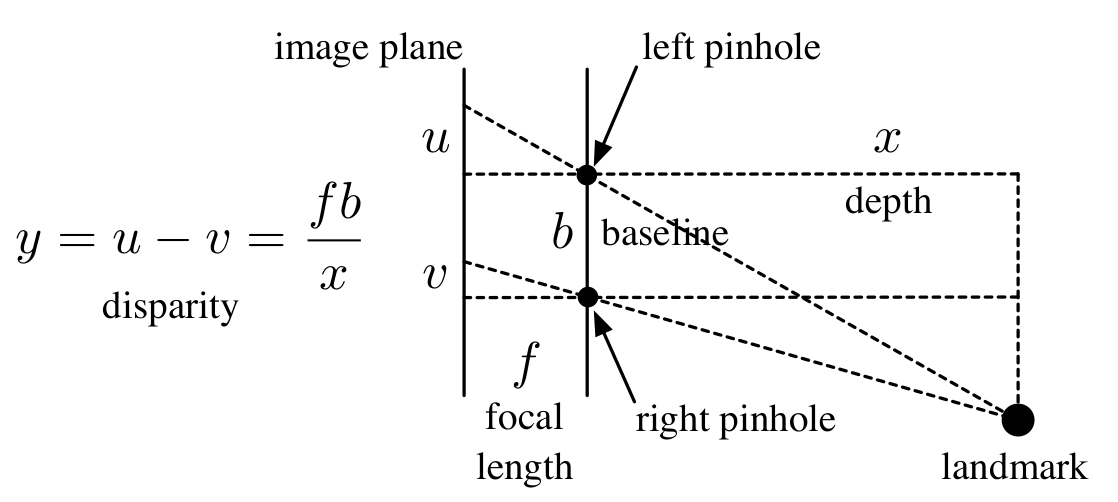
\includegraphics[width=0.6\textwidth]{figures/barfoot_stereo.png}
    \caption{Stereo depth estimation toy model \cite{barfoot2017state}}
    \label{fig:barfoot_stereo}
 \end{figure}
%
where $y=u - v$ is a disparity measurement ($u$ and $v$ are pixels corresponding to the projection of the landmark in each camera), $f$ is the focal
length of the cameras (in pixels), $b$ is the horizontal distance between cameras (the baseline, in meters), a $n_y \approx \Gaussian{0}{\sigma_y^2}$ 
is the measurements noise (in pixels), assumed to be Gaussian. We also assume that we have prior knowledge about the 
estimated value $x_p$, with a standard deviation of $\sigma_p$.

To ground the problem, we will assign sensible values to the problem (same as \cite{barfoot2017state}):
%
\begin{gather*}
    x_{true} = 22~[m], \quad x_p = 20~[m], \quad \sigma_p = 3~[m] \\
    f = 400~[pixels], \quad b = 0.1~[m], \quad \sigma_y = 0.3~[pixels]   
\end{gather*}
%
where $x_{true}$ is the true depth that we seek to estimate.

Notice that the prior standard deviation is quite big, assuming a great uncertainty about the prior value. We simulate noisy measurements by drawing samples 
$\{y_{i \in [1..m]}\}$ of the measurement model using $x_{true}$ (we drew $m=10$ measurements). For a low dimensional problem such as this one, 
it is possible to compute the full posterior distribution $p(x|\bfy)$ by numerical integration, which is referred to as the "grid approximation" by 
\cite{mcelreath2018statistical}. We can make this computation almost arbitrarily precise since the computations are quite cheap. The prior and density distribution are represented in \figRef{fig:MAP_stereo1D}. Applying the Laplacian approximation to
compute a posterior approximation involves minimizing the negative log-likelihood:

\begin{equation}
    \frac{1}{2 \sigma_p^2}(x - x_p)^2 + \frac{1}{2\sigma_y^2} \sum_{i=1}^m (\frac{fb}{x} - y_i)
\end{equation}

Finding the MAP and approximating the covariance deviation of $x$, we can plot the MAP posterior along with its numerical computation in \figRef{fig:MAP_stereo1D}. 
Both computations result in largely overlapping functions: the main mass of the real posterior density function is captured by the Laplacian approximation.
However, notice that the real posterior distribution is not symmetrical contrary to the prior it derives from. This means that, contrary to its Gaussian approximation, the mean of the
of the real posterior is not equal to its mode. 

\begin{figure}[h]
    \centering
    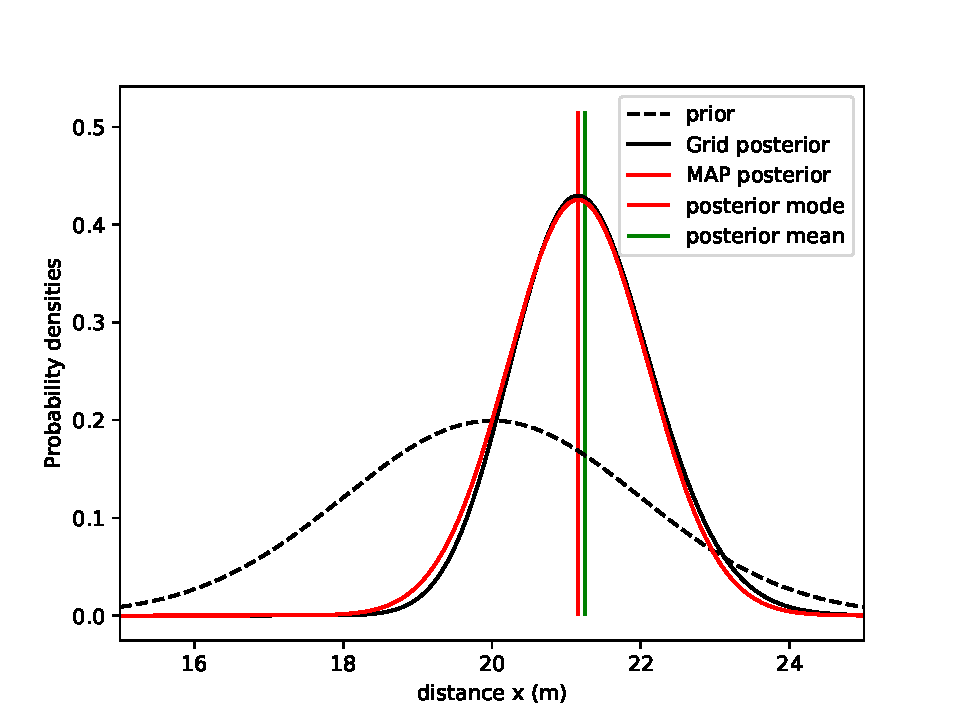
\includegraphics[width=0.8\textwidth]{figures/MAP_stereo1D.pdf}
    \caption{Representation of posterior inference on the toy problem. Dotted black: prior on $x$, 
    continuous black: numerical "grid" integration of the posterior, continuous red: Laplacian approximation of the posterior. 
    Vertical lines: red=MAP, green=mean of the posterior. The true value (22 m) is reasonably close to the MAP given the variance 
    of the posterior distribution.
    }
    \label{fig:MAP_stereo1D}
 \end{figure}




\section{Lie groups for state estimation}
Some of the state variables that we manipulate in robotics are challenging since they do not belong to vector spaces. Some of the equations
involved in the Gauss-Newton algorithm cannot be directly applied without extra care when it is the case.
These variables live on smooth manifolds, also known as Riemannian manifolds. 
Many examples of Riemannian geometry arise in data science and robotics \cite{miolane2020geomstats}. 
Besides, many of these robotics state variables also exhibit a group structure which, together with the smooth manifold
property, define the so-called Lie group.
In this section, we will provide the minimal concepts regarding smooth manifolds and Lie groups that are useful to the roboticist. In particular, we will show 
that a limited number of notation changes can be made to the Gauss-Newton algorithm to accommodate for the special structure of these variables.



\subsection{Smooth manifold structure}
A \textit{smooth manifold} $\cM$, or differentiable manifold, is a topological space that can be pictured as a smooth surface embedded in a higher dimensional vector space.
The smoothness property means that to each surface point $\bfx$ corresponds a unique tangent \mbox{(hyper-)plane} $\cT_{\bfx}\cM$, called the tangent space 
(there are no spikes or edges on the surface). The tangent space is a vector space on which traditional calculus operations are applicable. The dimension of this 
vector space is equal to the dimension of the surface as well as the degrees of freedom of its elements.
We will denote by $p$ the dimension of the space in which the manifold is embedded and by $n$ the dimension of the manifold.
Note that by definition $n \leq p$.  
An element of tangent space at $\bfx$, $\bftau\hhat \in \cT_{\bfx}\cM$ can naturally be decomposed as a linear combination 
of the tangent space basis vectors $E_i$. We can therefore define an element by its coefficient, which is the vector $\bftau \in \Reals^n$, called the cartesian tangent vector.
The \textit{hat} and \textit{vee} are mutually inverse linear maps permit to pass back and forth from $\cT_{\bfx}\cM$ to $\Reals^m$, which are therefore isomorphic:
%
\begin{align}
    \text{Hat} ~ :& \quad\quad \Reals^n \rightarrow \cT_{\bfx}\cM; \quad\quad \bftau \rightarrow \bftau\hhat = \sum_{i=1}^n\tau_i E_i  \\
    \text{Vee} ~ :& \quad\quad \cT_{\bfx}\cM \rightarrow \Reals^n; \quad\quad \bftau\hhat \rightarrow (\bftau\hhat)\vvee = \bftau = \sum_{i=1}^n\tau_i \bfe_i
\end{align}
%
where $\bfe_i$ are basis vectors of $\Reals^n$.

Vector spaces operations such as the addition of a vector to a point or subtraction of two vectors do not apply in Riemannian geometry. For instance, if we
take a point on a sphere (the 2-sphere embedded in the 3-dimensional Euclidean space for instance) and add to it an arbitrary vector, we do not get in general
another point on the sphere. These operations have equivalent in the \textit{retraction} and its inverse.
Retraction pulls an element from the local tangent space back to the manifold as represented in \figRef{fig:manifold}. We denote retraction and its inverse as 
$\oplus$ and $\ominus$:
%
\begin{align}
            \text{Retraction}~:&\quad\quad \bfx_2 = \bfx_1 \oplus \bftau   \\
    \text{Retraction inverse}~:&\quad\quad \bftau = \bfx_2 \ominus \bfx_1  \\
\end{align}

% Note that we informally define the retraction operator and its inverse as operations dealing with the 

\begin{figure}[h]
    \centering
    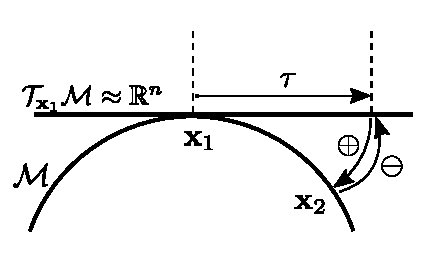
\includegraphics[width=0.5\textwidth]{figures/manifold.pdf}
    \caption{Manifold, tangent space, retraction and inverse retraction operations}
    \label{fig:manifold}
\end{figure}

When dealing with a collection of elements $\bfx^i$ living in their respective manifold $\cM^i$, it is often convenient to define a composite manifold
as the concatenation $\cM_c \triangleq \left<\cM^1, \dots, \cM^M \right>$. The element of this composite manifold is denoted by $\cX$.
We will also write composite equivalent of the retraction operation $\oplus$ and 
its inverse $\ominus$. It consists in applying operatrions to individual elements of the manifold and its tangent space:

\begin{equation}
    \cX=
    \begin{bmatrix}
        \bfx^1 \\
        \vdots \\
        \bfx^M
    \end{bmatrix},
    \quad
    \cX \oplus \bftau
    =
    \begin{bmatrix}
        \bfx^1 \oplus \bftau^1 \\
        \vdots \\
        \bfx^M \oplus \bftau^M
    \end{bmatrix}
    \quad
    \cX_2 \ominus \cX_1
    =
    \begin{bmatrix}
        \bfx^1_2 \ominus \bfx^1_1 \\
        \vdots \\
        \bfx^M_2 \ominus \bfx^M_1
    \end{bmatrix}
\end{equation}



\subsection{Back to the MAP optimization problem}
\label{sec:manifold_GN}
Elements of the tangent space can be interpreted as steps that we can make to go from one point of the manifold to another.
This ties closely to the notion of Gaussian steps that we defined earlier. We will now consider that the estimated state $\cX$
is an element of a composite manifold. In this case, the Gaussian steps of \eqRef{eq:gaussian_step}
are in the composite manifold tangent space and the step updates write:

\begin{equation}
    \check{\cX} := \check{\cX} \oplus \Delta \bfx^*
\end{equation}
%
obtained by solving
%
\begin{equation}
    \Delta \bfx^* = \argmin_{\Delta \bfx} ||\bfr(\check{\cX} \oplus \Delta \bfx)||^2.
\end{equation}


Concerning residual formulation in \eqRef{eq:error_expectation}, if the measurement $\bfz_i$ is itself an element of a manifold, then the cartesian minus needs to be replaced:

\begin{equation}
    \bfe_i(\cX_{S_i}) = \bfh(\cX_{S_i}) \ominus \bfz_i,
\end{equation}

Note that many state variables actually belong to vector spaces (such as the robot position), which are trivial manifolds. For those, the $\oplus$ and $\ominus$ operators
simply reduce to the addition and subtraction of cartesian vectors.  



\subsection{Uncertainty in manifolds, jacobians}
Our state variables are random variables approximated by multivariate Gaussian distribution, that can be summarized by their mean vector and covariance matrix.
These concepts need to be slightly modified to account for the manifold nature of some of these. We will see how to define Gaussian distribution on manifolds.
Let us $\bftau \in \Reals^n$ be a small perturbation around a point $\bar{\bfx} \in \cM$, so that we can write:
%
\begin{equation}
    \bfx = \bar{\bfx} \oplus \bftau, \quad \bftau = \bfx \ominus \bar{\bfx}
\end{equation}
%
where $\bar{\bfx}$ designate the mean value of the distribution on $\bfx$. 
We define a zero mean "cartesian" Gaussian distribution on the tangent space, the covariance being defined as:

\begin{equation}
    \Cov_{\bfx} = \mathbb{E}[\bftau\bftau^{\top}] = \mathbb{E}[(\bfx \ominus \bar{\bfx})(\bfx \ominus \bar{\bfx})^{\top}] \in \Reals^{n \times n}
\end{equation}
%
where $\mathbb{E}[\cdot]$ denotes the expectation operator.
By a slight abuse of notation, we note that the manifold distribution is $\bfx \approx \Gaussian{\bfx}{\Cov_{\bfx}}$

As an illustration, the group of unit quaternions $\mathbb{H} = \left\{ \bfq \in \Reals^4~|~\bfq \odot \bfq^*=1 \right\}$ under quaternion multiplication 
$\odot$ is a manifold (the $S^3$ sphere, p=4 and n=3) \cite{sola2012quaternion}. 
The tangent space is the set of antisymmetric matrices, which is isomorphic to the angle axis rotation vectors $\bftheta \in \Reals^3$.
If we naively define the covariance matrix of a quaternion as \mbox{$\mathbb{E}[(\bfq - \bar{\bfq})(\bfq - \bar{\bfq})^{\top}] \in \Reals^{4 \times 4}$}, 
this covariance matrix is ill-defined. The covariance is instead defined as a $3 \times 3$ real matrix on the angle axis space.

In general, covariances can be propagated through nonlinear function of random variables using the chain rule. For instance, if $\bfx \in \Reals^{n_x}$ and 
$\bfy \in \Reals^{n_y}$ are cartesian multivariate Gaussian distribution related by the nonlinear function $f$, propagating the $\bfx$ covariance 
$\Cov_{\bfx} \in \Reals^{n_x \times n_x}$ through f writes:

\begin{equation}
    f~: \bfx \in \Reals^{n_x} \rightarrow \bfy \in \Reals^{n_y}, \quad \quad \Cov_{\bfy} \approx 
                \left.\frac{D f}{D \bfx} \right|_{\bfx}   \Cov_{\bfx}    \left.\frac{D \bfy}{D \bfx}\right|_{\bfx}^{\top}
    \label{eq:cov_propagation}
\end{equation}

The same equation applies for random variables $\bfx \in \cM_{\bfx}$ and $\bfy \in \cM_{\bfy}$ living on manifolds. The definition of jacobians has however
to be redefined as:

\begin{equation}
    \frac{D f}{D \bfx} \triangleq \lim_{\bftau \to 0} \frac{f(\bfx \oplus \bftau) \ominus f(\bfx)}{\bftau}
\end{equation}

These jacobians also play a central role in the derivation of the residual jacobians \eqRef{eq:res_jacobian}.
Examples of manifold jacobian derivations in the context of Lie groups can be found in \cite{sola2018micro}.  



\subsection{Lie groups for robotic state estimation}
A \textit{group} ($\cG$, $\circ$) is a couple comprised of a set $\cG$ and a composition law $\circ$ that satisfy the group axioms:

\begin{align}
    \text{Closure under}~\circ~:&~\bfx \circ \bfy \\ 
    \text{Associativity}~\circ~:&~(\bfx \circ \bfy) \circ \bfz = \bfx \circ (\bfy \circ \bfz) \\ 
    \text{Identity element}~\cE~:&~\bfx \circ \cE = \cE \circ \bfx = \bfx \\ 
    \text{Inverse existence}~\bfx^{-1}~:&~\bfx^{-1} \circ \bfx = \bfx \circ \bfx^{-1} = \cE
\end{align}
$\forall~\bfx,\bfy,\bfz \in \cG$.

Simply stated, a \text{Lie group} is a group whose elements live in a smooth manifold $\cM$.
A vector can represent a displacement from one point to another along a straight line in the euclidean space, or directly a point (displacement from the origin).
Analogously, an element of a Lie group represents a path from one element to another along a geodesic of the manifold, or directly an element of the group 
(displacement from the identity element $\cE$).

In particular, the identity element $\cE$ relates to a notion of a global reference from which each element of the manifold can be compared.
The tangent space at this element is called the Lie algebra $\mathfrak{m} \triangleq \cT_{\cE}\cM$.

Let us compute the retraction operations in the case of Lie groups. We will follow the example of 3D rotations as they are of great use in robotics and provide
good intuitions regarding the general behavior of Lie groups.
The group of 3D rotations is defined as the Special Orthogonal group in 3D: 
%
\begin{equation}
    \SO(3) = \left\{\Rot{}{} \in \text{GL}(n,\Reals) | \Rot{}{}\Rot{}{}^{\top}=\Rot{}{}^{\top}\Rot{}{}=I,~det(R)=1\right\}
\end{equation}
%
under matrix multiplication.


Firstly, properties that make $SO(3)$ a group are immediate from the properties of matrix multiplication:
%
\begin{itemize}
    \item Closure under the matrix product
    \item Associativity through the matrix product
    \item Identity element $\bfI_3$
    \item Inverse element $\Rot{}{}^{-1} = \Rot{}{}^{\top}$ (from the group definition)
\end{itemize}

Let us explicit the manifold structure of $\SO(3)$. First, the topology of its corresponding manifold is the $S^3$ sphere.
It can be shown \cite{sola2018micro} that taking the time difference of a rotation matrices results in an element of its local tangent space:

\begin{equation}
    \dot{\Rot{}{}} = \Rot{}{} [\angvel{}{}]_{\times} \in \cT_{\Rot{}{}}\SO(3)    
\end{equation}
%
where $[\cdot]_{\times}$ is the skew-symmetric operator associated to the cross product. 
\mbox{$[\angvel{}{}]_{\times} = \angvel{}{} \times \cdot$}. The Lie algebra $\so(3)$ is therefore the 3 dimensional vector space of antisymmetric matrices.
For a constant $\angvel{}{}$, this defines an ordinary differential equation (ODE) whose solution
is $\Rot{}{}(t)=\Rot{}{0}\exp([\angvel{}{}]_{\times}t)$ where exp is the matrix exponential:

\begin{equation}
    \exp(\bfA) = \sum_{k=0}^{\infty} \frac{\bfA^k}{k!}.
\end{equation}

For $\SO(3)$ and most other Lie groups, properties of the Lie algebra simplify the infinite sum of the matrix exponential to a simpler closed-form formula. 
In the $\SO(3)$ case, this formula is known as the Rodriguez equation:

\begin{equation}
    \Exp(\bftheta) = \exp([\bftheta]_{\times}) = \bfI + [\bfu]_{\times}\sin(\theta) + [\bfu]_{\times}^2(1 - \cos(\theta))
\end{equation}
%
where $\bftheta \triangleq \theta \bfu \in \Reals^3$ and $\theta$ is the norm of the rotation vector (angle in radiant) and $\bfu$ its unitary direction.
Finally, we have denoted by $\Exp$ the composition of the $hat$ operator ($\bftheta\hhat \triangleq [\bftheta]_{\times} \in \so(3)$). 
The inverse operation that maps elements from the group to the Lie algebra is defined as the $\Log$ map. A general representation of
Lie group operation can be found in \figRef{fig:lie_group}

We all of that in mind, the link with the Riemannian manifold terminology becomes clearer. We can compose a rotation with
an increment $\prescript{1}{}{\bftheta}$ taken in the tangent space at $\bfx_1$ to obtain another rotation: $\Rot{}{2} = \Rot{}{1}\Exp(\prescript{1}{}{\bftheta})$.
This corresponds to the $\oplus$ retraction operator. Conversely, the inverse of the retraction $\ominus$ corresponds to the application of The
logarithm on the relative rotation as described here:

\begin{align}
    \Rot{}{2} &= \Rot{}{1}\oplus \prescript{1}{}{\bftheta} = \Rot{}{1} \Exp(\prescript{1}{}{\bftheta})  \\ 
    \prescript{1}{}{\bftheta} &= \Rot{}{2}\ominus \Rot{}{2} = \Log(\Rot{}{1}^{\top}\Rot{}{2}) 
\end{align}

\begin{figure}[h]
    \centering
    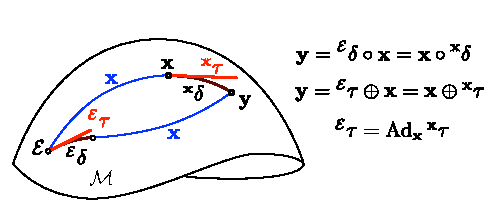
\includegraphics[width=0.7\textwidth]{figures/lie_group.pdf}
    \caption{Representations of a Lie group including the identity element $\cE$, operations of composition
    between increments and relations between a tangent space increment at the identity $\prescript{\cE}{}{\bftau}$ 
    and at the local element $\prescript{\bfx}{}{\bftau}$ through the adjoint matrix $\text{Ad}_{\bfx}$. Figure adapted from \cite{sola2018micro}.}
    \label{fig:lie_group} 
\end{figure}

\begin{figure}[h]
    \centering    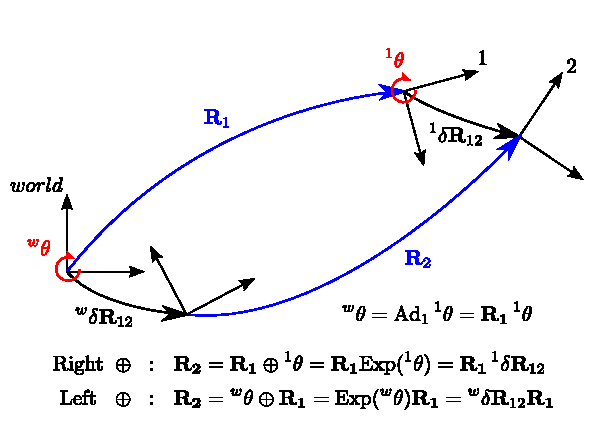
\includegraphics[width=0.7\textwidth]{figures/rotation_exp_log.pdf}
    \caption{Representation of $\SO(3)$ Lie groups operations. Note that we represented frames with different origins
    for better readability while the group elements only represent pure rotations (no translation). $world$ is the "global" reference 
    frame of the problem to which we assign the identity element of $\SO(3)$: $\bfI_3$. $1$ and $2$ are two frames of reference
    defined by their orientations \wrt $world$, $\Rot{}{1}$ and $\Rot{}{2}$. $\delta \Rot{}{12}$ is the relative rotation
    between elements $\Rot{}{1}$ and $\Rot{}{2}$ and can be computed using the exponential map on the angle axis $\bftheta$ expressed
    in $world$ or local frame, depending on whether we use the right or left $\oplus$ operator.}
    \label{fig:rotation_exp_log} 
\end{figure}

In robotics terms, $\prescript{1}{}{\bftheta}$ is the axis angle representation of the relative rotation $\prescript{1}{}{\delta \bfR}_{12} = \Rot{}{1}^{\top}\Rot{}{2}$ and
\textit{local} rotations represent the orientation of reference frames in a \textit{global} world reference frame. The identity element, therefore, corresponds 
to the world frame. For Lie groups, an additional $\oplus$ operator exists that retracts and composes vectors at the Lie algebra instead of
the local tangent space, the left-$\oplus$. The local operator, that corresponds to the manifold retraction, is called the right-$\oplus$. 
The Adjoint $\text{Ad}_{\bfx}\cM$ is an operatormaps elements from the local tangent space to the Lie algebra. 

\begin{equation}
    \prescript{\cE}{}{\bftau} = \text{Ad}_{\bfx}\cM \prescript{\bfx}{}{\bftau} 
\end{equation}

For rotation matrices, the adjoint matrix is $\text{Ad}_{\bfR}\SO(3)=\bfR$: to change the reference frame of the angle axis from local to global reference, it needs
to be rotated from one frame to another. Those operations are illustrated in \figRef{fig:rotation_exp_log}.


%
%
%
\section{Factor graphs: a visual language for robotics estimation}
\label{sec:factor_graphs}

A crucial aspect of solving the MAP problem is the factorizibility of the likelihood function. This represents the fact that the problem
exhibits a particular structure that has important computational implications. We will first explain how this factorization can be described 
visually using a graphical model known as the \textit{Factor Graph} and then link this representation to the sparsity of the matrices involved
in solving the NLLS problem.


\subsection{Factor Graph representation}
Let us consider the toy example represented in \figRef{fig:toy_problem}. 
We wish to estimate the trajectory of a differential robot, that is its states at chosen timestamps called \textit{\keyframes}, and remarkable elements 
of the environment, called \textit{landmarks}. We suppose that this robot is equipped with an odometer, whose measurements integrated over time provide relative 
transformations between \keyframes, and an exteroceptive sensor that provides relative measurements between \keyframes~and landmarks.

\begin{figure}[h]
    \centering
    \begin{subfigure}{.49\linewidth}
        \centering
        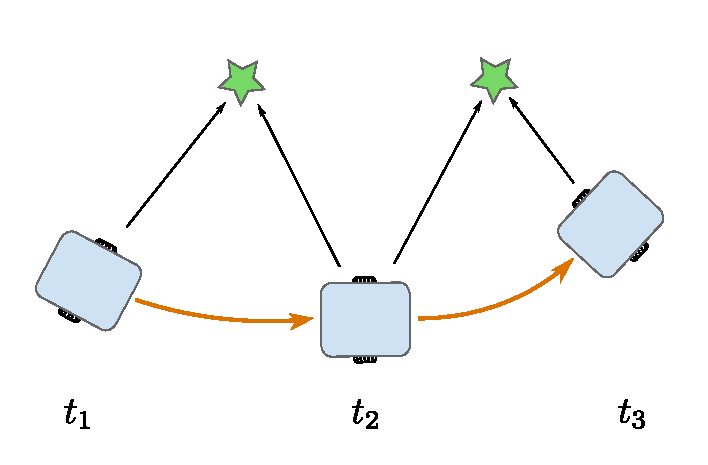
\includegraphics[width=\textwidth]{figures/toy_example.pdf}
        \caption{\label{fig:toy_problem}}
    \end{subfigure}%
    \hfill
    \begin{subfigure}{.49\linewidth}
        \centering
        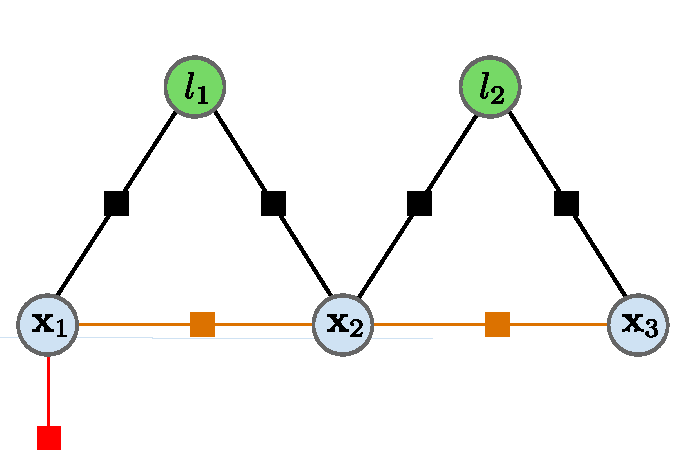
\includegraphics[width=\textwidth]{figures/toy_factor.pdf}
        \caption{\label{fig:toy_factor}}
    \end{subfigure}%
    \caption{(\subref{fig:toy_problem}): toy estimation problem, a differential drive robot equipped with an odometer moves in 
    an scene with landmarks represented by stars. (\subref{fig:toy_factor}): factor graph representation the problem, the estimated variables are represented by circles 
    (blue for robot \keyframes, green for landmarks) and factors by squares (orange for odometry, black for exteroceptive sensor, red for the prior).}
\end{figure}

In this case, the state variables are $\cX = \{ \bfx_1, \bfx_2, \bfx_3, l_1, l_2\}$  and measurements $\cZ = \{ z_{o,1}, z_{o,2}, z_{e,1}, z_{e,2}\}$.
We also apply a prior on the pose of the first \keyframe of the trajectory, which can be understood as fixing the frame origin of the reference 
frame in which the estimation is done.

The factorization of the likelihood of \eqRef{eq:likelihood_factorization} in this example writes:
%
\begin{align}
    p(\cX | \cZ) \propto 
    ~&{\color{Red} \phi_0({\color{Blue} \bfx_{0}})} \\ 
    ~&{\color{Orange} \phi_1({\color{Blue} \bfx_1}, {\color{Blue} \bfx_2}) \phi_2({\color{Blue} \bfx_2}, {\color{Blue} \bfx_3})} \\ 
    ~&{\color{Black} \phi_3({\color{Blue} \bfx_1}, {\color{Green} l_1}) \phi_4({\color{Blue} \bfx_2}, {\color{Green} l_1}, {\color{Green} l_2}) \phi_5({\color{Blue} \bfx_3}, {\color{Green} l_2})} \\ 
\end{align}

This factorization can be represented as a \textit{factor graph} as seen in \figRef{fig:toy_factor}. 
factor graphs are popular graphical models \cite{koller2009probabilistic} that can describe a vast family of statistical models \cite{loeliger2004introduction}.
A factor graph in the most general sense is a bipartite graph that represents the factorization of a function of several variables. 
We adopt the visual notation commonly found in robotics: round nodes for variables, square nodes for factors, edges represent the dependency 
of each factor on a subset of variables. Dellaert and Kaess \cite{dellaert2006square} were the first to
recognize the link between NLLS problems and factor graphs \cite{dong2019minisam}. Over the last two decades, they have grown in popularity among roboticists as a visual language to describe 
estimation problems \cite{dellaert2017factor} and planning problems \cite{dong2016motion}. As Frank Dellaert puts it \footnote{Citation from a recent talk,
see \href{https://www.youtube.com/watch?v=-yCC7mpgL4w}{this video}, around 15:30.}, factor graphs are "an amazing thing to write on blackboards".% and white boards". 
Aside from providing insights over the computational structure of the problems, they can be used as a common language between engineering teams
to convey insights about the nature of the problems to solve.

% The SLAM problem hereby represented as a factor graph in only one example of the vast family of estimation problem that can be modeled as a factor graph
% (other including \eg target tracking, structure-from-motion, control and planning \cite{}). 

Many specialized solvers \cite{grisetti2011g2o, kaess2012isam2, ila2017slam++} have been implemented that exploit the sparse structure of these 
problems. A discussion of the particularities of factor graph-based NNLS solvers can be found in \cite{dellaert2017factor, sola2017course}.




\subsection{Sparsity of the NLLS problem}

The jacobian matrix of the residuals $\bfJ \in \Reals^{M \times N}$ is a big sparse matrix of dimensions 
\begin{itemize}
    \item M rows = $\sum_{i=1}^{m}dim(\bfe_i) \rightarrow~$ the sum of residual dimensions
    \item N columns = $\sum_{i=1}^{n}dim(\cT_{\bfx_i}\cM_i)~\rightarrow$ the sum of variables tangent spaces dimensions 
\end{itemize}   

Each block column corresponds to one of the state variables and each row corresponds to a residual. For each row, only the blocks corresponding to the
state variables that the residual depends on are non-zero. For instance, the matrix corresponding to the toy problem described in \figRef{fig:toy_problem} is:
\begin{equation}
    \bfJ=
    \begin{pmatrix}
        J^{p}_{\bfx_1} &   &     &     &     \\
       J^{o_1}_{\bfx_1} & J^{o_1}_{\bfx_2}  &     &     &     \\
                       & J^{o_2}_{\bfx_2}  & J^{o_2}_{\bfx_3}   &     &     \\
       J^{e_1}_{\bfx_1} &                  &     &  J^{o_2}_{\bfl_1}   &     \\
                       & J^{e_1}_{\bfx_2}  &     &  J^{e_1}_{\bfl_1}   &     \\
                       & J^{e_2}_{\bfx_2}  &     &     &  J^{e_2}_{\bfl_2}   \\
                       &                  & J^{e_3}_{\bfx_3}    &     &  J^{e_3}_{\bfl_2}   \\
    \end{pmatrix}
    \label{eq:sparse_jac}
\end{equation}



The approximate Hessian matrix $\bfH \in \Reals^{N \times N}$ displays a similarly remarkable sparsity that makes the resolution of the linear system
at each step very efficient. Algorithms such as the Schur complement, Cholesky factorization, and QR factorization were applied by different authors to the 
problem of SLAM and estimation. Descriptions of these factorizations can be found in \cite{sola2017course, dellaert2017factor}.







% CONCLU
%\chapter{Object-level vision}
\label{chp:object_level}
\minitoc

The field of computer vision comprises a wide range of methods to extract information about the real world from images taken by digital cameras. This information can be used to infer the structure of the environment (mapping or object tracking), about the movement of the system to which is attached the camera (localization), or both at the same time (Simultaneous Localization And Mapping, \aka\ SLAM). In the context of robotics, the images are obtained one after an other at a constant rate. This leads to a somewhat continuous evolution of the image appearance, which can be leveraged by in various ways  (feature tracking, motion models etc.). We are here interested in solving SLAM, which is the most general application of this methods and is used when a robot needs to localize itself in an a priori unknown environment. A vast literature of dedicated algorithms have been developed in this regard, with approaches ranging from geometrical constraints using sparse feature detection (CITE ORBSLAM and 2 others) or photometric consistencies [DTAM, LSD, DSO], certain methods combining ideas from both approaches [SVO2].

These algorithms aim at being generalizable to any kind of environments and have their respective strengths and weaknesses [CITE Review]. Although open-source code is available for most, these pieces of software may be difficult to integrate in other frameworks. Besides, though providing quite accurate localization, maps obtained from these methods are rarely immediately useful, lacking semantic information about the scene usable by a legged robot. 

In this thesis, rather than investing time and energies in new vision processing algorithms, we chose to focus our attention on legged-robot state estimation. In particular, we are interested in localizing the robot with respect to objects of interest such as stairs, tables or the like, whose geometrical models are known.
Approaches based on object-level measurement can provide an affordable alternative, and are readily available. These systems assume the presence of known objects in the scene which can be detected in the images. Dedicated algorithms can then infer the object pose relative to the camera, which can be used to build \textit{object-level SLAM} systems. 

In this chapter, we present two measurements models based on available software, that permit to implement this paradigm. The first one 
uses unique \apriltag\ fiducial markers \cite{wang2016iros} that are disposed sparsely in the scene. The second uses a deep learning-based method \cite{labbe2020cosypose}
to obtain relative poses from object of interest, such as stairs. Instead of artificially augmenting the environment with fiducial markers, we assume that objects of interest exist in the scene, whose CAD models are known. 
Both systems lack ways to estimate the uncertainty of their output and we therefore propose methods for the computation of the measurements covariances.

In both models, we assume that we have a calibrated camera, and that the images have been corrected for distortions. The camera reference frame $C$ has its origin at 
the camera optical center and follows the convention X-Y-Z = Righ-Down-Front, Front being the optical axis direction, looking through the lens. This chapter starts by introducing the measurement model based on a general 6D factor used by both systems. Methods to recover the covariance of both algorithms are then given. For applications fusing these models with IMU data, please refer to \ref{chp:absolute_vi}
and \ref{chp:cosyslam}.



\section{Relative 6D pose factor}
Let's assume that an algorithm provides us $\Tm{C}{O} \in \SE(3)$, a measurement of the pose of an element 
of the scene with an attached frame $O$ with respect to the camera frame $C$.
The kinematic chain of the problem described in \figRef{fig:camera_object_chain} unrolls as 
$\T{W}{O} = \T{W}{B}\T{B}{C}\T{C}{O}$ where W and B correspond to the world and body frames. $\T{B}{C}$ corresponds to the extrinsic pose 
of the camera that has to be calibrated.
Given measurement $\Tm{C}{O}$, this relation can therefore be turned into a residual relating 
the robot pose, the camera extrinsics, and the object pose:

\begin{align}
    \bfe_V (\T{W}{B}, \T{B}{C}, \T{W}{O}) 
    &= \left[ (\T{W}{B}\T{B}{C})^{-1}\T{W}{O} \right] \ominus \Tm{C}{O} ~ \in \Reals^6 \\
    &= \Log_{\SE(3)} ( (\T{W}{B} \T{B}{C} \Tm{C}{O})^{-1} \T{W}{O}) ~ \in \Reals^6
\end{align}
%
where here $\Log_{\SE(3)}$ denotes the log map on $\SE(3)$.

We also assume that we have access to the covariance of this measurement 
\mbox{$\Cov_V \in \Reals^{6 \times 6}$}. 

This factor is general enough to be used in two applications that we successively describe, based on \apriltag\ fiducial markers and CosyPose. For both, we explain the
algorithm behind the pose measurements and propose covariances models

% We will now describe two applications of this factor, one using \apriltag\ fiducial markers and one using 
% a deep-learning object pose estimation algorithm.

\begin{figure}
    \centering
    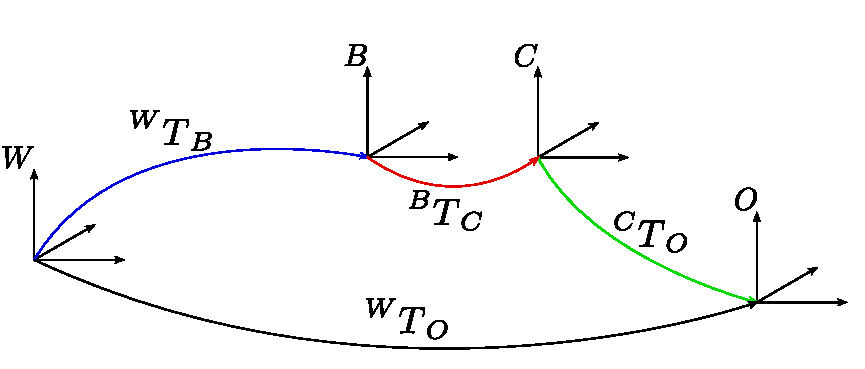
\includegraphics[width=0.7\textwidth]{figures/kin_tree_object.pdf}
    \caption{Kinematic tree of the object/camera measurement model}
    \label{fig:camera_object_chain}
\end{figure}


%
%
\section{Fiducial marker}
\subsection{Markers Pose estimation algorithms}

Fiducial markers (such as ARToolkit \cite{kato1999marker}, ARTag \cite{fiala2005artag}, ArUco \cite{garrido2014automatic}) are widely used in robotics and Augmented Reality (AR) applications as they provide an easy way to obtain a relative 6D pose 
between a calibrated camera and the marker. These markers are designed so that they are uniquely and robustly identifiable in any scene 
\cite{wang2016iros,romero2018speeded}. For square markers, the outputs of the algorithm are sub-pixel projections of the square corners, whose 
corresponding position in the local reference frame of the tag is known (using the tag dimensions). Recovering their pose is then an instance 
of the Perspective n Point (PnP) algorithm, which requires at least three 2D-3D correspondences to compute the 3D pose. 
A vast literature has been written on the topic, many methods relying on efficient analytical models
\cite{gao2003complete, lepetit2009epnp, collins2014infinitesimal, terzakis2020consistently}, sometimes refined by a nonlinear maximum likelihood step. 

A known problem of fiducial markers is the orientation ambiguity for noisy images. Close to fronto-parallel pose (identical orientation as 
the camera frame), the estimated orientation can jump between two solutions of orientations several tenths of degrees apart 
\cite{collins2014infinitesimal}. 
This problem has been addressed by an analytical algorithm called Infinitesimal Plane-based Pose Estimation \cite{collins2014infinitesimal} that can 
provide both ambiguous solutions so that the end-user may make an informed choice based on other data.

\subsection{Covariance model}
Obtaining a covariance of the estimated transformation is an important step toward the integration of these measurements in a sensor fusion algorithm.
For methods relying on a maximum likelihood nonlinear optimization refinement step, one might invert the Hessian matrix at the optimum to obtain a covariance 
(as explained in \secRef{sec:map_covariance}).
Eq. (23) in \cite{urban2016mlpnp} shows an analytical formula to compute pose uncertainty from pixel noise.
The presented method in this paper uses a careful parameterization of the homogeneous coordinates associated with 2D features to develop
a maximum likelihood PnP algorithm.  However, the formulation is particular to the choice of parameterization described in the paper and, 
therefore, we think that a simpler yet equivalent formulation is possible. This model is proposed in our work \cite{fourmy2019absolute}. 

Usually, when a nonlinear mapping of noise variables from one space to another is available, we can propagate the covariance through the nonlinearity
as shown in Eq. \eqRef{eq:cov_propagation}.  
Instead of directly obtaining Jacobians from the PnP algorithms, we found that a natural way to proceed is to take the opposite 
direction as follows. It should somehow be possible, knowing the marker size and the relative pose measurement, and assuming pixel noise, to
recover $\Cov_{\T{}{}}$. A simple model of pixel noise is to assume isotropic Gaussian noise on the pixels. If we stack four pixel (the four tag corners) 
$\bfx_i = [u_i, v_i] \in \Reals^2$ in the column vector $\bfx = [\bfx_1~\bfx_2~\bfx_3~\bfx_4]^{\top}$, we have therefore that
$\bfx$ is corrupted by a Gaussian noise $\Cov_{\bfx} = \sigma_{x}^2 \bfI_8$, where $\sigma_{x}$ usually takes values of 1 or 2 pixels.
The PnP algorithm provides us with a function $\text{pnp}$ defined as:

\begin{equation}
    \begin{split}
        \text{pnp}_w: \Reals^8 &\rightarrow \SE(3) \\
                           \bfx &\rightarrow \T{C}{O} = \text{pnp}_w(\bfx)
    \end{split}
\end{equation}
%
where w denotes the dependency on the width of the marker. This $\text{pnp}_w$ function implementation depends on the specificities of the PnP algorithm used and  
is in general hard to analytically differentiate. Instead, if we consider the inverse function

\begin{equation}
    \begin{split}
        \text{proj}_w: \SE(3) &\rightarrow \Reals^8 \\
                           \T{C}{O} &\rightarrow \bfx = \text{proj}_w(\T{C}{O})
    \end{split},
\end{equation}
%
that maps the relative pose to the projection of the tag in the image, a rather simple jacobian expression can be derived using the chain rule, as follows.

Let's define the marker corner coordinates in the marker frame like shown in \figRef{fig:tag_coordinate_frame}. As a convention 
\cite{wang2016iros} we order the corners counter-clockwise starting from bottom left (looking straight at the tag). 

\begin{equation}
    c =
    \begin{pmatrix}
    c_1 \\ c_2 \\ c_3 \\ c_4
    \end{pmatrix}
    ~~
    c_1 =  \begin{pmatrix} -\frac{w}{2} \\ \frac{w}{2} \\ 0 \end{pmatrix}
    ~ 
    c_2 =  \begin{pmatrix} \frac{w}{2} \\ \frac{w}{2} \\ 0 \end{pmatrix}
    ~
    c_3 =  \begin{pmatrix} \frac{w}{2} \\ -\frac{w}{2} \\ 0 \end{pmatrix}
    ~
    c_4 =  \begin{pmatrix} -\frac{w}{2} \\ -\frac{w}{2} \\ 0 \end{pmatrix}.
\end{equation}

%
\begin{figure}
    \centering
    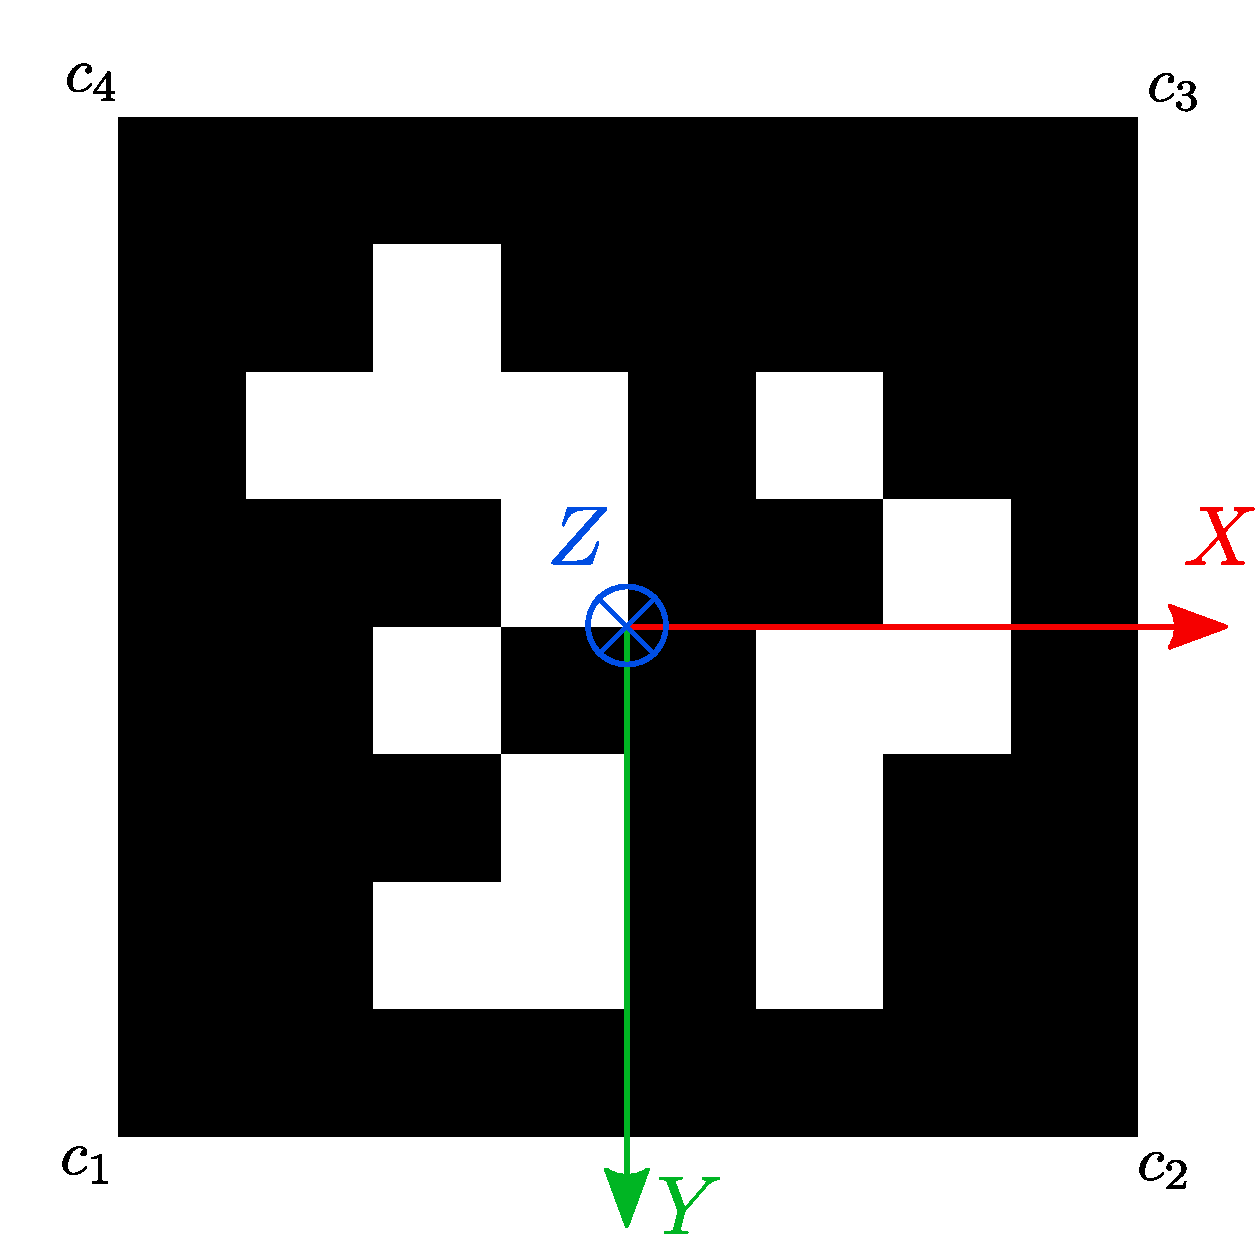
\includegraphics[width=0.5\textwidth]{figures/tag12_frame.pdf}
    \caption{\apriltag~local coordinate systems and corners conventions \cite{wang2016iros}}
    \label{fig:tag_coordinate_frame}
\end{figure}

Then, assuming that images are corrected (no distortion), the pinpoint camera model gives us that

\begin{equation}
    \bfx_i = \text{eucl}(h_i) = \text{eucl}(K\T{C}{O} c_i)
\end{equation}
for each corner $c_i$, where $h_i$ are the homogeneous coordinates representing the projected corners and $eucl$ is the euclideanization function defined as
\begin{equation}
    \begin{split}
        \text{eucl}: \Reals^3 &\rightarrow \Reals^2 \\
        \bfh = \begin{pmatrix}x\\y\\z\end{pmatrix} &\rightarrow \bfx = \begin{pmatrix}x/z\\y/z\end{pmatrix}
    \end{split}.
\end{equation}

We need to compute the jacobian of each corner projection with respect to the estimated relative pose $J^{x_i}_{\T{}{}} = J^{x_i}_{h_i} J^{h_i}_{\T{}{}}$. 
Regarding the transformation, we will consider it to be an element of $\Reals(3)\times \SO(3)$ since the translation and rotation part 
of transformation are treated separately in our solver. The expressions of those functions are therefore expressed as:

% DROP dependency on C L for clearer notation?
\begin{equation}
    \begin{split}
        &h_i = K(\Rot{C}{O}c_i + \posi{C}{O}) \\
        &J^{h_i}_{\posi{C}{O}} = K ~~~~~~ J^{h_i}_{\Rot{C}{O}} = -K\Rot{C}{O}[c_i]_{\times}  \\  
        &J^{h_i}_{\T{C}{O}} = [J^{h_i}_{\posi{C}{O}} ~J^{h_i}_{\Rot{C}{O}}] = K [I_3 ~~~ -\Rot{C}{O} [c_i]_{\times}]
    \end{split}
\end{equation}
while the euclideanization jacobian is found to be
\begin{equation}
    J^{x_i}_{h_i}
    =
    \begin{pmatrix}
    1/z_i & 0 & -x_i/z_i^2 \\
    0 & 1/z_i & -y_i/z_i^2
    \end{pmatrix}.
\end{equation}


Finally, we can stack the 4 jacobians to get the full jacobian to be used for covariance propagation.
\begin{equation}
    J \triangleq J^{\bfx}_{\T{C}{O}}=
    \begin{pmatrix}
    J^{\bfx_1}_{\T{C}{O}} \\ J^{\bfx_2}_{\T{C}{O}} \\ J^{\bfx_3}_{\T{C}{O}} \\ J^{\bfx_4}_{\T{C}{O}}
    \end{pmatrix}
    ~ \in \Reals^{8 \times 6}
\end{equation}.

We therefore have the covariance propagation equation $\Cov_{\bfx} = J \Cov_{\T{}{}} J^{\top}$. 
This equation must be inverted in order to recover the needed covariance. $J$ being non square, 
we have to use the pseudo inverse to write: $\Cov_{\T{}{}} = J^{+,T} \Cov_{\bfx} J^{+}$. 
Given that the pixel noise covariance is isotropic as explained above, this equation simplifies to:

\begin{equation}
    \Cov_{\T{}{}} = \sigma_{x}^2(J^{\top} J)^{-1}.
\end{equation}

Note that the derivations above are not limited to a square tag with four corners and could be used for any object defined as
a set of points in its local coordinate system provided their configuration is not degenerate and makes the PnP computation possible \cite{gao2003complete}.  
We have therefore a compact model informed by the geometry of the measurement model with a single tuning parameter in the pixel noise $\sigma_x$.

It is hard to represent graphically the appearance of this uncertainty model from the full 6D covariance. However, we can inspect the positional and orientational
(respectively 3x3 upper-left and 3x3 lower-right sub-matrices) by representing them as confidence ellipsoids.
In fact, for a random variable $x$ with a size $k$ multivariate normal distributions with mean $\mu \in \Reals^3$ and 
covariance matrix $\Cov \in \Reals^{3 \times 3}$, the statistics:
%
\begin{equation}
    (x - \mu)^{\top} \Cov^{-1}(x - \mu) = \chi^2
    \label{eq:chi2}
\end{equation}
%
follows a chi-square distribution with 3 degrees of freedom. Since \eqRef{eq:chi2} is the equation of an ellipse centered at $\mu$ and shape governed by $\Cov$, we can then plot confidence volumes as ellipsoids by replacing the right-hand side of  
\eqRef{eq:chi2} by the critical value of the chi-square distribution for the desired confidence interval (we chose $\alpha=99\%$). We simulate a 
realistic scenario using calibration data from a laboratory Realsense camera, 15cm tags and $\sigma_x = 2~pixels$. An example of a simulated scene is given
in \figRef{fig:apriltag_cov}. 

\begin{figure}[h]
    \centering
    \begin{subfigure}{.49\linewidth}
        \centering
        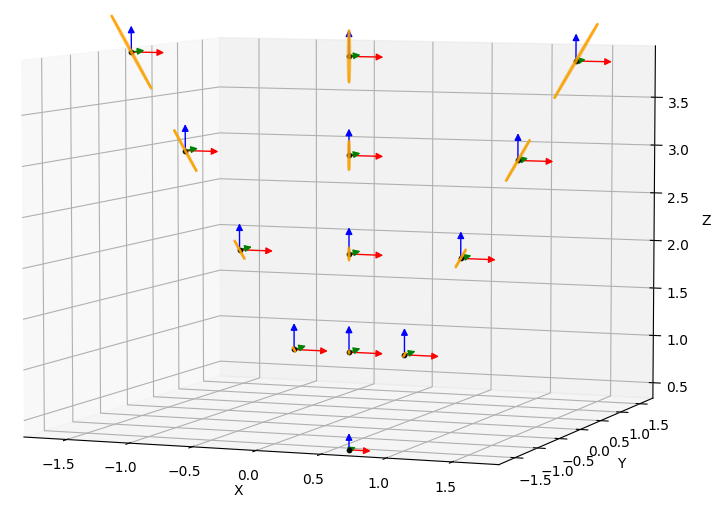
\includegraphics[width=\textwidth]{figures/apriltag_cov_posi.png}
        \caption{Relative position covariances \label{fig:apriltag_cov_posi}}
    \end{subfigure}%
    \hfill
    \begin{subfigure}{.49\linewidth}
        \centering
        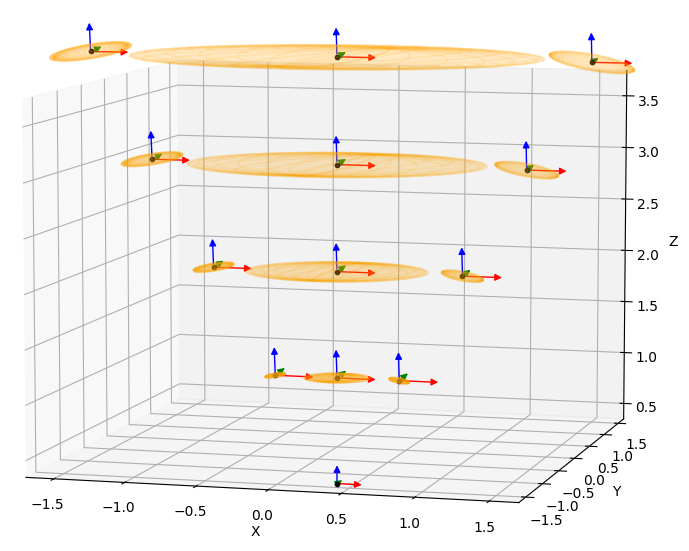
\includegraphics[width=\textwidth]{figures/apriltag_cov_orientation.png}
        \caption{Relative orientations covariances \label{fig:apriltag_cov_orientation}}
    \end{subfigure}%
    \caption{Representation of the analytic covariance model. The single frame at the bottom represents the pose of the virtual camera, others are identical 
    \apriltags placed in front of the camera at different distances but identical orientations, covariances are represented in orange, centered at the corresponding tag position.
    (\subref{fig:apriltag_cov_posi}) shows that the main positional uncertainty is along the camera-tag axis, which corresponds to the distance information. 
    (\subref{fig:apriltag_cov_orientation}) shows that in contrary the rotation along the camera-tag axis is by far the most precise.}
    \label{fig:apriltag_cov}
\end{figure}

We can see that the error distribution is clearly anisotropic. The uncertainty of the pose measurements
is logically higher in the dimensions that lead to the least change in the aspect of the tag projection. For a fronto-parallel tag, the highest 
uncertainty is along the z-axis, which corresponds to a high depth uncertainty.
In \figRef{fig:apriltag_proj}, 3 tags are projected: the first (black) is half a meter away from the camera in fronto-parallel orientation, the second (orange)
10cm to the right, and the third (rose) 10cm behind. We can see that the appearance of difference of appearance due to a depth-wise movement is much smaller, which 
explains the higher uncertainty on the depth measurement. Similar reasoning can be made for orientation as well. 

\begin{figure}[h]
    \centering
    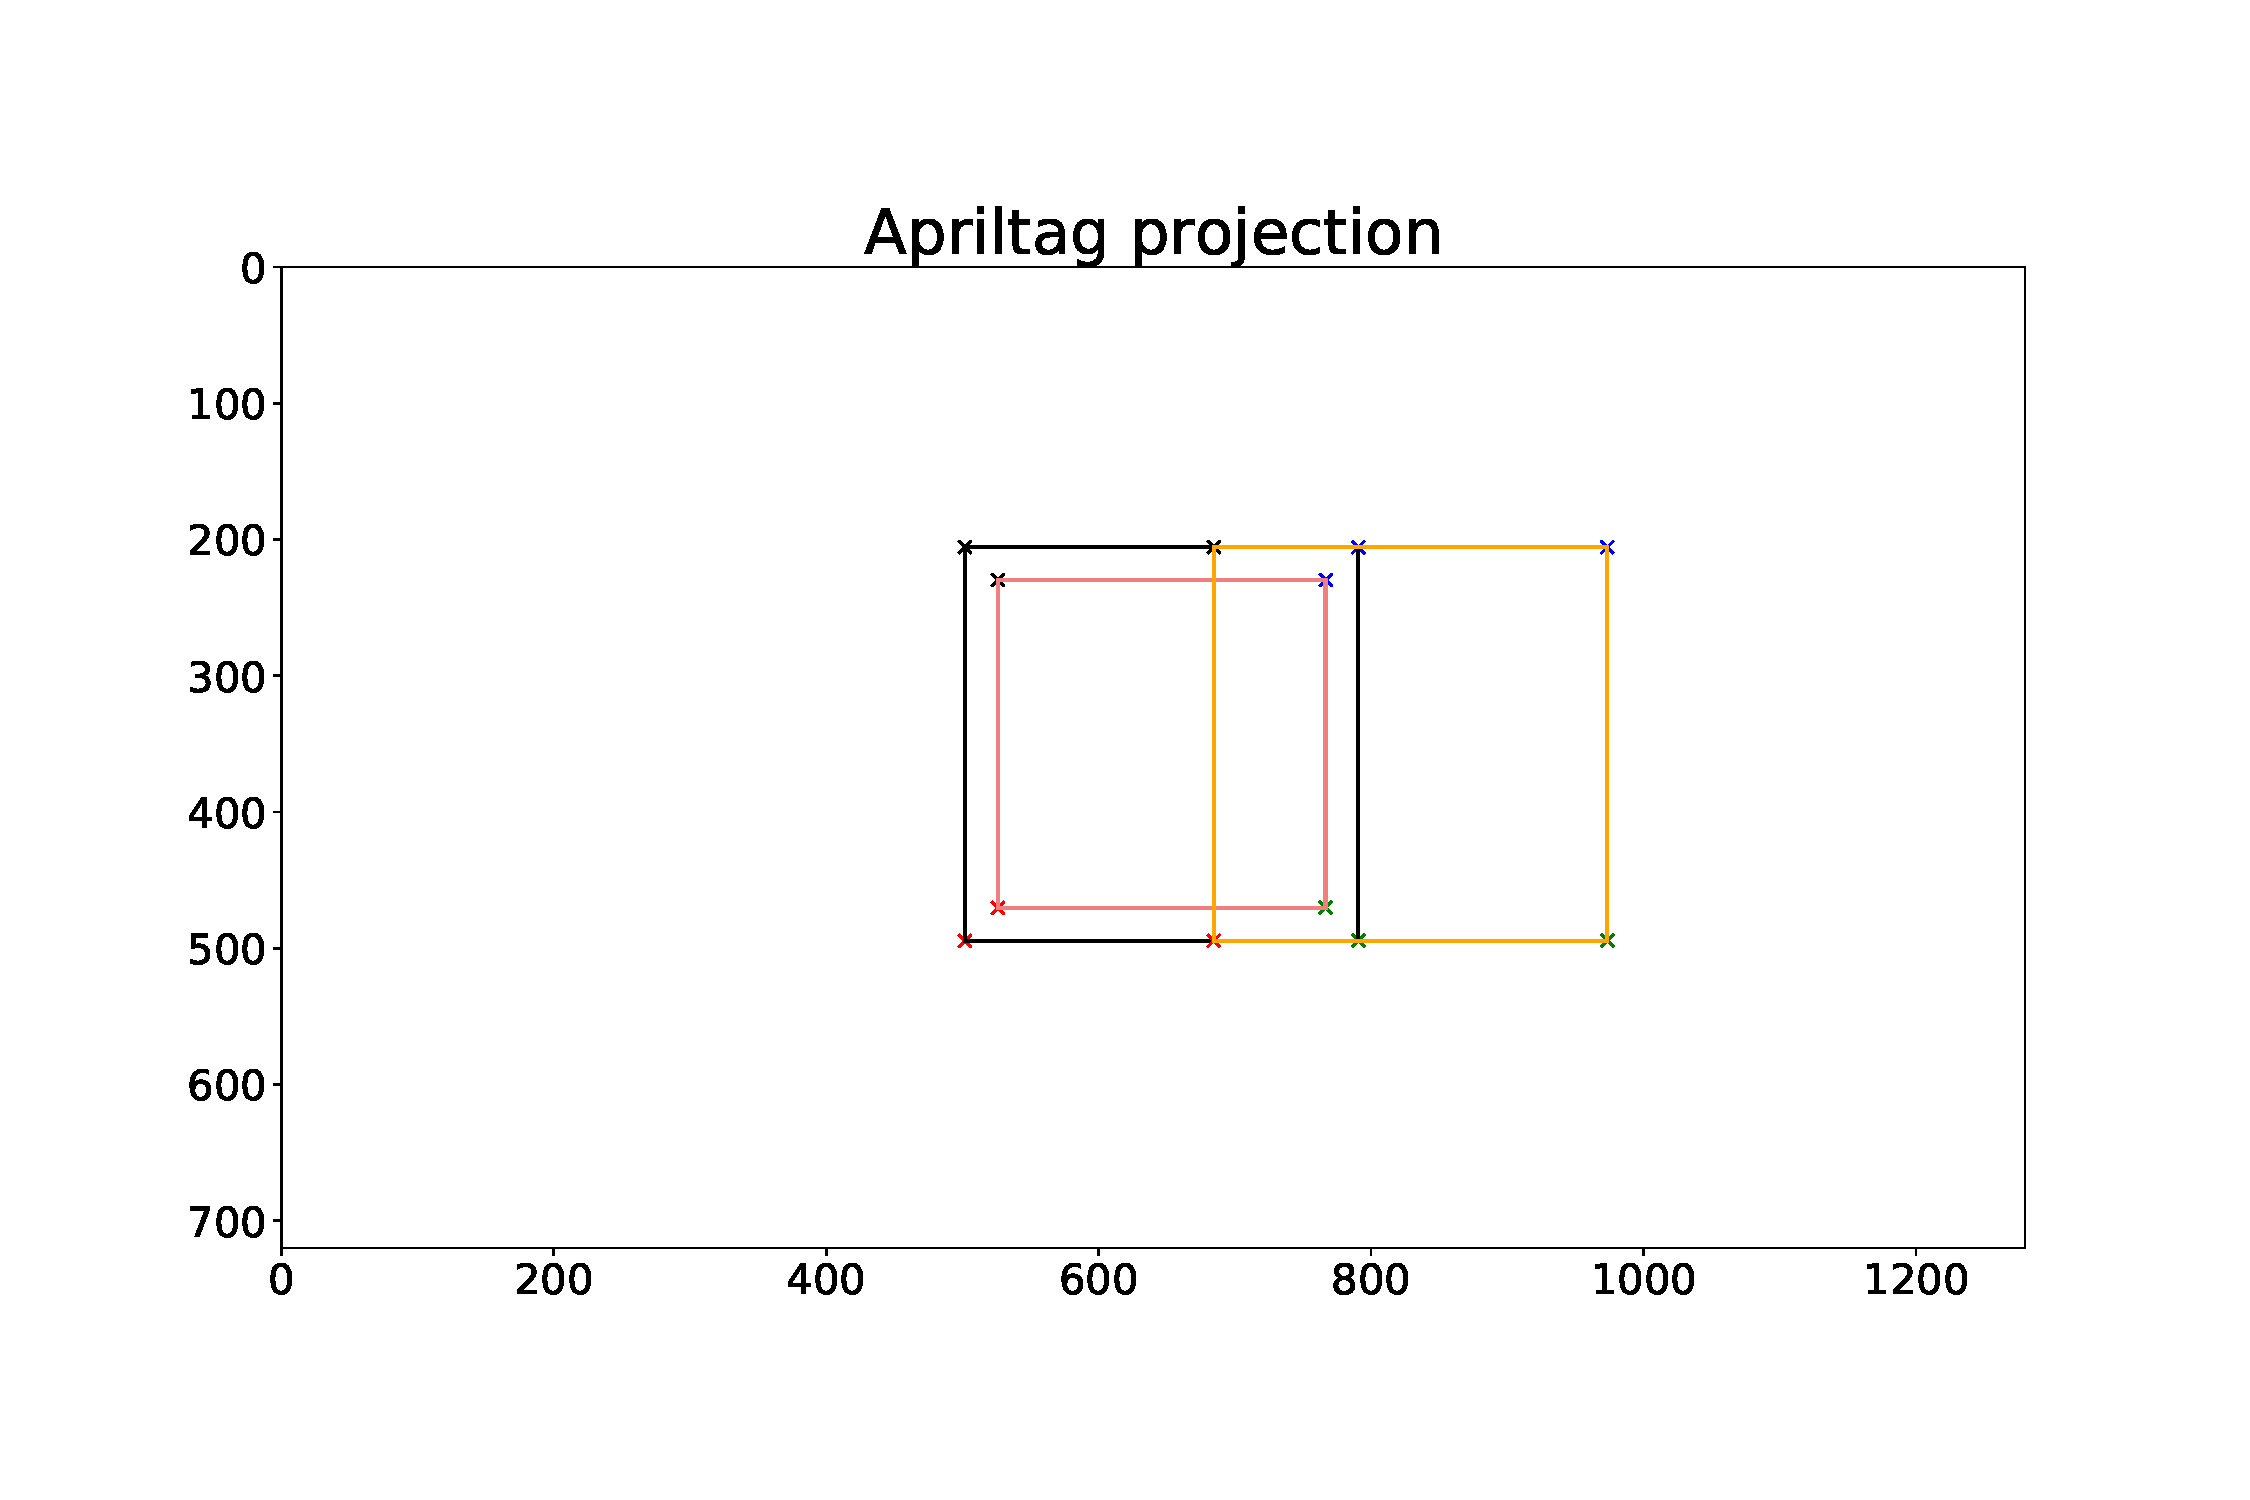
\includegraphics[width=0.8\textwidth]{figures/apriltag_proj.pdf}
    \caption{Projection of 3 tags of camera frame position: black -> (0,0,0.5), orange -> (0.1,0,0.5), rose -> (0.0,0,0.6)}
    \label{fig:apriltag_proj}
\end{figure}

A quantitative comparison with \cite{urban2016mlpnp} would be interesting as well as an experimental validation campaign.


\subsection{Ambiguity in the pose estimation}
It is well known that the pose extraction from planar markers suffers from an inherent ambiguity between two fairly different rotations as described in 
\cite{8206468} for instance. One solution is to define the tag factor residual as the pixel error between the detected corners and their projection given the
current tag pose estimate and let the optimizer find the most probable tag poses given the complete set of measurements. However if one tag is wrongly initialized, 
the optimizer is not guaranteed to leave the local minimum with new measurements. Our solution is to bring the disambiguation to the front-end side.
\cite{collins2014infinitesimal} provides an implementation of the PnP problem that retrieves both ambiguous poses. When expressed in the camera frame, 
both solutions share the tag position and differ only in their orientation. We typically want to select the solution with the smallest error. 
However, if the reprojection errors $e_1$ and $e_2$ are too close (we test for $\tfrac{e_2}{e_1} < h$ with $e_1 \leq e_2$ and $h$ an empirical threshold), 
we increase the rotational part of the covariance matrix by a great factor to prevent a potential wrong tag orientation to influence the estimation.


Necker's cube









%
%
%
%
\section{Learning-based object pose estimation}
In this section, we propose to integrate a deep-learning-based object pose estimation algorithm \cite{labbe2020cosypose} to our measurement models. 


\subsection{Object pose estimation algorithms}
\label{sec:object_pose_est}
The problem of object pose estimation can simply be stated: given a calibrated camera and a set of known object models, detect those objects in the current image 
frame and extract camera-objects poses. Traditionally, competing methods were developed using either local features matching or learning-based methods.
As shown by the most recent BOP challenge results \cite{hodan2020bop}, deep-learning methods now clearly dominate the field in terms of accuracy. 
At the time of the writing, the highest-ranking non-learning-based pose extraction method \cite{konig2020hybrid} (object detection is deep learning-based) 
actually uses depth measurement measurements and is dominated by a purely RGB, deep-learning-based model \cite{haugaard2021surfemb}, though \cite{konig2020hybrid} 
seems to be ten times faster \footnote{BOP challenge leaderboard is available at \url{https://bop.felk.cvut.cz/leaderboards/}}.

In terms of accuracy, these results advocate for the use of deep-learning purely RGB image-based methods, that now provide accurate enough results 
for these to be used in robotics applications \cite{labbe2021single}. 
We use the CosyPose model of Labbe et al. \cite{labbe2020cosypose} which at the time ranked first in the BOP challenge leaderboard.
This approach mixes a new state-of-the-art single-view pose estimation algorithm with a multi-view algorithm using RANSAC and Bundle Adjustment. 
It achieved first in most of the 2020 BOP challenge categories \cite{hodan2020bop}. This system obtains precision in the order of centimeters 
on real objects whose 3D model is known. Its performances make it a good candidate as a direct 6D pose sensor to perform a multi-sensor fusion. 
In the context of legged robots, this is very useful to localize the robot relative to objects it needs to interact with, such as objects 
to manipulate or stairs to climb. While CosyPose is not yet able to generalize to unseen classes of objects, rapid progress is expected in 
this direction.

\subsection{CosyPose}
The front end of the SLAM system designed for this project includes object detection and object pose estimation. 
This function is provided by CosyPose \cite{labbe2020cosypose}, a deep learning-based 6D pose estimator that reaches state-of-the-art
 performances for 6D object pose estimation. % and which was awarded at the BOP contest \cite{hodan2020bop}. 
In the original paper, a single-view pose estimator and a multi-view algorithm were introduced. In our context, only the single-view module is used, 
while object tracking is handled by the SLAM framework. 

CosyPose takes as input a single image $I$ and a set of 3D models, each associated with an object label $l$. The camera $C$ is assumed to be calibrated. 
A set of object detections is performed using the object detector Mask-RCNN \cite{he2018mask}. Each 2D candidate detection is identified 
by an index $\alpha$ and associated with an object candidate $O_{\alpha}$. Its 6D pose $\T{C}{O_{\alpha}} \in \SE (3)$ relative to the camera $C$ 
is then computed as follows.

\begin{figure}[]
    \begin{subfigure}{.5\textwidth} % this sets the figure to be max half the width of the page
        \centering
        % include first image
        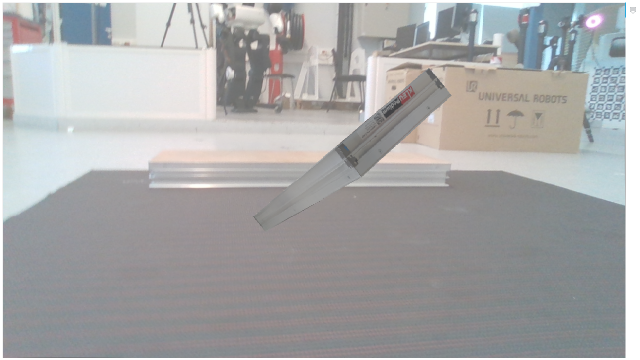
\includegraphics[width=.9\linewidth]{figures/cosyslam/convergence_1.png}  % this sets the image to fill 90% of the available space -> 45% of the line width in total. 
        % \caption{\label{fig:cosypose-convergence_1}}
    \end{subfigure}
    \begin{subfigure}{.5\textwidth}
        \centering
        % include second image
        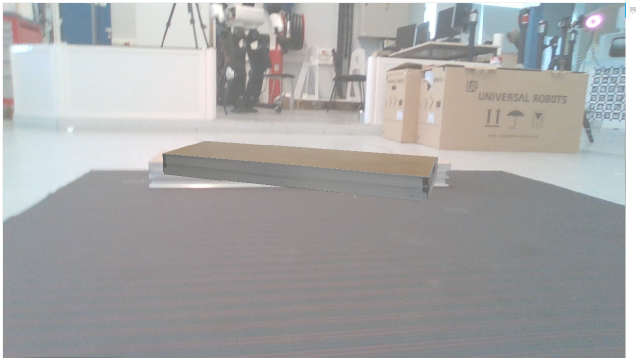
\includegraphics[width=.9\linewidth]{figures/cosyslam/convergence_2.png}  
        % \caption{\label{fig:cosypose-convergence_2}}
    \end{subfigure}

    \label{fig:fig}
    \begin{subfigure}{\textwidth}
        \centering
        % include first image
        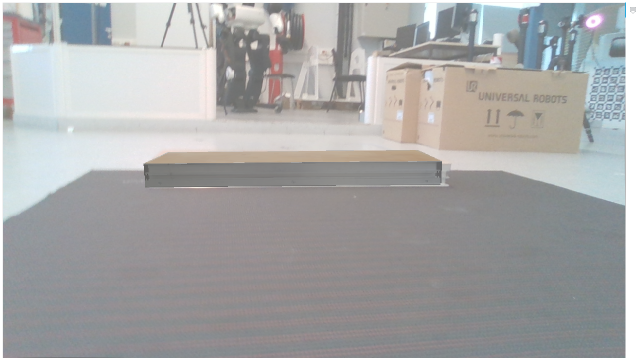
\includegraphics[width=.45\linewidth]{figures/cosyslam/convergence_3.png}   % this width should be half of the width of the other two images
        % \caption{\label{fig:cosypose-convergence_3}}
        
    \end{subfigure}
    \caption{\label{fig:cosypose-convergence} Progressive convergence of a stair step estimated pose over successive iterations of CosyPose.}
\end{figure}


The single-view pose estimation procedure of CosyPose is an improvement over the one proposed in DeepIm \cite{deepim_2019}. The general idea is to iteratively 
use the same neural network to iteratively converge to the object pose (\figRef{fig:cosypose-convergence}). It takes as input the cropped image  of the detected 
object bounding box and a rendered image based on the current object pose solution $\T{C}{O_{\alpha},k-1}$ at iteration $k-1$. 
It returns a transformation update $\T{O_{\alpha},k-1}{O_{\alpha},k}$ that brings the rendered image closer to the cropped image. In practice, 
two neural networks with the same structure are trained independently: one for coarse pose estimation, \ie, the first iteration of the iterative process, 
and another for the refinement of the pose. The coarse network gives the first transformation $\T{C}{O_{\alpha},0}$, 
and the prediction of the pose of the object is obtained by composing the $N$ successive transformations:

\begin{equation}
\T{C}{O_{\alpha}} = \T{C}{O_{\alpha},0} \prod_{k=1}^N  \T{O_{\alpha},k-1}{O_{\alpha},k}.
\end{equation}

CosyPose reuses the neural network architecture of DeepIm with a new backbone for feature extraction, Efficient-Net \cite{tan2020efficientnet} ,
with a spatial average pooling layer added after it. Then, it disables the optical flow sub-network during the training. 
A new rotation parametrization, introduced in \cite{zhou2020continuity}, is used for the loss function, which has been shown 
to bring more stability during training. Then, the focal length of the cropped images is recomputed during training to fit the virtual camera 
of these images. Finally, the object symmetries are taken into account during training thanks to the \textit{symmetric distance}. 
Each 3D model $l$ is associated with a set of symmetries $S(l)$, that is the set of transformations that leave the aspect of the object unchanged:

\begin{equation}
    \textit{S}(l) = \left \{ \bfS \in \SE(3) | \forall \bfT \in \SE(3), \cR(l,\bfT) = \cR(l,\bfT \bfS)\right \}
\end{equation}
%
where $\cR(l,\bfT)$ is the rendered image of the object $l$ captured in pose $M$. Given a set of symmetries $S(l)$, 
the symmetric distance $D_l$ measures the distance between two 6D poses represented by transformation $\bfT_1$ and $\bfT_2$. 
Given an object $l$ associated to a set $\cX_l$ of 3D points $\mathbf{x} \in \cX_l$, we have:

\begin{equation}
    D_l(\bfT_1, \bfT_2) = \underset{\bfS \in \textit{S}(l)}{\text{min}} \frac{1}{|\cX_l|} \sum_{\mathbf{x} \in \cX_l} ||\bfT_1 \bfS \mathbf{x} - \bfT_2\mathbf{x} ||^2.
    \label{eq:distSym}
\end{equation}

Equation \eqRef{eq:distSym} measures the average distance between the points of the object model transformed by $\bfT_1$ and $\bfT_2$ according to the symmetry 
that best aligns the transformed points. In practice, for continuous symmetries  that are rotations around an axis (like for instance for a textureless cylinder), 
$S(l)$ is discretized using 64 angles.


\subsection{Empirical covariance estimation}
\label{sec:cosypose_covariance}

When considering merging a tracker such as CosyPose with other sensor modalities, an important aspect is to predict covariance representing the level 
of confidence in the tracker estimate. Such data uncertainty is crucial to the robustness of SLAM systems involving neural networks 
subsystems such as \cite{yang2020d3vo}. The depth-based object SLAM algorithm \cite{SalasMoreno2013SLAMSL} claimed to compute a covariance matrix approximated 
as the inverse of the Iterative Closest Point output. The methods targeted for deep learning applications are harder to implement, especially if the goal 
is to use an off-the-shelf pose estimation neural network, as is the case for this paper. For instance, Bayesian Neural Networks \cite{jospin2020hands} 
need to be trained explicitly for uncertainty prediction while Monte Carlo (MC) Dropout \cite{gal2016dropout} requires multiple forward passes at run-time.

In our work CosySLAM \cite{debeunne2021cosyslam} (submitted at ICRA22), we present a practical implementation of a SLAM system based on the design of an off-the-shelf deep learning object 
pose estimation algorithm \cite{labbe2020cosypose}, which empirical results are presented in \chpRef{chp:cosyslam}. 
To integrate these measurements with other sensors, we propose a noise model based on empirical data.

\subsubsection{Covariance model}

CosyPose does not provide an evaluation of its uncertainty.
%
The two main families of solutions available to estimate uncertainties of neural network predictions consist in MC dropout \cite{gal2016dropout} 
or Bayesian Neural Network (BNN) \cite{jospin2020hands}. Using BNNs would require changing the architecture of CosyPose and retraining it. 
MC dropout would require several forward passes through the network for each iteration, which would be computationally expensive. 

We need to compute the covariance without changing the architecture of the network and at an affordable cost. 
We propose to make an empirical error model based on polynomial regression in order to compute the covariance matrix. 
The idea is to parametrize the average error on each $\se(3)$ component returned by CosyPose. We conduct an empirical study on several video 
sequences that explore the variations of the parameter set for several object types. The error is computed by comparing the $\SE(3)$ transformations 
between the camera $C$ and an object $O$ returned by CosyPose $\T{C}{O}$ with the same transformation given by a motion capture system. 
We then use the error predictions of our parametric model as a proxy to the true 6 covariances during model fitting. 
A different model is fit for each object type due to their diversity of shapes, sizes, and textures.

The parameters used to compute the error need to represent the error sources of CosyPose as much as possible. 
To cover the error due to the configuration of the object in space, we need to include the 3D coordinates of the camera in the object frame. 
We also want to take into account some invariance that can occur by rotating around the object if it is texture-less for example. 
For this reason, we choose spherical coordinates of the camera origin with respect to the object frame to parametrize the model. 
Another source of error can be the occlusion of the object in the scene, as well as the motion blur, or any inherent noise in the image. 
This can affect the quality of the detection and of the pose estimation. Mask-RCNN returns a confidence score $s$ for each detection 
that we will include in our model. This score is the output of the final softmax layer of the detector and can be interpreted
as the level of confidence Mask-RCNN has in its prediction.

% To sum up, we have the following parameters for our error model:
% \begin{itemize}
% \item $\displaystyle r = || \posihat{O}{C}||$,
% \item $\displaystyle \varphi  = \arctan\left(\frac{ \prescript{0}{}{\hat{x}}_C}{\prescript{0}{}{\hat{y}}_C}\right)$,
% \item $\displaystyle \theta  = \arcsin\left(\frac{\prescript{0}{}{\hat{z}}_C}{r}\right)$,
% \item $\displaystyle s$ : mask-RCNN softmax output.
% \end{itemize}

To sum up, our model is parametrized by four values: $r$ - distance, $\varphi$ - azimuth, $\theta$ - elevation, $s$ - Mask-RCNN softmax output. 
We can then compute the error of CosyPose relative to the motion capture data: 

\begin{equation}
    \mathbf{e}  = [\mathbf{e}_{t}, \mathbf{e}_{a}]  \triangleq  \left[~\posihat{O}{C} - \posim{O}{C}, ~ \Log \left(\Rothat{O}{C}^{-1}\Rotm{O}{C}\right)~\right]
\end{equation}
%
where $\widehat{\cdot}$ and $\widetilde{\cdot}$ denote quantities obtained from the motion capture system and CosyPose respectively. 
$\Log$ denotes the logarithm application mapping elements of SO(3) to the $\Reals^3$ representation of its Lie algebra 
$\so(3)$.

We want to find a polynomial function $f(r, \varphi, \theta, s) \in \mathbb{R}^6$ that returns the error given the set of training data $\{X,E\}$. 
For each object, we capture a set of video sequences and we compute the error with the motion capture data for each measurement. 
We then perform polynomial regression with a pipeline in Scikit Learn \cite{scikit-learn}. A simple linear regression leads to a high root-mean-square error (RMSE) 
on a test dataset. Over degree 3, the model overfits and the high curvature of the polynomial returned high error values outside of the training data range. 
Thus, a degree 2 polynomial regression seemed to offer a good compromise.  Quantitative results are given in the experimental validation section 
(see Fig.~\figRef{fig:empirical_err} for a few examples of fitted polynomials).







\subsubsection{Empirical covariance}

As explained in Sec. II, we have trained empirical models to evaluate the covariance of the estimation of CosyPose. 
To validate these models, we propose to exhibit a few intuitive observations and a quantitative statistical analysis. 
One of the parameters involved in our model is the absolute distance between the camera and the object, noted $r$. 
Our trained models show an expected behavior regarding this parameter: the global error increases when the camera moves away from the object. 
%
\begin{figure}[h]
  \centering 
  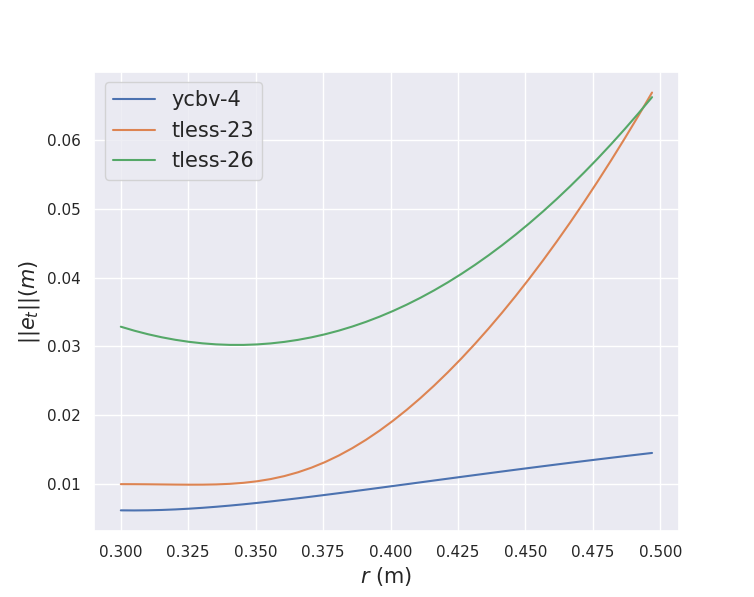
\includegraphics[width=0.8\textwidth]{figures/cosyslam/empirical_err.png}
  \caption{The norm of the translation error returned by the models of three different objects with respect to $r$, the distance between the camera and the object. 
            The other parameters $\theta$, $\phi$ and $s$ are fixed to the average values of our training data. }
  \label{fig:empirical_err}
\end{figure}

\figRef{fig:empirical_err} sheds light on these phenomena and gives an explicit comparison between the models of different objects. 
The error of the object from the YCBV dataset seems more stable and smaller than the one of the objects from the T-LESS dataset. 
This can be explained by the texture of the object and the absence of symmetries: T-LESS objects are known to be more challenging 
for pose estimation and this is confirmed by our model.

A more quantitative evaluation can be deduced from table \tabRef{table:empirical_models}. The translation error seems to be captured pretty well,
 as the RMSE is around the centimeter. However, the angular error seems a little less predictable, especially for T-LESS objects whose orientation 
 estimation can suffer from an important measurement noise due to the lack of textures. The $R^2\in[0,1]$ score is the coefficient of determination 
 and is often used to evaluate statistical models. Its interpretation is subject to debate and cannot conclude by itself on the absolute quality of model. 
 However, a score higher than 0 demonstrates that the model is more accurate than a baseline average model.

\begin{table}[h]
    \centering
    \begin{tabular}{|c|c|c|c|}
        \hline 
          & $\displaystyle R^{2}$ & RMSE ang. err. (°) & RMSE trans. err. (cm) \\
        \hline 
         YCBV-4 & 0.55 & 5,1 & 0.6 \\
        \hline 
         T-LESS-23 & 0.5 & 11.7 & 1.5 \\
        \hline 
         T-LESS-26 & 0.68 & 22 & 0.6 \\
         \hline
    \end{tabular}
    \caption{A quantitative evaluation of our models, these values are computed on test samples that were not used for training. }
    \label{table:empirical_models}
\end{table}



\subsection{Retraining with stairs}
\label{sec:retraining_with_stairs}
In order to produce a realistic SLAM scenario in the context of legged robots, we retrained CosyPose with staircases present in our lab.
We made a textured mesh of a stair step used in our experimental platform. This textured mesh was used both for training and using the trained model. 
The generation of photorealistic synthetic data was handled by BlenderProc \cite{denninger2019blenderproc}. The render-and-compare loop uses PyBullet \cite{coumans2021}.

\begin{figure}[h]
    \centering
    \begin{subfigure}[]{{.33\linewidth}}
        \centering
        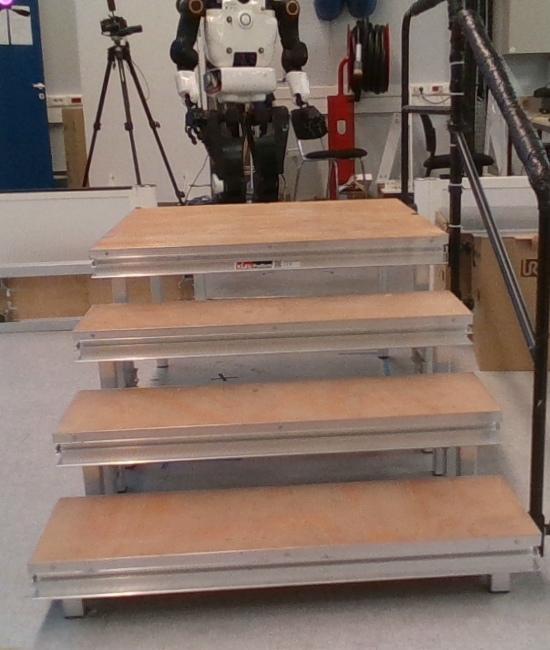
\includegraphics[width=\textwidth]{figures/cosyslam/0006.png} 
    \end{subfigure}
    \hspace{2cm}
    \begin{subfigure}[]{{.33\linewidth}}
        \centering
        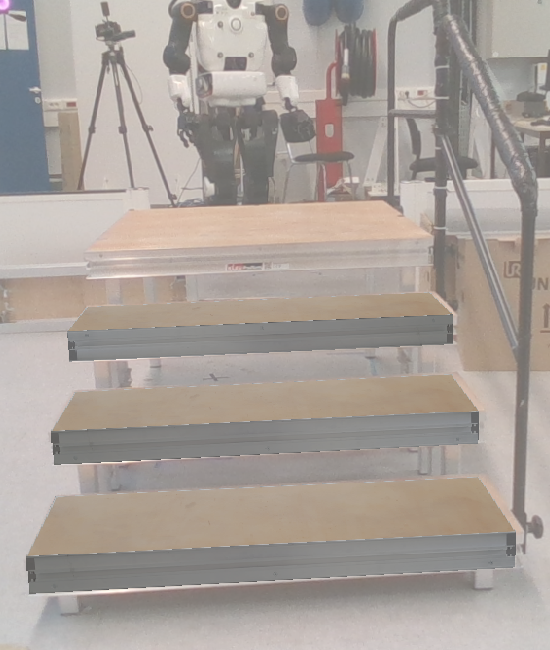
\includegraphics[width=\textwidth]{figures/cosyslam/0006_proj.png} 
    \end{subfigure}
    \caption{On the left, a picture of our climbing module at LAAS and on the right the 3D model of the stair projected according to CosyPose measurements on the same picture}%
    \label{fig:cosypose-ycbv}%
\end{figure}

We generate 10.000 synthetic images that are labeled with object pose ground truths. We retrain the three modalities of CosyPose: 
the Mask-RCNN detector, the coarse pose estimator, and the pose refiner. We slightly tune the training parameters used for the object from the BOP challenge as 
the scale is different: the stair is $1m \times 0.3m \times 0.07m$ whereas a T-LESS object is never wider than $10cm$. 
Thus, we generate training data on $10m \times 10m$ scenes, and we increase the noise used to train the refiner.  

An illustration of the performances of CosyPose on a set of 3 stair steps is given on \figRef{fig:cosypose-ycbv}: 
the pose of each step is here independently estimated which leads to local accuracy but global inconsistency. 
%\chapter{Kinematics}
\minitoc
\bigskip

The robot kinematic model along with encoder measurements make possible the computation of poses and spatial velocities \cite{featherstone2014rigid} (aka. twists) 
of reference frames attached to the robot segments relative to the base or world frame. This kinesthesis capability is of paramount importance to control
multi-body systems for locomotion or other interactions with their environment. If we have information about stable contacts that the robot keeps with
its environment, it is possible to infer a relative motion measurement, which is commonly called leg-odometry.

We will shortly describe the formulation of the forward-kinematics algorithm, that enables to compute relative poses and spatial velocities between parts of the robot
and then show how this information can be used to define a leg-odometry factor to be added in the factor graph. The last section shows how forward-kinematics can also be used to leverage prior 
information about the height of the environment. 



\section{Forward kinematics}
\label{sec:forward_kinematics}
We first describe the forward-kinematics and differential kinematics algorithms by introducing notations commonly found in the legged robots literature.

The degrees of freedom (DoF) $n$ of a poly-articulated system is the minimal number of variables that completely describe his state given the base frame. 
For robots with rigid segments, the DoF of the robot is the sum of the DoFs of its joints (1 for linear and rotational joints, 3 for
ball joints, etc.).
The state of the joints (1 angle for rotational joints) can be stacked together in the vector of joint configurations 
$\qa \in \Reals^n$. For most simple joints, the joint configuration velocities are simply the time derivative $\dqa \in \Reals^n$\footnote{An exception is the ball joint where the 
state is defined as an element of $\SO(3)$, thus its velocity vector is defined as an angle axis in $\Reals^3$.}. $\qa$ and $\dqa$ are typically obtained from
the joint encoder measurements.
Legged robots are not fixed to the ground so we add a so-called "free-flyer" FoF which represents the free pose of the base with respect to the world and is modeled as an 
unactuated joint of 6 DoF pertaining to the $\SE(3)$ group. Its velocities are therefore in the $\se(3)$  Lie algebra, isomorphic to $\Reals^6$. 

The whole-body state of the robot is defined by the robot configuration vector $\bfq=[\bfq_b,\qa]\in \SE(3) \times \Reals^n$, where 

\begin{equation}
    \bfq_b \triangleq \T{W}{B} =  
    \begin{pmatrix}
        \Rot{W}{B} & \posi{W}{B} \\
        \bf0_3\tr & 1
    \end{pmatrix}
\end{equation}
%
is the configuration of the base,
with $\posi{w}{b} \in \Reals^3$ and $\Rot{W}{B} \in \SO(3)$ are the position and orientation of the base with respect to the world.
$\qa \in \Reals^n$ is the configuration of the joints. $\bfq$ therefore belongs to a composite manifold $\cM_{\bfq} = \left<\SE(3), \Reals^n \right>$ and 
the configuration velocity vector belongs to its tangent space $\se(3)\times \Reals^n$ which is isomorphic to $\Reals^{6+n}$: $\bfv_q \in \Reals^{6+n}$. Those are concatenations
of the base state and joint configuration vectors:
%
\begin{equation}
    \bfq= [\bfq_b, \qa]\in \cM_{\bfq}\quad\quad,
    \quad\quad
    \bfv_q= [\prescript{b}{}{\mathbf{\nu}}_b,\dqa]  \in \Reals^{6+n}
    \label{eq:configuration}
\end{equation}
%
where $\prescript{b}{}{\mathbf{\nu}}_b$ is the twist of the base frame expressed in the base frame.
The computation of any segment pose of index $k$ relative to the world is obtained using the forward-kinematics (FK) algorithm:
%
\begin{equation}
    \T{W}{K} = \text{FK}_k(\bfq).
\end{equation}

The kinematic chains of most robots can be represented as a tree whose root is the world frame, nodes are the joints to which are associated reference frames 
(including the base, which is considered as a $\SE(3)$ joint), and edges are solid segment placed between these nodes.
The forward-kinematics algorithm consists of a forward pass from the root of the tree $\T{W}{B}$ through the joints along the path to the leaf $\T{W}{K}$ that we wish to obtain. 
Let us denote by $i$ the index of each intermediate joint between the root and the leaf, the root (world) having index 0 and the base index 1, 
the forward-kinematics algorithm simply writes as a composition of successive transformations:

\begin{equation}
    \Tbar{0}{k} = \T{0}{1}(\bfq_b) \Tbar{1}{2'}
    \T{2'}{2}(q_2) \dots  \Tbar{k-1}{k'} \T{k'}{k}(q_k)
\end{equation}
%
where $\Tbar{i-1}{i'}$ designates the transformation between joint frames $i-1$ and $i$ when the joint configuration $q_i$ is at the identity value and is a constant. 
The $\T{i'}{i}(q_i)$ designate transformations caused by a non-zero joint value $q_i$, as reprsented in \figRef{fig:forward_kinematics}.

\begin{figure}
    \centering
    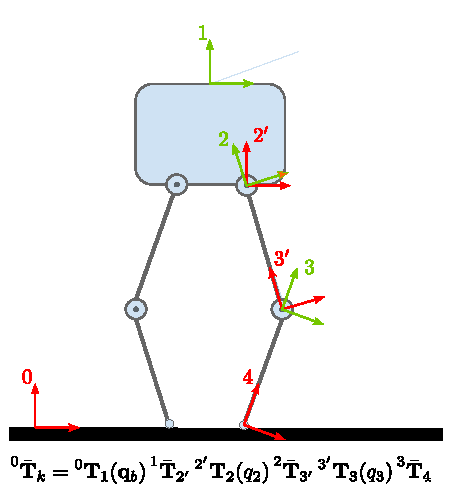
\includegraphics[width=0.5\textwidth]{figures/kinematic_tree_FK.pdf}
    \caption{Illustration of the Forward kinematics algorithm to get the transformation of the foot $4$ with respect to the world $0$.}
    \label{fig:forward_kinematics}
\end{figure}


It is also possible to obtain the pose relative to the base $\T{b}{k}$ by simply setting the base pose vector to be the identity pose $[0,0,0,~0,0,0,1]$.

% Differential FK is not used anywhere so...
% FK is a nonlinear function of the robot configuration. 
% To obtain the relative spatial velocity, we have to compute the Jacobian $\bfJ_k$ of FK with respect to the configuration.
% The differential forward-kinematics (DFK) is then simply:

% \begin{equation}
%     \prescript{w}{}{\mathbf{\nu}}_k = \bfJ_k \bfv_q    
% \end{equation}

Similarly, the spatial velocity relative to the base $\prescript{b}{}{\mathbf{\nu}}_k$ can be obtained by setting the base spatial velocity part of $\bfv_q$ to zero.
These algorithms are very fast to compute ($\approx 1\mu s)$ using modern dedicated libraries \cite{carpentier2019pinocchio}.

We will now see how FK can be used to derive leg-odometry for a quadruped robot.

\section{Leg odometry}
\label{sec:leg_odometry}
We will restrict ourselves to the case of point feet as the main platform on which we experimented is a quadruped robot.
Quadrupeds are usually equipped with non-articulated round feet whose contact with the ground is, in first approximation, punctual.
Humanoid robots are equipped with articulated flat feet that provide richer information. In \secRef{sec:kinematic_info} we gave an exhaustive review of the types of leg 
odometry measurements that can be obtained on legged machines.

The basic idea is that we assume to have access to accurate contact detection. If the contact is held between time $t_i$ and $t_j$ and that
the contact point $L$ (to which a frame is attached) is fixed. This can be written $\posi{W}{L}^i = \posi{W}{L}^j$. 
In practice, the round feet of our robot can slightly roll but we will neglect this phenomenon. 
If we unfurl the transformation chain to make the base poses appear in the equation, we obtain the identity:

\begin{equation}
    \posi{}{}^i + \Rot{}{}^i \posim{B}{L}^i = \posi{}{}^j + \Rot{}{}^j \posim{B}{L}^j
\end{equation}

We can immediately derive the residual $\bfe^{LO}$ expression for each foot $l$ in contact between $t_i$ and $t_j$:

\begin{equation}
    \bfe^{LO}_l(\posi{}{}^i, \Rot{}{}^i, \posi{}{}^j, \Rot{}{}^j) = \posi{}{}^i + \Rot{}{}^i \posim{B}{L}^i - (\posi{}{}^j + \Rot{}{}^j \posim{B}{L}^j)
\end{equation}

To obtain a proper measurement model, we need to model the influence of measurement inaccuracies.
This equation depends on relative positions $\posim{B}{L}^i$ and $\posim{B}{L}^j$ that are computed using FK. The quality of the computation depends on several things:
the robot kinematic model (calibration), deviations from the rigid body model (\eg segment/joint flexibilities, backlash), encoder noise.
It is tempting to propagate encoder noise $\noise_{\qa}$ through FK using the kinematic Jacobian \cite{bloesch2013state, hartley2018legged}:

\begin{equation}
    \posim{B}{L} = FK(\qa + \noise_{\qa}) \approx FK(\qa) + \bfJ_L\noise_{\qa}, \quad \quad \Cov_{p} = \bfJ_L \Cov_{\qa} \bfJ_L
\end{equation}

However, the resolution of Solo encoders is very high: 0.002 degrees, which would account for a mere 10 \textit{micrometers} difference.
Therefore, most of the measurement errors come from the other mentioned effects. Unfortunately, those are much harder to model, and all act at the same time
in an unpredictable fashion. Thus, we opt for a simple additive noise on the foot position in the world:
%
\begin{equation}
    \posi{W}{L}^i = \posi{W}{L}^j + \noise_{LO}
\end{equation}
%
where $\noise_{LO} \sim \Gaussian{0}{\Cov_{LO}}$ denotes a Gaussian noise accounting for potential roll/slip of the foot and kinematic inaccuracies.
This noise can be modeled as white noise on the foot velocity $\noise_v$, which when integrated gives a random walk.  
Its variance after $\Dt$ is 
%
\begin{equation}
    \Cov_{LO} = \Dt \Cov_v
\end{equation}
%
where $\posim{B}{L}^i$ and $\posi{B}{L}^j$ are the contact positions in base frame at times $t_i$ and $t_j$ acquired from $\qa$ via forward-kinematics. 
The residual errors $\bfe^{LO}_l$ and their covariances can be added as factors to the factor graph that we wish to build.

In the literature review and \figRef{fig:kin_models}, this method is referred to as \textit{single foot matching}. To obtain
a relative transformation of the robot's base frame between $t_i$ and $t_j$, at least three stable feet contacts are necessary. When it is the case, it is possible to directly compute the
relative transformation, which would be integrated as a separate residual, by solving an orthogonal Procrustes problem \cite{roston1991dead}.

However, for trotting gates common for quadrupeds, the robot is most of the time standing on only two legs, which makes the Procrustes problem computation rarely applicable. 
Instead, we add a single factor for each foot in stable contact. In fact, when at least 3 feet are in stable contact, the information extracted from these combined factors 
is the same as if we had pre-computed a 6D transformation from the Procrustes problem. Besides, when fusing with other sensors (such as the IMU,
see \chpRef{chp:centroidal_estimation}), 1 or 2 legs in contact already provide sufficient information to make the desired variables observable \cite{bloesch2013state}.



\section{Terrain height}
If we only use leg-odometry along with other sources of odometry such as an IMU (see \chpRef{chp:centroidal_estimation}, the position of the robot drifts after some time. 
However, if we have prior knowledge about the foot terrain height $h \in \Reals$, it is easy to define, for each foot $l$ in contact, the residual:

\begin{equation}
    \bfe^h_l(\posi{}{}, \Rot{}{}) = (\posi{}{} + \Rot{}{} \posi{b}{l})_z - h \quad, \quad e^{h}_l \in \Reals
\end{equation}

This residual can be assigned with a variance $\sigma_h^2$ which is hand-tuned. 
The error and its covariance form a unary factor (only depends on one \keyframe) that can be added to the factor graph we want to build.
Giving information about the height of the feet of the robot grounds the robot base height estimates and cancels the accumulation of drift in the vertical direction.






\section{Conclusion}

We have shown that leg odometry easily enters the MAP framework, using directly
the FK algorithms. This is a cheap and efficient way to express the meaningful contact
information in the factor graphs. As discussed in the state of the art, there are multiple
ways of formulating this information as an estimation factor. We have discussed
various possibilities and show why we have chosen the final formulation. There remains
some space to formally analyze this choice, possibly leading to a better formulation.
We will see in the last part of this thesis how it performs in practice.
Here we only considered the contact information as a motion constraint. We will
consider the resulting forces, ideally measured at the contact interface with a direct
force measurement device, to simultaneously estimate the basis state and the centroidal
quantities. But before that, we need to introduce the mathematics of pre-integration,
which we will first introduce in the context of the inertial measurements.

\chapter{High-rate motion data pre-integration}
\label{chp:preintegration}
\minitoc
\bigskip


Sensor modalities available on robotic platforms display a great variety in the rate at which measurements are acquired. For instance, 
a camera may record images at 33Hz while an IMU may be updated at 1kHz. In the context of Factor Graph estimation, this creates a challenge since residuals
are defined between \keyframes\ selected at a relatively low frequency, at times as low as 1Hz. One needs to integrate measurements from these high-rate sensors between \keyframes\,
which is not trivial in general.

In this chapter, we first describe the example of the integration of IMU measurements which motivates the development of the pre-integration theory \cite{lupton-09,forster2017-TRO}.
We then express this pre-integration in more abstract mathematical terms so as to generalize it to other high-rate sensors \cite{atchuthan-18-thesis}. 
Then, we describe a possible reformulation of the original IMU-preintegration algorithm \cite{forster2017-TRO} by exploiting a new Lie group that we 
proposed in \cite{fourmy2019absolute}. We conclude the chapter with a discussion of related works.

  
\section{A motivational example: IMU integration for graph optimization}
\label{sec:imu_preint_motivation}

In this section we will introduce the IMU measurement model and explain why a naive integration of these measurements in the world frame does not immediately
lead to a viable factor. We will then introduce the observations that lead to the development of the so-called IMU pre-integration algorithm by Lupton \cite{lupton-09}.

Let us consider the estimation of a robot base state comprised of its pose and velocity in the world frame,
%
\begin{equation}
    \bfx = [\posi{W}{WB}, \vel{W}{WB}, \Rot{W}{B}]
    \triangleq 
    [\bfp, \bfv, \Rot{}{}].
\end{equation}

We make a few hypothesis. First, we neglect effects due the rotation of the Earth by assuming 
that our world frame (which is fixed \wrt the ground) is an inertial frame. This is a common simplification in robotics scenarios \cite{forster2017-TRO}. 
Second, without loss of generality, we assume that the IMU frame is identical to the base frame in the following developments.

The IMU measurements are known to be noisy, biased, and affected by the gravity,
%
\begin{equation}
    \begin{split}
    \angvelm{}{} &= \angvel{B}{WB} + \bias_{\angvel{}{}} + \noise_{\angvel{}{}} 
    \\
    \accm{}{}    &= \acc{B}{WB} + \bias_{\acc{}{}} + \noise_{\acc{}{}} + \Rot{B}{W} \grav .
    \end{split}
    \label{eq:imu_meas_model}
\end{equation}
%    
Other sensors can help estimate the IMU biases $\bias \triangleq [\bias_{\acc{}{}}, \bias_{\angvel{}{}}]$ that are thus included in the estimator state.


Once the IMU has been started, these biases may change over time, more or less slowly depending on the quality of the IMU. This change is modeled 
as a random walk, which is close to the observed behavior for reasonably short periods of time \cite{hussen2015low}.
A dynamical model continuous-time based on strapdown integration of IMU measurements can then be derived:
%
\begin{align}
\begin{split}
    \dot{\posi{}{}} &= \vel{}{} \\
    \dot{\vel{}{}} &= \acc{W}{WB} \\
    \dot{\Rot{}{}} &= \Rot{}{} [\angvel{B}{WB}]_{\times} \\
    \dot{\bias}_{\bfa} &= \bfw_{\bfa}^c \\
    \dot{\bias}_{\angvel{}{}} &= \bfw_{\angvel{}{}}^c ,
\end{split}
\label{eq:imu_dyn_conti}
\end{align}
%
where $\bfw_{\bfa}^c \in \mathcal{N}(0,\bfW_\bfa^c)$ and $\bfw_{\bw}^c \in \mathcal{N}(0,\bfW_\bw^c)$ are the bias' random walk continuous-time white noises.

Introducing the measurement equations \eqRef{eq:imu_meas_model} in the continuous dynamics equations \eqRef{eq:imu_dyn_conti} and using a zero order hold
explicit Euler integration scheme during $\dt$ results in the discrete dynamics:
%
\begin{equation}
    \begin{split}
    \posi{}{}^{k+1} &= \posi{}{}^{k} + \vel{}{}^{k}\dt + \frac{1}{2}\grav \dt^2 
    + \frac{1}{2}\Rot{}{}^{k}(\accm{}{}^k - \bias_{\acc{}{}}^k - \noise_{\acc{}{}}^k)\dt^2 \\
    \vel{}{}^{k+1}  &= \vel{}{}^{k} + \grav \dt + \Rot{}{}^{k}(\accm{}{}^k - \bias_{\acc{}{}}^k - \noise_{\acc{}{}}^k)\dt
    \\
    \Rot{}{}^{k+1}  &= \Rot{}{}^{k}\Exp((\angvelm{}{}^k - \bias_{\angvel{}{}}^k - \noise_{\angvel{}{}}^k)\dt)
    \\
    \bfb_\bfa^{k+1} &= \bfb_\bfa^k + \bfw_\bfa\\
    \bfb_{\angvel{}{}}^{k+1} &= \bfb_{\angvel{}{}}^k + \bfw_{\angvel{}{}}
    \end{split}
    \label{eq:imu_dyn_disc}
\end{equation}
%
where $\bfw_{\bfa} \in \mathcal{N}(0,\bfW_\bfa)$ and $\bfw_{\bw} \in \mathcal{N}(0,\bfW_\bw)$ are the bias' random walk discrete-time white noises, satisfying $\bfW_\bfa=\bfW_\bfa^c \dt$ and $\bfW_\bw=\bfW_\bw^c\dt$.

    
Now, these equations relate consecutive states with data sampled at IMU frequency. To include these measurements in our smoothing estimator,
one solution would be to introduce new states at the rate of the IMU. However, the size of the problem would grow very quickly. A better option
is to integrate IMU measurements during extended periods of time. If we simply integrate the sequence of IMU measurements $\cZ_{im}$ between timestamps 
$t_i$ and $t_m$ by recursively applying \eqRef{eq:imu_dyn_disc}, we obtain:
%
\begin{equation}
    \begin{split}
    \posi{}{}^{m} &= \posi{}{}^{i} + \sum_{k=i}^{m} \Big[\vel{}{}^{k}\dt + \frac{1}{2}\grav \dt^2 
    + \frac{1}{2}\Rot{}{}^{k}(\accm{}{}^k - \bias_{\acc{}{}}^k - \noise_{\acc{}{}}^k)\dt^2 \Big] \\
    \vel{}{}^{m}  &= \vel{}{}^{i} + \sum_{k=i}^{m} \Big[\grav \dt + \Rot{}{}^{k}(\accm{}{}^k - \bias_{\acc{}{}}^k - \noise_{\acc{}{}}^k)\dt \Big]  \\
    \Rot{}{}^{m}  &= \Rot{}{}^{i} \prod_{k=i}^{m} \Exp((\angvelm{}{}^k - \bias_{\angvel{}{}}^k - \noise_{\angvel{}{}}^k)\dt) 
    \end{split}
    \label{eq:IMUIntij}
\end{equation}
%
where we assume that IMU biases stay constant during $\Dt^{im}$
\begin{equation*}
    \bias^k \approx \bias^i  ~~~ \forall k \in [i..m],
\end{equation*}
%
which makes their integration trivial and thus allows us to concentrate in the upper three lines of the model.




We are here in the position of illustrating why a naive definition of the data integration leads to very bad performance. 
By observing \eqRef{eq:IMUIntij} we can define a motion error, as follows. 
First, we naively define the motion increments or "deltas"
%
% \begin{equation}
%     \D_{im} = \left[\Dp_{im}, \Dv_{im}, \DR_{im} \right] \quad , \quad (\Dp_{im},\Dv_{im},\DR_{im}) \in \cM_{\D}=\left< \Reals^3,\Reals^3, \SO(3) \right>
%     \label{eq:delta_imu_def}
% \end{equation}
%
in two ways. 
%Note that delta quantities here belong to the composite Lie group $\left< \Reals^3,\Reals^3\in \SO(3) \right>$. 
From the integration of the motion model, %we get
%
\begin{align}
    \D_{im}(\bias^i, \bfx^i) = 
    \begin{bmatrix}
    \Dp_{im}\\ \Dv_{im}\\ \DR_{im}
    \end{bmatrix} \triangleq
    \begin{bmatrix}
    \sum_{k=i}^{m} \Big[\vel{}{}^{k}\dt + \frac{1}{2}\grav \dt^2 
    + \frac{1}{2}\Rot{}{}^{k}(\accm{}{}^k - \bias_{\acc{}{}}^i - \noise_{\acc{}{}}^k)\dt^2 \Big] \\
    \sum_{k=i}^{m} \Big[\grav \dt + \Rot{}{}^{k}(\accm{}{}^k - \bias_{\acc{}{}}^i - \noise_{\acc{}{}}^k)\dt \Big]  \\
    \prod_{k=i}^{m} \Exp((\angvelm{}{}^k - \bias_{\angvel{}{}}^i- \noise_{\angvel{}{}}^k)\dt)  
    \end{bmatrix}
    \label{eq:imu_delta_naive}
\end{align}
%
and from the difference between initial and final states:
%
\begin{align}
    \hat\D_{im}(\bfx^i, \bfx^m) = 
    \begin{bmatrix}
    \hat\Dp_{im}\\ \hat\Dv_{im}\\ \hat\DR_{im}
    \end{bmatrix} \triangleq
    \begin{bmatrix}
    \posi{}{}^{m} - \posi{}{}^{i} \\
    \vel{}{}^{m}  - \vel{}{}^{i}  \\
    \Rot{}{}^{i,T} \Rot{}{}^{m}  
    \end{bmatrix}.
\end{align}
%
Then, we build a residual error as
%
\begin{equation}
    \bfe(\bfx_i, \bfx_m, \bias_i) 
    = \D_{im}(\bias^i, \bfx^i) \ominus \hat\D_{im}(\bfx^i, \bfx^m) =
    \begin{bmatrix}
    \Dp_{im} - \hat\Dp_{im} \\ 
    \Dv_{im} - \hat\Dv_{im} \\ 
    \Log(\hat\DR_{im}\inv \DR_{im}) 
    \end{bmatrix}.
    \label{eq:error_naive_preintegration}
\end{equation}
%
where $\ominus$ is the composite manifold lift operator defined in \ref{eq:composite_retract}.

$\hat\D_{im}$ only depends on state variables and, thus, is cheap to compute. It corresponds to the "expected" motion of the system, given the current state estimates. 
$\D_{im}$ is the motion computed from the integration of (very many) IMU measurements during $\Dt_{im}$. However, since we "naively" integrated
in the world frame, this term also depends on the initial state $\bfx_i$ and on IMU bias $\bias_i$. This implies that for each update of the estimate $\bfx_i$, the IMU measurements need to be re-integrated from the new $\bfx_i$ and for the new $\bfb^i$. This is highly inefficient and, therefore, not well adapted to the repeated evaluations required by nonlinear solvers.

To solve this problem, we need to re-define the deltas so that $\D_{im}$ is independent of the estimated states, that is, only dependent on the measured data. This new definition reads \cite{lupton-09, forster2015imu} (proof in the annex \secRef{sec:forster_proof}):
%
\begin{align}
    \D_{im}(\bias^i) \triangleq 
    \begin{bmatrix}
    \sum_{k=i}^{m} \Big[\Dv^{ik}\dt +  \frac{1}{2} \DR^{ik} (\accm{}{}^k - \bias_{\acc{}{}}^i)\dt^2 \Big] \\
    \prod_{k=i}^{m} \DR^{ik} \Exp((\accm{}{}^k - \bias_{\acc{}{}}^i)\dt)  \\
    \prod_{k=i}^{m} \Exp((\angvelm{}{}^k - \bias_{\angvel{}{}}^i)\dt)  
    \end{bmatrix}
    \label{eq:imu_delta}
\end{align}
%
and:
%
\begin{align}
    \hat\D_{im}(\bfx^i, \bfx^m) \triangleq 
    \begin{bmatrix}
    \Rot{}{}^{i,T}(\posi{}{}^m - \posi{}{}^i - \vel{}{}^i \Dt^{im} - \frac{1}{2} \grav {\Dt^{im}}^2) \\
    \Rot{}{}^{i,T} (\vel{}{m} - \vel{}{i} - \grav \Dt^{im})  \\
    \Rot{}{}^{i,T} \Rot{}{}^{m}  
    \end{bmatrix}.
\end{align}
%
Let us now emphasize the fact that $\D_{im}$ as defined in \eqRef{eq:imu_delta} does not depend on $\bfx_i$, contrary to \eqRef{eq:imu_delta_naive}. 

But we are not over yet. The dependency on the bias variable $\bfb^i$ in \eqRef{eq:imu_delta} still enforces the repeated reintegration of the measurements buffer to get $\D_{im}$ each time the solver produces a new estimate of $\bfb^i$. 
Fortunately, because the variations in $\bias_i$ are small, a linearized approximation can be used. The IMU measurements can be pre-integrated using the prior bias estimation at time $t_i$, that we note $\ol\bfb_i$, to give the pre-integrated delta $\ol\D_{im}\triangleq\D_{im}(\ol\bfb_i)$.
Then, each time a new $\bias_i$ value is computed, we can correct the delta linearly:
%
\begin{align}
    \D_{im}(\bias^i) = \ol\D_{im} \oplus \mjac{\D_{im}}{\bfb_i}(\bfb_i-\ol\bfb_i).
\end{align}
%
that is, without the need of re-integration. This is why this method takes the name of delta pre-integration.

With all these considerations, our residual error can be written as
%
\begin{align}
    \bfe_{im}(\bfx^i, \bfx^m, \bias^i) = (\ol\D_{im} \oplus \mjac{\D_{im}}{\bfb_i}(\bfb_i-\ol\bfb_i) ) \ominus \hat\D_{im}
    \label{eq:preint_residual}
\end{align}
%
In this expression, $\ol\D_{im}$ only depends on data and has been integrated only once. The rest of the operations are small and can be made as many times as necessary in the solver side.

These two observations were first made by Lupton \cite{lupton-09}, whose formulation relied on Euler angles, and were later formalized on \SO(3) using Lie theory
by Forster \cite{forster2017-TRO}. 

We also have to include a factor on the successive bias estimates taking into account the bias drift modelled as the integration of a random walk during $\Dt_{im}$:
%
\begin{equation}
    \bfe^{\bias}_{im}(\bias^i, \bias^m) = \bias^m - \bias^i
\end{equation}
%
with associated covariance matrix
%
\begin{equation}
    \Cov^{\bias}_{im} = 
    \begin{pmatrix}
    \bfW^c_{\angvel{}{}} \Dt_{im} & \bf0 \\
    \bf0 & \bfW^c_{\acc{}{}} \Dt_{im}
    \end{pmatrix}
\end{equation}

We will now show how this formulation can be generalized to other high rate sensory data by abstracting a recursive implementation of the pre-integration that takes advantage of the Lie-group structure of the geometry of the deltas.



\section{Generalized pre-integration on Lie groups}
\label{sec:general-preint}


Pre-integration refers to the integration of high rate proprioceptive sensory data in an efficient way in the context of factor graphs. 
As we have seen for IMU measurements, if a standard integration is conducted naively to derive a factor measurement between two \keyframes, 
then the data needs to be reintegrated at each solver iteration because the integral depends on the states we are to estimate. 
The IMU pre-integration theory solves this issue and can be generalized to many other proprioceptive sensors as shown in \cite{atchuthan-18-thesis,deray-19-selfcalib,fourmy2021contact}. 

For any motion sensor which data measurements we integrate, we need to find the appropriate delta quantities $\D_{im}$ formulation so that there exists an operator $\boxplus$ (and its inverse $\boxminus$) that verify
%
\begin{align}
    \boxplus~&: \quad\quad \cM_{\bfx} \times \cM_{\D} \rightarrow \cM_{\bfx}; 
    \quad\quad (\bfx_i,\D_{im}) \rightarrow \bfx_m=\bfx_i\boxplus \D_{im} \\
    \boxminus~&: \quad\quad \cM_{\bfx} \times \cM_{\bfx} \rightarrow \cM_{\D}; 
    \quad\quad (\bfx_i,\bfx_m) \rightarrow \D_{im}=\bfx_m\boxminus \bfx_i~.
\end{align}
%
Suitable $\D_{im}$ and $\boxplus$ have to be chosen so that the measurement integration $\D_{im}$ does not depend on the initial states $\bfx_i$.

Thanks to the geometry of motion, such deltas have a group structure: they form a Lie group (see \secRef{sec:lie_groups}).
The Delta Lie group used in the specific application has to be defined, by describing in particular its identity element $\D_{\cE}$, the composition law $\circ$, and the $\Exp$ and $\Log$ operators. Likewise, in order to deal with the uncertainty of the integrated data, Jacobians of these operators will need to be obtained. 

The motion data usually expresses the way these deltas change, and can therefore easily be put in the tangent space of the Deltas Lie group. In order to account for sensor self-calibration, this motion data is first corrected for using known calibration parameters. The resulting tangent vector is then retracted to the Lie group using the exponential map, then composed with the delta pre-integrated so far to obtain, recursively, a new value of the pre-integration.


%The motion measurement at time $k$, $\bfz_k$, is the velocity of these deltas: it belongs to the tangent space of the group of deltas. 
% The motion measurement may be biased (such as in the IMU case \eqRef{eq:imu_meas_model}), which forces us to include extra parameters as estimation variables.
In some cases, using composite Lie groups makes the math easier than using compact Lie groups. For the IMU, we explored the two variants: composite \cite{forster2015imu} and compact group (our paper \cite{fourmy2019absolute}). In \chpRef{chp:underactuade_dynamics}, we present an application of this theory to the pre-integration of force-torque sensors for the centroidal estimation of legged robots based on the composite Lie group approach. This work was part of our published paper \cite{fourmy2021contact}.

Dependence on other small-varying parameters $\bfb$ such as sensor bias or other calibration parameters is linearized as $\D_{im}(\bfb)=\D_{im}(\ol\bfb) \op \bfJ^\D_\bfb(\bfb-\ol\bfb)$.
Then we can pre-integrate $\ol\D_{im}\te\D_{im}(\ol\bfb)$ once during data gathering, and use it to define residuals that are later evaluated many times by the optimizer. 

We will now show how to recursively compute the preintegrated delta $\ol\D_{im}$, the Jacobian $\bfJ^\D_\bfb$, and the covariance of $\D_{im}$, $\Cov_{\D}^{im}$.




\subsection{Delta pre-integration}

\begin{figure}[tb]
    \centering
    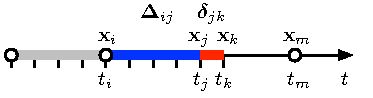
\includegraphics[width=0.6\textwidth]{figures/delta_time}
    \caption{The pre-integrated delta $\D_{ij}$ contains all motion from the last KF at time $i$, up to time $j$. 
    The current delta $\D_k$ contains the motion from times $j$ to $k$, computed from the last IMU measurement at time $k$.}
    \label{fig:delta_time}
\end{figure}

We perform pre-integration incrementally as follows. 
First, $\ol\D_{ii}$ is initialized to the null motion via the identity of the group, $\D_{\cE}$. 
Its covariance $\Cov_\Delta^{ii}$ and the Jacobian $\mjac{\D_i}{\bfb_i}$ are set to zero. 
At each reception of sensor data $\tilde\bfz_k$ at $t_k$, we integrate during $\dt$ to obtain the delta corresponding to a single data sample
%
\begin{equation}
    \bm\delta_k = f(\tilde\bfz_k, \ol\bfb_i, \dt)~, 
    \label{eq:data2delta}
\end{equation}
%
using the bias $\ol\bfb_i$ available in KF $i$. 
In major cases, this function is split into the stages of data calibration $c()$, producing a vector in the Lie algebra, and retraction $\Exp()$, retracting it onto the manifold,
%
\begin{align}
    \bftau_k &= c(\tilde\bfz_k, \ol\bfb_i) \dt \in \Reals^{dim(\cM)}\\
    \bm\delta_k &= \Exp(\bftau_k) \in \cM,
\end{align}
%
where the former, $c()$, depends on the sensor model, and the second, $\Exp()$, on the deltas Lie group.
This single delta is integrated onto the delta pre-integrated so far using the delta composition law
%
\begin{equation}
    \ol\D_{ik} = \ol\D_{ij} \circ \bm\delta_k 
    \label{eq:deltaPlusDelta}
\end{equation}
%
as can be seen in figure \figRef{fig:delta_time}.
%with Jacobians $\mjac{\ol\D_{ik}}{\ol\D_{ij}}$ and $\mjac{\ol\D_{ik}}{\bm\delta_k}$. 
The pre-integrated delta covariance, as well as the Jacobian of the pre-integrated delta with respect to biases, are also pre-integrated using the chain rule and standard covariance propagation,
%
\begin{align}
    \Cov_\Delta^{ik} &= \mjac{\D_{ik}}{\D_{ij}}\Cov_\Delta^{ij}\mjac{\D_{ik}}{\D_{ij}}\tr 
    + \mjac{\D_{ik}}{\bm\delta_k}\mjac{\bm\delta_k}{\bfz_k}\Cov_\bfz\mjac{\bm\delta_k}{\bfz_k}\tr\mjac{\D_{ik}}{\bm\delta_k}\tr
    \\
    \mjac{\D_{ik}}{\bfb_i} &= \mjac{\D_{ik}}{\D_{ij}}\mjac{\D_{ij}}{\bfb_i} 
    + \mjac{\D_{ik}}{\bm\delta_k}\mjac{\bm\delta_k}{\bfb_i} ,
\end{align}
%
where $\mjac{\bm\delta_k}{\bfb_i}$, $\mjac{\bm\delta_k}{\bfz_k}$ are the Jacobians of \eqRef{eq:data2delta} and $\mjac{\D_{ik}}{\D_{ij}}$, $\mjac{\D_{ik}}{\bm\delta_k}$ the Jacobians of \eqRef{eq:deltaPlusDelta}, computed according to Lie theory \cite{sola2018micro}, to which we give a brief introduction in \secRef{sec:lie_groups}.



\subsection{Residual definition}
\label{sec:preint_residual}

The successive $\ol\D_{ik}$, $\mjac{\D_{ik}}{\bfb_i}$, and $\Cov_\Delta^{ik}$ are kept in a buffers initialized at $t_i$. When a new \keyframe\ is added to the problem at time $k=m$,
a factor is created to which we pass $\ol\D_{im}$, $\ol\bfb_i$,  $\mjac{\D_{im}}{\bfb_i}$, and $\Cov_\Delta^{im}$, with which the residual can be defined:
%
% The pre-integrated $\ol\D_{im}$ is used at the end of the pre-integration to define the residual:
%
\begin{align}
    \bfe_{im}(\bfx^i, \bfx^m, \bias^i) = (\ol\D_{im} \oplus \mjac{\D_{im}}{\bfb_i}(\bfb_i-\ol\bfb_i) ) \ominus \hat\D_{im}
    \label{eq:preint_residual}
\end{align}
%
with associated covariance $\Cov_\Delta^{im}$.
Here, $\bfb_i$ is the current  value of the sensor's calibration parameters,  $\hat\D_{im}=\bfx^m\boxminus\bfx^i$ is the expected delta between KFs, and $\{\op,\om\}$ are the 
 plus and minus operators described in section \secRef{sec:manifold_structure}. 
% That is, $\{\op,\om\}$ are $\{+,-\}$ for vectors, and for rotations we have $\bfR\op\bm\theta\te\bfR\Exp(\bm\theta)$ and $\bfR_2\om\bfR_1\te\Log(\bfR_1\tr\bfR_2)$. 
% The residual clearly depends on the KF states $\bfx^i,\bfx^m$ and the bias $\bfb_i$. It has an associated covariance  $\Cov_\Delta^{im}$.

In cases where the calibration parameters are subject to drift, as it is the case for IMU biases, the calibration drift is modelled as the integration of a random walk. This drift is included as a factor in the factor graph by defining a residual error
%
\begin{equation}
    \bfe^{\bias}_{im}(\bias^i, \bias^m) = \bias^m - \bias^i
\end{equation}
%
with associated covariance matrix
%
\begin{equation}
    \Cov_{\bias,im} = \bfW^c_{\bias} \Dt_{im}
\end{equation}


%
%
%
%
\section{IMU pre-integration on Lie groups}
In \cite{fourmy2019absolute}, we showed that an alternative formulation of IMU preintegration on Lie groups was possible.
We introduce a new matrix Lie group representation of the IMU deltas. The complete IMU pre-integration theory,
including the computation of the residual, is based on this new Lie structure. The theoretical material for the Lie
development in this section can be found in the report \cite{sola2018micro}.

\subsection{IMU pre-integraton on composite Lie group}
\label{sec:imu_preint_composite}

Let us come back to the IMU pre-integration problem, as stated by Forster \cite{lupton-09, forster2015imu}, defined in \secRef{sec:imu_preint_motivation}, and show that we can rewrite the algorithm in terms of the generalized pre-integration described in \secRef{sec:general-preint}.

The states involved in this integration are the base states $\bfx = [\posi{}{}, \bfv, \Rot{}{}]$ with deltas $\D=[\Dp,\Dv,\DR] \in \cM_{\D}$. 
The IMU produces biased and noisy measurements $\tilde\bfz = [\tilde\bfa, \tilde{\bfomega}]$ of the base proper acceleration and angular velocity, 
with bias $\bfb = [\bias_{a}, \bias_{\omega}]$ and noise $\noise = [\noise_{a}, \noise_{\omega}]$. 

\subsubsection{Definition of the delta operations}

The group composition law $\D^{ik}=\D^{ij}\circ\bm\delta^k$ in \eqRef{eq:deltaPlusDelta} is defined as
%
\begin{equation} 
    \label{equ:composition_delta}
    \D \circ \D
    =
    \begin{bmatrix}
        \Dp^{ij} + \Dv^{ij}\dt + \DR^{ij}\dpp^{k} \\
        \Dv^{ij} + \DR^{ij}\dv^{k} \\
        \DR^{ij}\dR^{k} 
    \end{bmatrix}
\end{equation}
%
with a group identity element composed of the identity element of its Lie groups:
%
\begin{equation}
    \D_{\cE} = [\bf0_3, \bf0_3, \bfI_3],
\end{equation}
%
its the resulting inverse being
%
\begin{equation}
\label{equ:inverse_delta}
    \D^{-1} =     \begin{bmatrix}
    - \DR\tr(\Dp + \Dv \dt) \\
    - \DR\tr \Dv \\
      \DR\tr
    \end{bmatrix}
\end{equation}
%


The pre-integration method in  \cite{forster2017-TRO} can be put in the general pre-integration formalism above by defining 
$\bm\delta=f(\tilde\bfz,\bfb,\dt)$ in \eqRef{eq:data2delta} as:
%
\begin{align}
    \bm\delta^k = \begin{bmatrix}
    \delta\bfp\\\delta\bfv\\\delta\bfR
    \end{bmatrix}^k =
    \begin{bmatrix}
    \tfrac12(\tilde\bfa-\bfb_a-\noise_a)\dt^2 \\
    (\tilde\bfa-\bfb_a-\noise_a)\dt \\
    \Exp((\tilde{\bfomega}-\bfb_\omega-\noise_\omega)\dt)
    \end{bmatrix}^k
    \label{eq:delta_function}
\end{align}

Then, $\bfx_k=\bfx_i\boxplus\D_{ik}$ is \cite[eq.~32]{forster2017-TRO} and $\D_{ik}=\bfx_k\boxminus\bfx_i$ is \cite[eq.~33]{forster2017-TRO}. 
Full details can be found in \cite[Section 3.4]{atchuthan-18-thesis}.

\subsubsection{Interpretation of the IMU deltas}

\begin{figure}[h]
\centering
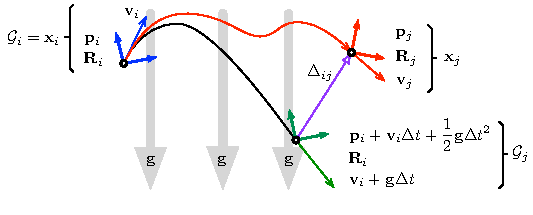
\includegraphics[width=0.8\textwidth]{figures/fff}
\caption{The free-falling, non-rotating frame $\cG_t$ follows a parabolic trajectory governed only by gravity $\bfg$ and determined by the initial conditions $\bfp_i$, $\bfv_i$ and $\bfR_i$ at time $i$ ($\cG_i=\bfx_i$, blue). The IMU delta $\D_{ij}$ between times $i$ and $j$ is defined as the state of the IMU at time $j$ ($\bfx_j$, red) expressed in the free-falling frame at time $j$ ($\cG_j$, green).}
\label{fig:fff}
\end{figure}

The IMU deltas, as introduced in \cite{lupton-09, forster2015imu} can be interpreted \cite{atchuthan-18-thesis} as the motion increments, in terms of position, velocity and orientation, between the current IMU frame and another frame, that started at the IMU state at time $i$, $\bfx_i=(\bfp_i,\bfv_i,\bfR_i)$, and falls freely and without rotating at the acceleration of gravity (\figRef{fig:fff}).



\subsection{IMU pre-integration on compact Lie group}
\label{sec:imu_preint_compact}

This formulation was proposed in our published paper \cite{fourmy2019absolute}.
We propose a matrix form of the Lie group of IMU deltas as,
%
\begin{align}\label{equ:delta_Lie}
    \D &= 
    \begin{bmatrix}
    \DR & \Dv & \Dp \\
    \bf0 & 1 & \Dt \\
    \bf0 & 0 & 1
    \end{bmatrix} \in \cD \subset \bbR^{5\times 5}
    ~.
\end{align}

Group composition, identity and inverse stem from regular matrix product, identity, and inverse (with $\DR\inv=\DR\tr$).

\begin{align}
    \D\cdot\bm\delta 
    &= 
    \begin{bmatrix}
    \DR\dR & \Dv + \DR\dv & \Dp+\Dv\dt + \DR\dpp \\
    \bf0 & 1 & \Dt+\dt \\
    \bf0 & 0 & 1
    \end{bmatrix}
    ~.
    \label{eq:compact_composition}
    \\
    \D_\cE&=\begin{bmatrix}
    \bfI_3 & \bf0 & \bf0 \\
    \bf0 & 1 & 0 \\
    \bf0 & 0 & 1 
    \end{bmatrix} = \bfI_{5\times5}
    \label{equ:identity}
    \\
    \D\inv &= \begin{bmatrix}
    \DR\tr & -\DR\tr\Dv & -\DR\tr(\Dp-\Dv\Dt) \\
    \bf0 & 1 & -\Dt \\
    \bf0 & 0 & 1
    \end{bmatrix} 
    \label{equ:inverse}
\end{align}
%
Comparing against \eqsRef{equ:composition_delta}{equ:inverse_delta} we observe that this matrix Lie group behaves equivalently to Forster's IMU deltas above.


\subsubsection{Lie algebra \texorpdfstring{$\mathfrak{d}$}{d} and exponential map}

The compact Lie group defines a different Lie algebra parametrization and therefore a different exponential map.
The Lie algebra elements $\bftau\hhat$ and their isomorphic Cartesian $\bftau$ have the forms
%
\begin{align}
    \label{equ:lie_algebra}
    \bftau\hhat &= \begin{bmatrix}
    \hatx{\bth} & \bfrho & \bfupsilon \\
    \bf0 & 0 & \Dt \\
    \bf0 & 0 & 0
    \end{bmatrix} \in \mathfrak{d}
    ,&
    \bftau &= \begin{bmatrix}
    \bfrho \\ \bfupsilon \\ \bth \\ \Dt
    \end{bmatrix}
    \te \Dt \begin{bmatrix}
    \bfv \\ \bfa \\ \bw \\ 1
    \end{bmatrix} 
    \in \bbR^{10}
    ,
\end{align}
%
with $\bfv\te\dot\Dp$, $\bfa\te\dot\Dv$ and $\hatx{\bw}\te\DR\tr\dot\DR$.
Operators $\wedge$ and $\vee$ are defined so that $\bftau\hhat=(\bftau)\hhat$ and $\bftau=(\bftau\hhat)\vvee$.

The exponential map transfers tangent elements to the group; the logarithmic map is its inverse,
%
\begin{align}
    \D &= \Exp(\bftau) \te \exp(\bftau\hhat) = \begin{bmatrix}
    \Exp(\bth) & \bfQ\bfupsilon & \bfQ\bfrho+\bfP\bfupsilon\Dt \\
    \bf0 & 1 & \Dt \\
    \bf0 & 0 & 1
    \end{bmatrix} %\in\cD 
    \label{eq:compact_exp}
    \\
    \bftau &= \Log(\D) \te \log(\D)\vvee = \begin{bmatrix}
    \bfQ\inv(\Dp-\bfP\bfQ\inv\Dv\Dt) \\
    \bfQ\inv\Dv \\
    \Log(\DR) \\
    \Dt 
    \end{bmatrix} %\in \bbR^{10}
    \label{eq:compact_log}
\end{align}
%
where $\Log()$ is obtained by identifying terms in \eqRef{equ:delta_Lie} and \eqRef{eq:compact_exp}.
Matrices $\bfP$ and $\bfQ$ are provided in the appendix's \secRef{sec:IMULieGroup}.


\subsubsection{The IMU case of \texorpdfstring{$\bfv=0$}{bfv=0}}
\label{sec:IMU_case}

We showed that IMU deltas could be interpreted as the motion relative to the free-falling frame (\figRef{fig:fff}), which has initial velocity $\bfv_i$, and the same physical analogy applies to the compact Lie group.
Thus the tangent velocity $\bfv=\dot\Dp$  is zero at the start of the integration step. 
%
Since the exponential $\Exp(\bm\nu\Dt)$ assumes a constant tangent vector $\bm\nu=(\bfv,\bfa,\bw,1)$ during the interval $\Dt$, we have that $\bfv=0$ during the full step. 
%
This gives immediately
%
\begin{equation}
    % \D &= 
    \Exp\left(\begin{bmatrix}
    \bf0 \\ \bfa \\ \bw \\ 1
    % \hatx{\bw} & \bfa & \bf0 \\
    % \bf0 & 0 & 1 \\
    % \bf0 & 0 & 0 
    \end{bmatrix}\Dt\right) 
    = \begin{bmatrix}
    \Exp(\bw\Dt) & ~\bfQ\bfa\Dt~ & \bfP\bfa\Dt^2 \\
    \bf0 & 1 & \Dt \\
    \bf0 & 0 & 1
    \end{bmatrix}
    ~,
    \label{eq:exp_compact_imu}
\end{equation}
%
which we will use to integrate IMU data.


\subsubsection{Jacobians, uncertainty}
\label{sec:uncertainty}

For general functions $f:\cM\to\cN;y=f(x)$, we propagate uncertainty normally via the Jacobians 
$\mjac{y}{x}\te\dpar{y}{x}$, \ie, $\Cov_y=\mjac{y}{x}\,\Cov_x\,\mjac{y}{x}\tr$. 
These Jacobians map the tangent spaces of the manifolds $\cM,\cN$ at $x$ and $y$, and in case of vector spaces they resort to the classical Jacobian.
They also satisfy the chain rule, which we use extensively in our developments.
Ample reference and justification of this approach can be found in \cite{sola2018micro}.

A comment is however necessary for the present IMU case.
It relates to the uncertainty of the last component of the tangent space \eqRef{equ:lie_algebra}, which is the time $\Dt$. This component has no uncertainty by definition. 
Having it in the covariances would imply singularity and result in the risk of a number of well-known numerical issues. 
We therefore systematically marginalize this time component out of the covariances, simply by removing the last row and column. 






%
%
%
\subsubsection{Pre-integration pipeline}

Here we recall the general pre-integration pipeline in the case of compact Lie group, pointing at the minor differences with composite Lie group case.
The following pipeline of operations is performed to recursively pre-integrate IMU data into a unique measurement.

At the reception of each IMU measurement $\bfz_k=(\bfa,\bw)_k$, start by correcting it with available  bias estimates $\ol\bfb_i=(\bfa_b,\bw_b)_i$, 
to produce the tangent vector $\bftau=\bm\nu\dt$. For this, set the velocity part of $\bm\nu$ to zero as the IMU is by definition at zero speed \wrt 
the moving frame, as in \eqRef{eq:exp_compact_imu}. Obtain at the same time the respective Jacobians,
%
\begin{align}
    \bftau_k &= 
    \begin{bsmallmatrix}
    \bf0 \\ \bfa-\bfa_b \\ \bw-\bw_b \\ 1
    \end{bsmallmatrix}\dt, 
    &
    \mjac{\bftau}{\bfz} &= 
    \begin{bsmallmatrix}
    \bf0 & \bf0 \\
    \bfI & \bf0 \\
    \bf0 & \bfI \\
    0 & 0
    \end{bsmallmatrix}\dt,
    &
    \mjac{\bftau}{\bfb} &= 
    -\begin{bsmallmatrix}
    \bf0 & \bf0 \\
    \bfI & \bf0 \\
    \bf0 & \bfI \\
    0 & 0
    \end{bsmallmatrix}\dt 
    \label{eq:preint_debiasing}
\end{align}
%
Second, use the exponential map \eqRef{eq:exp_compact_imu} to obtain the current delta step $\bm\delta_{jk}$ in the group manifold, and obtain Jacobian
%
\begin{align}
    \bm\delta_{jk} &= \Exp(\bftau_{k})~,
    &
    \mjac{\bm\delta}{\bftau} &= \mjac{}{r}(\bftau_k)
    ~.
    %
    \intertext{Third, use group composition \eqRef{eq:compact_composition} to update the pre-integrated delta; obtain Jacobians}
    %
    \ol\D_{ik} &= \ol\D_{ij}\circ\bm\delta_{jk} ~,
    &
    \mjac{\D_{ik}}{\D_{ij}} &= \Ad{\bm\delta_{jk}}\inv
    ~,&
    \mjac{\D_{ik}}{\bm\delta_{jk}} = \bfI
    \label{equ:pre_composition}
    ~,
\end{align}
%
where $\Ad{\bm\delta}$ is the adjoint and $\mjac{}{r}$ is the right Jacobian ---see appendices \secRef{sec:imu_compact_adjoint}, \secRef{sec:imu_compact_right_jacobian} and technical paper \cite{sola2018micro} for reference. Fourth, propagate the delta covariance
%
\begin{align}
    \bfSigma^\Delta_{ik} &= \mjac{\D_{ik}}{\D_{ij}}\bfSigma^\Delta_{ij}\mjac{\D_{ik}}{\D_{ij}}\tr 
    + \mjac{\D_{ik}}{\bfz}\bfSigma_\bfz\mjac{\D_{ik}}{\bfz}\tr
    ~,
    %
    \intertext{with $\bfSigma_\bfz$ the covariance of the IMU measurements $\bfz$, and $\mjac{\D_{ik}}{\bfz}=\mjac{\D_{ik}}{\bm\delta}\mjac{\bm\delta}{\bftau}\mjac{\bftau}{\bfz}$ computed using the chain rule. Finally, integrate the Jacobian of the delta \wrt the biases}
    %
    \mjac{\D_{ik}}{\bfb} &= \mjac{\D_{ik}}{\D_{ij}}\mjac{\D_{ij}}{\bfb} 
    + \mjac{\D_{ik}}{\bm\delta_{jk}}\mjac{\bm\delta}{\bftau}\mjac{\bftau}{\bfb}
    ~.
\end{align}
%

Pre-integration starts after each keyframe with $\ol\D_{ii} = \bfI$, $\bfSigma^\Delta_{ii} = \bf0$ and $\mjac{\D_{ii}}{\bfb} = \bf0$, using $\ol\bfb_i = \bfb_i$ the current best estimate of the bias at time $i$.
Pre-integration is complete (\figRef{fig:delta_time}) when $k=m$, which yields $\ol\D_{im}$, $\bfSigma^\Delta_{im}$ and $\mjac{\D_{im}}{\bfb}$.


\subsubsection{Factor residual}
Computation of the residual in the case of the Lie Delta group formulation follows the steps defined in \secRef{sec:general-preint}.
% However, since the Delta is directly defined as a Lie group, the formulation is actually simplified because  ... 
Use the pre-integrated Jacobian $\mjac{\D_{im}}{\bfb}$ to correct the pre-integrated delta $\ol\D_{im}$ to account for the new bias estimate $\bfb_i\neq\ol\bfb_i$,

\begin{align}
    \D_{im}(\bfb_i) &= \ol\D_{im}\cdot\Exp(\mjac{\D_{im}}{\bfb}(\bfb_i-\ol\bfb_i)) 
    ~.
\end{align}

Use \eqRef{equ:delta} as $\boxminus$ to compute the expected delta from  $\bfx_i$ to $\bfx_m$,
%
\begin{align}
    \widehat\D_{im}(\bfx_i,\bfx_m) &= \bfx_m \boxminus \bfx_i 
    ~.
\end{align}

Compute the residual in the  tangent of $\cD$ at $\D_{im}$,
%
\begin{align}
    \bfe^\D_{im}(\bfx_i,\bfx_m,\bfb_i) 
    &=\widehat\D_{im}(\bfx_i,\bfx_m) \ominus \D_{im}(\bfb_i) \\
    &=\Log(\D_{im}(\bfb_i)\inv \cdot \widehat\D_{im}(\bfx_i,\bfx_m)) \in \bbR^9
~,
\end{align}
%
and drop the $\Dt$ part from the residual after the $\Log()$ ---see comment in \secRef{sec:uncertainty}.
In this last equation, the minus operator $\ominus$ is simply the traditional Lie group "minus" operator defined in \cite{sola2018micro} and specialized for this particular group.


\subsection{About the choice of the proper Lie group}

\subsubsection{Our IMU Lie group versus Forster's method}

Mathematically, and disregarding methodology, the main difference between our method (\secRef{sec:imu_preint_composite}) and Forster's \cite{forster2017-TRO} (\secRef{sec:imu_preint_compact}) is to be found in the exponential map. 
To see it, let us consider small rotation increments $\bth=\bw\dt$ captured at each single IMU sample. 
In such cases, the matrices $\bfP,\bfQ$ appearing in the exponential map \eqRef{eq:compact_exp} and detailed in \eqRef{equ:RQP} can be approximated by $\bfP\approx\tfrac12\bfI$ and $\bfQ\approx\bfI$.
The exponential becomes,
%
\begin{align}
    \Exp\left(\begin{bmatrix}
    \bf0 \\ \bfa \\ \bw \\ 1
    \end{bmatrix}\dt\right) \approx \begin{bmatrix}
    \Exp(\bw\dt) & \bfa\dt & \tfrac12\bfa\dt^2 \\
    \bf0 & 1 & \dt \\
    \bf0 & 0 & 1
    \end{bmatrix}
~,
\end{align}
%
where we find the terms $\bfa\dt$ and $\tfrac12\bfa\dt^2$, which should sound familiar from Forster's method. 
In effect, with this approximation, if we now compact all the steps \eqsRef{eq:preint_debiasing}{equ:pre_composition} of our integration into a cumulative expression,
%
\begin{align}
    \D_{ik} = \prod_{j=i+1}^k \Exp\left(\begin{bmatrix}
    \bf0 \\ (\bfa_j-\bfa_{bi}) \\ (\bw_j-\bw_{bi}) \\ 1
    \end{bmatrix}\dt\right)
~,
\end{align}
%
it is possible (although tedious) to show that both Forster's and our method are exactly equivalent when $\bw\dt\to0$.
% , which is usually a valid hypothesis.
% These differences should not constitute an argument against Forster, since in practice we typically have extremely small steps $\bw\dt$ and the approximation holds very well.

\subsubsection{Further discussion regarding Lie group choice}

Regarding "compact group" designs, there is still another proposal, the $\SE_2(3)$ group proposed by \cite{barrau2020mathematical, brossard2021associating}, 
which can be used for IMU pre-integration. This proposal differs from ours in the following aspects:

\begin{itemize}
    \item The $\SE_2(3)$ group does not contain the time and therefore the composition law does not account for the whole integration. Some extra algebra needs to be added.
    \item The $\SE_2(3)$ group is easier to manipulate since the closed forms for the exponential map, the adjoint and the right-jacobian are easier to obtain.
    \item Our group better separates between the delta states and the velocity of these states which depend only on the IMU data.
\end{itemize}

Therefore, it is apparent that depending on the structure of the defined Lie group, we can have different designs:
\begin{itemize}
    \item Forster \cite{forster2015imu}: Composite Lie group
    \item Barrau \cite{barrau2020mathematical}: $\SE_2(3)$ compact Lie group without time
    \item Fourmy \cite{fourmy2019absolute}: Compact IMU group with time
\end{itemize}

In the context of filtering, using a compact group formulation of the robot state has been proven to improve greatly the basin of convergence of the so-called
Invariant Kalman Filter \cite{barrau2018invariant, hartley2020contact} by avoiding the need to compute jacobians around the current estimates (which is done
with the standard EKF), which may lead to an inconsistent estimate if the filter is initialized far from the optimal. 
However, this issue is not so present with factor graph optimization since we repeatedly linearize around the new estimate.
Nevertheless, it seems that compact Lie groups may provide slightly better performances than composite Lie groups \cite{brossard2021associating}, thanks 
to a more precise linearization \wrt\ the IMU biases and a covariance propagation that better represents the geometry of the problem.

However one may ask whether these more elegant mathematical formulations and slight improvements are worth the effort. Compact designs may be seen as going against
our modularity philosophy since for each new motion sensor, we need to find a new appropriate Lie group instead of being able to reuse the machinery developed
for composite groups, which is vastly simpler.

\section{Related works}


Pre-integration principles were first proposed by Lupton \cite{lupton-09} to be applied to a smoothing based visual inertial estimator. His work was motivated partly 
by the fact that previous systems required a precise initialization of position, orientation and velocity (using a specialized routine) to begin to integrate IMU measurements. 
With this new formulation, Lupton noted that pre-integration of IMU measurements permitted to use measurements immediately and delay initial orientation about the gravity
vector in particular. 
This seminal work was quickly adopted by other authors using smoothing filters \cite{carlone2014eliminating}. As pioneering as this work was, it was however 
limited by the use of Euler angles whose problematic geometric properties are notorious. Indelman \cite{Indelman-2013-7768} first proposed to use the exponential of the 
matrix rotation group instead of Euler integration and to relax the assumptions of a non-rotating and flat earth of Lupton \cite{lupton-09}. Forster \cite{forster2015imu, forster2017-TRO}
proposed the same formulation using instead quaternions. Various experiments brought to light three main problem with the Euler angle formulation, that are completely absent 
from the quaternion "on-manifold" formulation. Firstly, first order integration of angular velocities using Euler angles is approximate, which leads to accumulated errors 
for high angular velocities or sampling rate.  Secondly, the log-likelihood of the angular displacement is not invariant under the action of rigid body transformations, 
\eg the choice of the world frame influence the results of the estimation. Finally, the well known gimbal lock singularity of Euler angles has a consequence 
on the covariance IMU noise covariance propagation, which is severely degraded when the robot trajectory comes close to the singularity. 
\cite{shen2015tightly}, later improved in \cite{qin2018vins} proposed to use a more precise numerical integration procedure than the default forward Euler used by Forster. 
Eckenhoff \cite{eckenhoff2019closed} derived closed form solutions of the preintegration equations using various piecewise constant models.

Barrau \cite{barrau2020mathematical} described a coupled matrix Lie group for the propagation of preintegration errors taking into account the earth rotation for aerospace
inertial navigation system in view. This work was later extended \cite{brossard2021associating} and showed that the linearized bias update is slightly more precise than 
the work of Forster \cite{forster2017-TRO}. Le Gentil \cite{le2020gaussian} used a different trajectory parametrization framework by formulating the preintegration algorithm 
in the context of Gaussian Process smoothing. Self calibration of IMU/Camera time offsets was also developped \cite{yang2020analytic}. 
\cite{luo2021unified} derived a comprehensive collection of motion models depending on the various possible choices of reference frames and motion conditions. 

As we saw the preintegration theory began in the context of visual-inertial odometry. It was however adapted to other high rate sensors such wheel odometry \cite{quan2019tightly}, 
possibly including self-calibration \cite{deray-19-selfcalib}. In his thesis, Atchuthan (\cite{atchuthan-18-thesis}, Section 4.3) derived the general form of the preintegration 
equations as a sensor agnostic form that is integrated in state estimation WOLF \cite{sola2021wolf}. As previously mentioned, other team applied preintegration theory in the 
context of factor graph legged robot state estimation to derive new leg odometry factors \cite{hartley2018legged, wisth2019robust, wisth2020preintegrated}.
It was also applied to integrate drone dynamics to estimate external forces disturbances \cite{nisar2019vimo}.

In \chpRef{chp:underactuade_dynamics}, we propose to pre-integrate force-torque measurements that are present in some legged-robots. We show that permits to estimate the centroidal quantities of the robot as well making the kinematic bias on center of mass measurements observable. A practical implementation is demonstrated in \ref{chp:centroidal_estimation}, which is based on our paper \cite{fourmy2021contact}


%\chapter{Centroidal dynamics}
\minitoc


\section{Centroidal kinematics}
Use of the kinematic model of the robot to obtain measurements about centroidal quantities of the robot.

We need to relate base states to centroidal quantities to ground their estimate. 
For that, we can rely on the inertial-kinematic model to compute the CoM position wrt. base frame $\posi{B}{C}(\qa) \in \Reals^3$, the CoM velocity wrt. 
base frame $\vel{B}{C}(\qa, \dqa) \in \Reals^3$, the inertial matrix $\Inertia(\qa) \in \Reals^{3\times 3}$, and  the kinematic momentum due to gesticulation 
of the robot limbs $\AM_a(\qa, \dqa) \in \Reals^{3}$. 
As stated before, the computed CoM position is considered to be affected by Gaussian noise and a slowly varying bias $\posim{B}{C} = \posi{B}{C} + \bfb_{c} + \noise_c$. 
The angular velocity from the IMU is used and its bias has to be incorporated in the factor $\angvelm{}{} = \angvel{B}{B} + \bfb_{\omega} + \noise_{\omega}$.  
In the end the equations used to derive the factor are:
%
\begin{equation}
\small
\begin{split}
\COM &= \Rot{}{} (\posim{B}{C} -  \bias_{c} - \noise_{c}) + \posi{}{}
\\
\COMd &= 
\vel{}{} + \Rot{}{}((\angvelm{}{} - \bias_{\omega} - \noise_{\omega}) \times (\posim{B}{C} -  \bias_c - \noise_c) 
\\&~~~~~~+ (\velm{B}{C} - \noise_{v}))
\\
\AM &= \Rot{}{}(\Inertia (\angvelm{}{} - \bias_{\omega} - \noise_{\omega}) + \AM_a)
\end{split}
\end{equation}

Then, the residual $\bfr^{CK} \in \Reals^9$ is simply expressed as:
%
\begin{equation}
\small
\bfr^{CK}=
\begin{bmatrix}
\posim{B}{C} - (\Rot{}{}^T(\COM - \posi{}{}) + \bias_{c})
\\
(\angvelm{}{} - \bias_{\omega}) \times (\posim{B}{C} -  \bias_{p}) + \velm{B}{C} - \Rot{}{}^T(\COMd - \vel{}{})
\\
\Inertia (\angvelm{}{} - \bias_{\omega}) + \AM_a - \Rot{}{}^T\AM
\end{bmatrix}
\label{eq:CKFactor}
\end{equation}



\section{External force pre-integration}
In this section we apply the generalized pre-integration algorithm to the problem of using measured external
forces applied on a legged robot in a smoothing estimator. We propose to integrate the underactuated that we first recall. Then 
we derive the specificities of the pre-integration of external forces of a poly-articulated system. This is the main theoretical contribution
of our paper \cite{fourmy2021contact}.


\subsection{Centroidal dynamics}
\label{sec:centroidal_dynamics}
The robot dynamics is described by the well-known:
\begin{equation}\label{eq:wbdyn}
  \bfM(\q) \vq + h(\q,\vq) = \bm\tau_q + \sum_l \bfJ_l\tr \bff_l
\end{equation}
where $\q,\vq,\dvq,\bm\tau_q$ are the position, velocity, acceleration and torques of the robot in configuration space,
$\bff_l$ are the contact forces (written as 3D forces in this paper),
$\bfM$ is the generalized inertia matrix, $h$ the sum of gravity, Coriolis and centrifugal forces, and $\bfJ_l$ the jacobians of the contact points.
Because of the underactuated nature of legged robots, the configuration is often separated into $\q=(\posi{W}{B},\Rot{W}{B},\qa)$ where $\posi{W}{B}$ 
is the position in world frame of the robot base (typically, the torso or in our case the IMU), $\Rot{W}{B}$ the rotation of the base body with respect 
to the world and $\qa$ are the joint configuration of the actuated joints. 
%We will subsequently use the notation $\prescript{X}{}{[\cdot]}_Y$ to denote vectorial quantities of frame $Y$ expressed in frame $X$. A tilde $\Tilde{[\cdot]}$ denotes a noisy measurement.

While~\eqRef{eq:wbdyn} represents the whole dynamics, a subpart of it is of particular importance for legged robots.
The centroidal dynamics is written by the two equations:
%
\begin{equation}
    m \ddot{\bfc} = m \bfg + \sum_l \bff_l \quad , \quad
\dAM = \sum_l (\posi{}{l} - \COM) \times \bff_l
\label{eq:NewtonEuler}
\end{equation}
%
where $\COM,\AM$ are the position of the Center of Mass (CoM) and Angular Momentum (AM) around the CoM (both expressed in world frame), $m$ is the robot total mass, 
and the $\posi{}{l}$ are the positions of the contact points in world frame. The centroidal dynamics is an exact part of \eqRef{eq:wbdyn} and more deeply reveals 
the underactuation: the robot can move only if applying the proper forces to the environment, as the joint torques alone cannot lead to any modification 
of CoM or AM.


The classical approach in estimation of legged robot state is to first estimate the base state, and then to reconstruct the centroidal state $(\bfc,\dot{\bfc},\AM)$ using the joint position and velocity measurements, and the robot model.
This assumes that there is no direct measurement of the centroidal state.
Consequently, we are not be able to recover the exact centroidal state if there is any bias in the robot model.

Yet, we can see from the centroidal dynamics that the force measurements are connected to the variation of the centroidal state.
As observed in~\cite{carpentier2016center}, a proper fusion of the force measurements with an estimation of the state of the base makes the centroidal state observable.


\subsection{Force pre-integration factor}

The Newton-Euler equations \eqRef{eq:NewtonEuler} relate the evolution of the CoM and AM due to gravity, external forces and torques. 
In the case of a legged robot with punctual contact feet, only forces $\forcem{}{L}$ are applied at each limb contact $L$, with no torque. 
We assume that at each  limb contact we have access to noisy local force measurements $\forcem{}{L} = \force{L}{L} + \noise_f$. 
To transform them into the body frame $b$, we compute $\Rotm{}{L} \triangleq \Rot{B}{L}(\qa)  \in SO(3)$ and $\posim{}{L} \triangleq \posi{B}{L}(\qa) \in \Reals^3 $ from the joint configuration $\qa  \in \Reals^{12}$. 
The lever arm $(\posi{}{L}-\bias_c)$ in \eqRef{eq:NewtonEuler} uses a measurement of the CoM position in base frame $ \posi{B}{C}(\qa) \in \Reals^3$. 
This measure is biased due to inaccuracies in the robot model and therefore we add a bias variable to be estimated, $\bias_c \in \Reals^3$ so that $\posim{}{C} = \posi{B}{C}(\qa) + \bias_c + \noise_c$.
Assuming constant forces during each interval $\dt$ 
the integration of \eqRef{eq:NewtonEuler} yields the discrete dynamic model for the centroidal states:
%
\begin{equation}
\begin{split}
\COM^{k} &= \COM^{k-1} + \COMd^{k-1} \dt+\frac{1}{2} \bfg \dt^2 + \frac{1}{2m} \Rot{}{}^{k-1} \sum_L \Rotm{}{L}^k (\forcem{}{L}^k - \noise_{f}) \dt^2
\\
\COMd^{k}&= \COMd^{k-1} + \bfg \dt + \frac{1}{m} \Rot{}{}^k \sum_L\Rotm{}{L}^k (\forcem{}{L}^k - \noise_{f}) \dt 
\\
\AM^{k} &= \AM^{k-1} +\Rot{}{}^k \sum_L (\posim{}{L}^k  - \posim{}{C}^k +  \bias_{c}^k + \noise_{c}) \times \Rotm{}{L}^k(\forcem{}{L}^k - \noise_{f}) \dt
\end{split}
\label{eq:COMDiscrete}
\end{equation}
%
Analogously to the IMU case, it is possible to pre-integrate force measurements to derive a factor on the states 
$\bfx_c=[\COM, \COMd, \AM, \Rot{}{}]$ using deltas $\D_c=[\D\COM, \D\COMd, \D\AM, \DR]$. 
The rotation measured by the gyroscope has to be included too for the pre-integration to work. 
In this case, the bias vector is $\bias = [\bias_c, \bias_{\omega}]$. We define measurements  $\bfz^k$ to be:
%
\begin{equation}
\bfz^k = \left[ \posim{}{C}^k, \angvelm{}{}^k, \left[\forcem{}{L}^k, \posim{}{L}^k, \Rotm{}{L}^k \right]_{L=1..4}\right]
\end{equation}

The following operators are enough to particularize the  method in \secRef{sec:general-preint} to the contact forces case.
Integrating $\bfz_k$ during $\dt$ yields $\bm\delta_k$ in \eqRef{eq:data2delta} as
%
\begin{equation}
\small
    \bm\delta^{k}(\bfz^k, \bfb^i, \dt) =
    \begin{bmatrix}
    \frac{1}{2m} \sum_l \Rotm{}{L}^k \forcem{}{L}^k \dt^2
    \\
    \frac{1}{m} \sum_l \Rotm{}{L}^k \forcem{}{L}^k \dt 
    \\
    (\sum_l \posim{}{L}^k - (\posim{}{C}^k - \bias_c^i) \times (\Rotm{}{L}^k \forcem{}{L}^k ))\dt
    \\
    \Exp((\angvelm{}{}^k - \bias_{\omega}^i)\dt)
    \end{bmatrix}
\normalsize
\end{equation}
%
and the delta composition law in \eqRef{eq:deltaPlusDelta} as
%
\begin{equation}
    \D \circ \bm\delta = 
    \begin{bmatrix}
    \D\COM + \D\COMd \dt + \DR  \delta\COM
    \\
    \D\COMd + \DR  \delta \COMd
    \\
    \D\AM + \DR  \delta \AM
    \\
    \DR\dR
    \end{bmatrix}
    ~.
    \label{eq:DeltaDTCompo}
\end{equation}
%
The expected delta $\D^{ik}=\bfx^k\boxminus\bfx^i$ between KFs $i$ and $k$ reads
%
\begin{equation}
\D^{ik} =
\begin{bmatrix}
   \D\COM^{ik} \\ \D\COMd^{ik} \\ \D\AM^{ik} \\ \DR^{ik}
\end{bmatrix}
=
\begin{bmatrix}
	{\Rot{}{}^i}\tr (\COM^k - \COM^i - \COMd^i \Dt^{ik})
	\\
	{\Rot{}{}^i}\tr (\COMd^{k} - \COMd^{i} - \bfg \Dt^{ik})
	\\
	{\Rot{}{}^i}\tr (\AM^{k} - \AM^{i})
	\\
    {\Rot{}{}^i}\tr \Rot{}{}^k
\end{bmatrix}
~.
\end{equation}
%
Finally, the propagation of the state $\bfx_i$ to $\bfx_k$ using $\D_{ik}$, which can be used to retrieve a state at any time $k$ between KFs in the trajectory, is
%
\begin{equation}
	\bfx^k = \bfx^i \boxplus \D^{ik} =
	\begin{bmatrix}
	\COM^i + \COMd^i \Dt^{ik} + \Rot{}{}^i \Delta \COM^{ik} + \frac{1}{2} \bfg \Dt^{ik,2}
	\\
	\COMd^i + \Rot{}{}^i \Delta \COMd^{ik} + \grav \Dt^{ik}
	\\
	\AM^i + \Rot{}{}^i \Delta \AM^{ik}
	\\
	\Rot{}{}^i \DR^{ik}
	\end{bmatrix}
\end{equation}
%
%
%
%



\part{Applications}
\chapter{Robotic platforms}
In this chapter, we present the robotic platforms

\section{HRP2 humanoid robot}
Short because only used as a support

\section{Solo robot}
Solo is a 12 degrees of freedom, fully open source quadruped robots developed between Max Planck institute and LAAS-CNRS as part of the Open Robot Initiative 
\cite{grimminger2020open} 

\subsection{Mechanical design}
\subsubsection{Actuators}
\subsubsection{Kinematics}

\subsection{Sensors}
\subsubsection{IMU}
\subsubsection{Encoders}
\subsubsection{Joint torque}
\subsubsection{Camera}

\subsection{Sofware architecture}
Really not developed: explain how we obtained the data, time synchronization etc.


\chapter{Visual-inertial SLAM with fiducial markers}
\label{chp:absolute_vi}
\minitoc
\bigskip

Results presented in this section are adapted from our published work \cite{fourmy2019absolute}. The opinions and perspectives reflected are the ones we had
at the time.

\section{Introduction}

In this work, we are interested in quantifying how accurately a humanoid robot can be localized in a structured 3D environment.
The seminal works on localization of legged robots were using leg odometry \cite{roston1991dead}, quickly followed by contributions fusing the kinematics 
with inertial measurements~\cite{lin2006sensor}. Naturally, odometry measurements can only lead to a drift of the localization.
Based on leg odometry, the community has extended the localization performances by improving the behavior of the inertial-kinematic 
filter~\cite{bloesch2013state,rotella2014state,flayols2017experimental}, the underlying contact 
model~\cite{bledt2018cheetah,rotella2018unsupervised}, and by augmenting the odometer with exteroceptive measurements coming from cameras 
or LIDAR \cite{stasse2006real, fallon2014drift, camurri2017multisensory}.

The difficulty in fusing inertial, kinematics, and exteroceptive measurements stems from the disparity in the properties of each data source.
Inertial and kinematic measurements come at high frequency (typically 100 Hz to 1 kHz) and are cheap to process, while images and laser scans 
are obtained at some few images per second and are expensive to process. 
On the other hand, inertial measurements are quickly deprecated while images and scans provide absolute information.
This implies a rigorous synchronization between the sensors with the risk of decreasing the performances of the inertial 
estimation when images and laser scans are not carefully merged. 

These difficulties explain that the first works to merge proprioceptive and exteroceptive sensors for legged localization 
have been with staggered approach, first fusing inertial and kinematic measurements at high frequency, and then correcting 
the localization drift with absolute localization computed the from the camera and/or the LIDAR with low bandwidth and higher 
delay~\cite{nobili2017heterogeneous,fallon2014drift}.

Very recently, several concurrent approaches have been proposed to merge all relevant data in a unique estimator.
Following the recent results in UAVs localization~\cite{forster2017-TRO,leutenegger2015keyframe}, optimal estimation 
structured by a factor graph has been shown to be a very nice framework to formulate the fusion.
In~\cite{hartley2018legged}, a graph-SLAM is proposed to fuse inertial, kinematics, and visual data.
Inertial measurements are considered using Forster's pre-integration factors~\cite{forster2017-TRO}, which is recalled in \secRef{sec:imu_preint_composite}.
Kinematics data are included using a 6D factor which is also pre-integrated, taking into account the hybrid nature 
of the contact dynamics using an event-based approach.
Visual factors are also expressed as 6D factors obtained by visual odometry. Results are reported on sequences of a few meters with motion-capture ground truth.
In~\cite{wisth2019robust}, the graph-SLAM also considers inertial measurements through Forster's pre-integration, while kinematic
 measurements are pre-treated by the robot low-level system~\cite{bloesch2017two} and integrated directly as 6D factors without further consideration.
% As this work is applied to a quadruped robot, obtaining this 6D information indeed requires complex filtering in itself. 
Finally, the visual information is included as 2D pixel reprojection factors in the image space, obtained from feature tracking (KLT \cite{baker2004lucas}).
Impressive experimental results are demonstrated with long outdoor sequences, using a ground-truth obtained from off-line LIDAR reconstruction.

The pros and cons of these two approaches come from the choice of the factors, but the similarities are possibly more important than the differences.
Both use a plain Forster pre-integration~\cite{forster2017-TRO}. 
Using either visual odometry or feature tracking, both systems cannot natively benefit from the information brought by loop closure and would fail 
to exploit known map information.
In both cases, the kinematic factor is straightforward to write as a 6D probabilistic constraint.
Finally, both works can account for the very different sensor frequencies, while providing a good estimate at the higher frequency if needed.


\begin{figure}[h]
    \centering
    \begin{subfigure}{0.384\textwidth}
        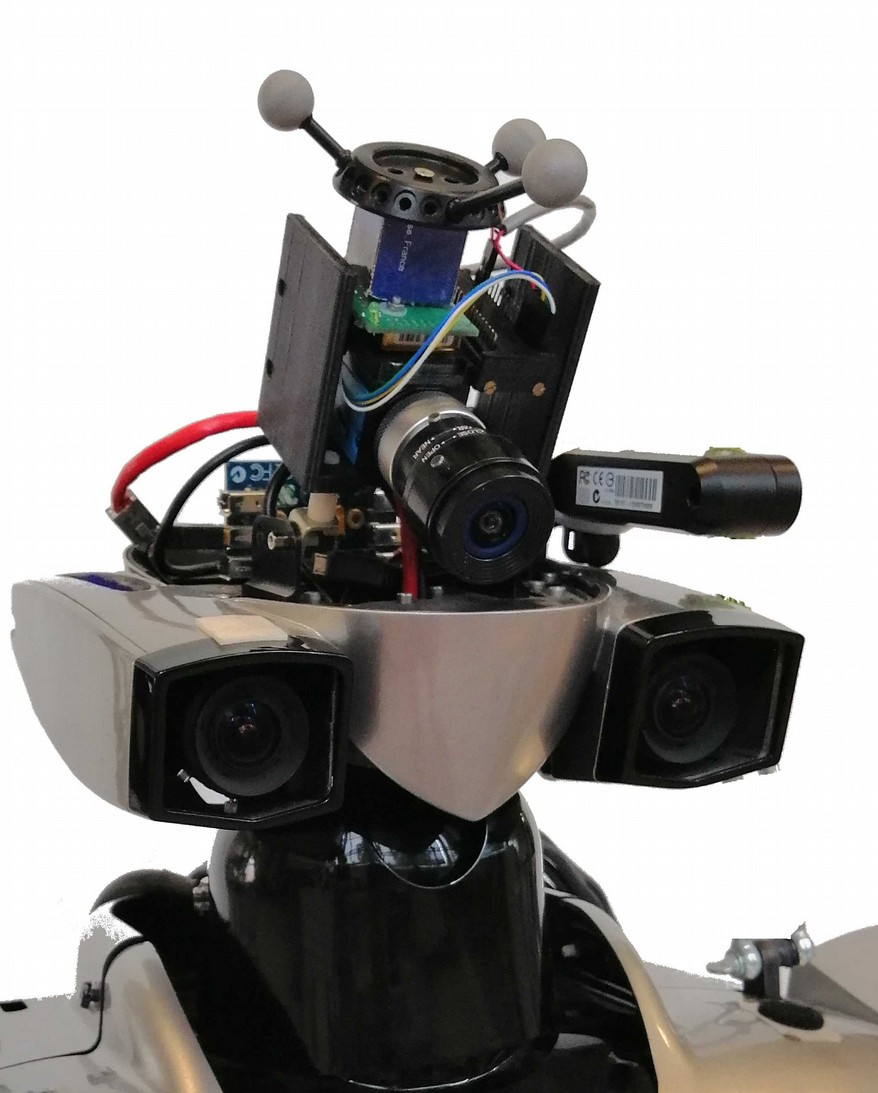
\includegraphics[width=\textwidth]{figures/absolute/HPR2_head_crop.png}
        \caption{HRP2 robot with which were conducted the experiments. The head was replaced by our visual inertial system.}
        \label{fig:HPR2_head_crop}
    \end{subfigure}
    \hfill
    \begin{subfigure}{0.546\textwidth}
        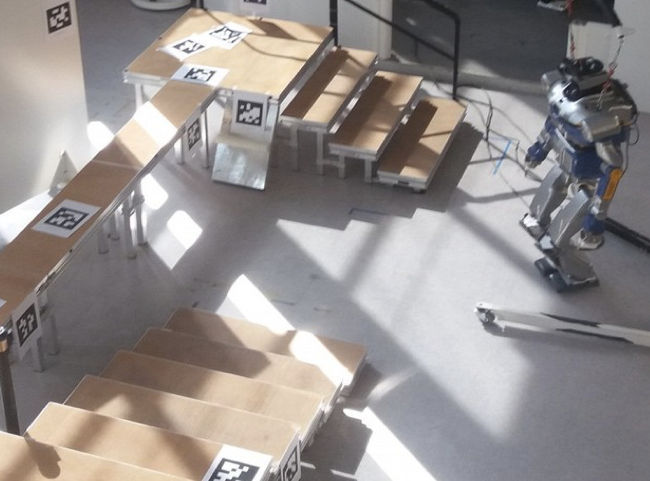
\includegraphics[width=\textwidth]{figures/absolute/bauzil.png}
        \caption{Experimental room with parkour, \HRP{2} and fiducial markers.}
    \end{subfigure}
    \label{fig:bauzil}
    \caption{Experimental setup. (\subref{fig:HPR2_head_crop}): installation of the visual inertial system. (\subref{fig:bauzil}): experimental space.}
    \label{fig:HRP2}
\end{figure}

In this work, we are looking for a solution to localize a humanoid robot indoors, with sufficient accuracy to navigate on some stairs, grasp a handrail, or 
walk on a 30-cm wide beam. 
As the robot is going to come back again and again in the same environment, we would like to benefit from loop-closure information and localization with 
respect to some known landmarks. 
While our final goal is to merge in the optimal estimator the measurements coming from all the sensors of the robot, we focus here on contributions 
validating the use of visual-inertial localization and mapping on a humanoid robot navigating indoors in a 3D environment.
For the visual factor, we rely on \apriltags \cite{wang2016iros}, while proposing a practical contribution to avoid ambiguity 
issues in the pose estimation of the tags, as described in \secRef{sec:fiducial_markers}. 
For the inertial factor, we build upon Forster pre-integration~\cite{forster2017-TRO} and propose an original,% and more rigorous theoretical formulation, 
by exhibiting a compact Lie group (described in \secRef{sec:imu_preint_compact}) that is suitable for optimal estimation. 
This formulation, although leading to very similar formulas % results -> we don't have practical results to compare 
for the inertial factors, enables a generalization to the other high-frequency factors 
that would typically arise in the humanoid contact (leg odometry based on coders, force sensors, etc).
Both inertial and visual factors are processed in a factor graph resulting in a nonlinear least-square optimization problem, solved with Ceres~\cite{ceres-solver}.

In the following section, we first formalize the inertial SLAM estimation problem that we wish to solve. Then we present experimental results on datasets obtained
with a visual-inertial system carried by a human operator and the \HRP{2} humanoid robot. 



\section{Problem statement}

\begin{figure}
    \centering
    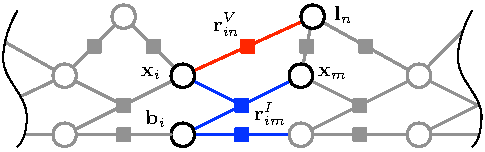
\includegraphics[scale=1.3]{figures/absolute/graph}
    \caption{A typical fraction of the factor graph, involving state blocks corresponding to keyframes $\bfx_i=(\bfp_i,\bfv_i,\bfR_i)$, biases $\bfb_i$ and landmark poses $\bfl_n$. 
    IMU factors (blue) relate consecutive keyframes and the IMU biases.
    The lower branch controls bias drift along time.
    Visual factors (red) relate landmarks with poses $(\bfp_i,\bfR_i)$.}
    \label{fig:graph}
\end{figure}

In graph-based optimization, the problem is well represented as a bipartite graph, where one type of node refers to the variables, 
and the other type called \emph{factors} represents probabilistic constraints between variables, produced by the measurements.
%
% The state $\bfx$ is modeled as a multi-variate Gaussian distribution.
In the case of landmark-based visual-inertial SLAM (see \figRef{fig:graph}), $\bfx$ includes robot poses and velocities 
$\bfx=(\bfp,\bfv,\bfR)$ and IMU biases $\bfb$, both at selected \keyframes\ along the trajectory, and landmark poses $\bfl \in \SE(3)$.
Biases are considered constant between \keyframes\.
%
In line with the recent works on the subject, we write the MAP optimization as the least-squares minimization (\figRef{fig:graph}),
%
\begin{align}\label{equ:least_squares}
    \cX^* = \argmin_\cX 
    \sum_i \norm{\bfr^I_i(\cX)}_{\Cov^I_i}^2
    +
    \sum_j \norm{\bfr^V_j(\cX)}_{\Cov^V_j}^2
    % +
    % \sum_c \norm{\bfr_c(\bfx)}_{\Sigma_c}^2
~,
\end{align}
%
with $\{\bfr^I,\Cov^I\}$ and $\{\bfr^V,\Cov^V\}$ indicating the residuals and covariances of respectively the inertial (IMU) and visual factors.
These residuals are computed differently depending on the nature of the measurements and the state blocks they relate to. 
The \apriltag\ factor is described in this thesis \chpRef{chp:object_level} and the IMU factor in \chpRef{chp:preintegration}.


\subsection{Results}

\subsection{Experimental setup}
We have gathered several datasets in the experimental arena of the humanoid robots at LAAS-CNRS, a 3D environment about $10m \times 5m$ made of flat floor, stairs of various slopes, and a 30cm wide beam.
The robot environment was augmented with about 20 fiducial ``\apriltag'' markers (of about 20 cm width).
The tags have been randomly dispatched in the environment.
They are fixed during a run but may vary significantly between two sets of data, and their locations are not calibrated ---that is, we do not have ground-truth localization of the tags.

Each dataset is composed of 3 sequences:
\begin{itemize}
    \item a sequence of RGB images captured at 33 Hz
    \item a sequence of IMU measures captured at 200 Hz
    \item a sequence of motion-capture (MoCap) at 200Hz measurements used as ground truth.
\end{itemize}


\begin{figure}[t]
    \centering
    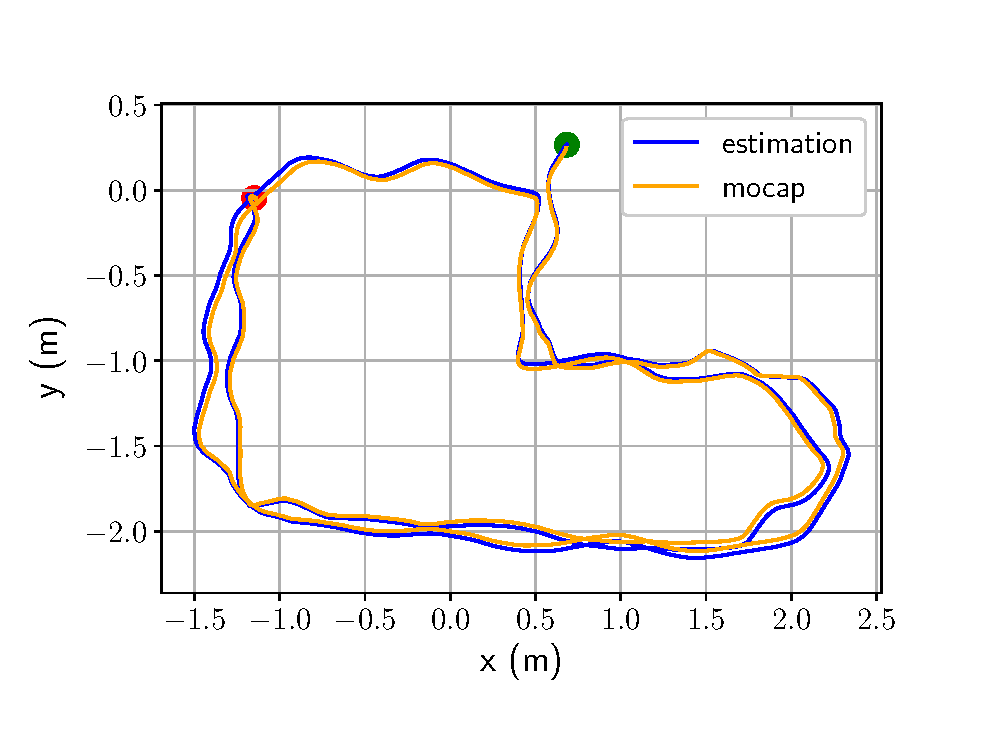
\includegraphics[scale=0.8]{figures/absolute/xy_loop_twice.eps}
    \caption{Two loops of the experimental field with camera in hand}
    \label{fig:xy_loop_twice}
\end{figure}

%
\begin{table}[t]
    \centering
    \caption{Datasets description and results}
    \begin{tabular}{c|c|c|c|c}
        Description & Duration & Length & MTE$^1$ & STE$^2$ \\
        \hline
        \hline
        Handheld loop & 59.0\,\textrm{s} & 20.6\,\textrm{m} & 29.0 & 11.3  \\
        \hline
        HRP2 turns then walks & 59.9\,\textrm{s} & 12.87\,\textrm{m} & 30.9 & 15.7 \\
        \hline
        HRP2 climbs stairs & 47.1\,\textrm{s} & 6.25\,\textrm{m} & 13.9 & 6.3 \\
        \hline
        HRP2 descends stairs & \, 19.39\textrm{s} & \, 2.62\textrm{m} & 30.4 & 11.8 \\
        \hline
        \multicolumn{5}{l}{$^1$ Mean translation error [mm]} \\
        \multicolumn{5}{l}{$^2$ Std. dev. of translation error [mm]} 
    \end{tabular}
    \label{tab:datasets}
\end{table}


The visual-inertial sensor (VIS) is comprised of a Memsic IMU running at 200 Hz and an Imagine Source camera.
IMU and camera are hardware synchronized: the image acquisition is triggered by a micro-controller (STM32) synchronized with the IMU.
We have validated that there is less than a 2 ms synchronization error by the hardware (shutter time) and that this delay is stable.
The camera and the IMU are collocated, with less than 10 cm of distance between IMU and camera focal. 
The camera-to-IMU extrinsics parameter was calibrated using the Kalibr library \cite{furgale2013unified}.
% Although our implementation of the least-squares estimator can handle sensor calibration, we have not tried to calibrate the camera-to-IMU extrinsic parameters online.
In each sequence, we have taken care that the camera is navigating in a comfortably-dense field of tags, even if it may not have always a tag in its field of view.
The motion-capture data have been obtained from a calibrated 3D marker attached to the camera and are synchronized in post-process by maximizing the velocity norm 
cross-correlation between MoCap and estimated state sequences.
% The datasets are available at \url{https://gepgitlab.laas.fr/loco-3d/wolf-data/}.
%In order to gather datasets to test our estimator, we designed a Visual Inertial System (VIS) comprised of a Memsic IMU running at 200Hz synchronized through a 
% micro-controller (STM32) with an Imagine Source camera which captures are hardware triggered. Noises parameters of the IMU were estimated using the 
% Allanvariance method described in \cite{el2007analysis}.
%We recorded several datasets in which the camera was either handheld or mounted on the head of a HRP2 humanoid robot. Rosbags for the datasets are available at 
% [url]. Ground truth is also provided thanks to a [brand name] motion capture system (mocap) recording the system pose at 200Hz.
%
\begin{figure}[t]
     \centering
     \begin{subfigure}{0.5\textwidth}
         \centering
         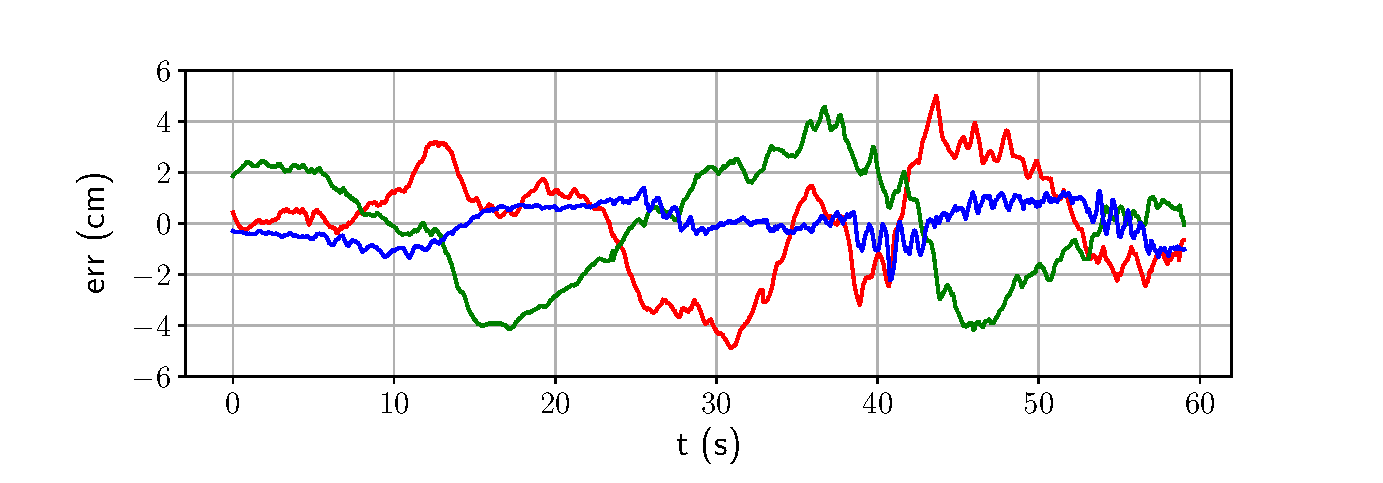
\includegraphics[width=\textwidth]{figures/absolute/terr_loop_twice.eps}
     \end{subfigure}%
     \hfill
     \begin{subfigure}{0.5\textwidth}
         \centering
         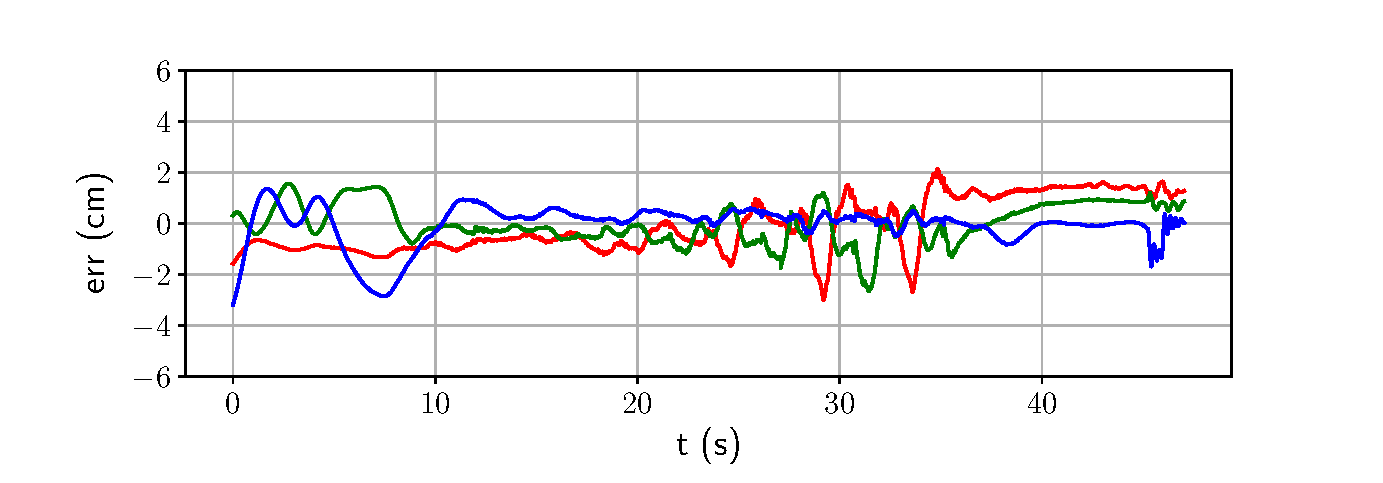
\includegraphics[width=\textwidth]{figures/absolute/terr_stairs1.eps}
     \end{subfigure}%
     \\
    \begin{subfigure}{0.5\textwidth}
         \centering
         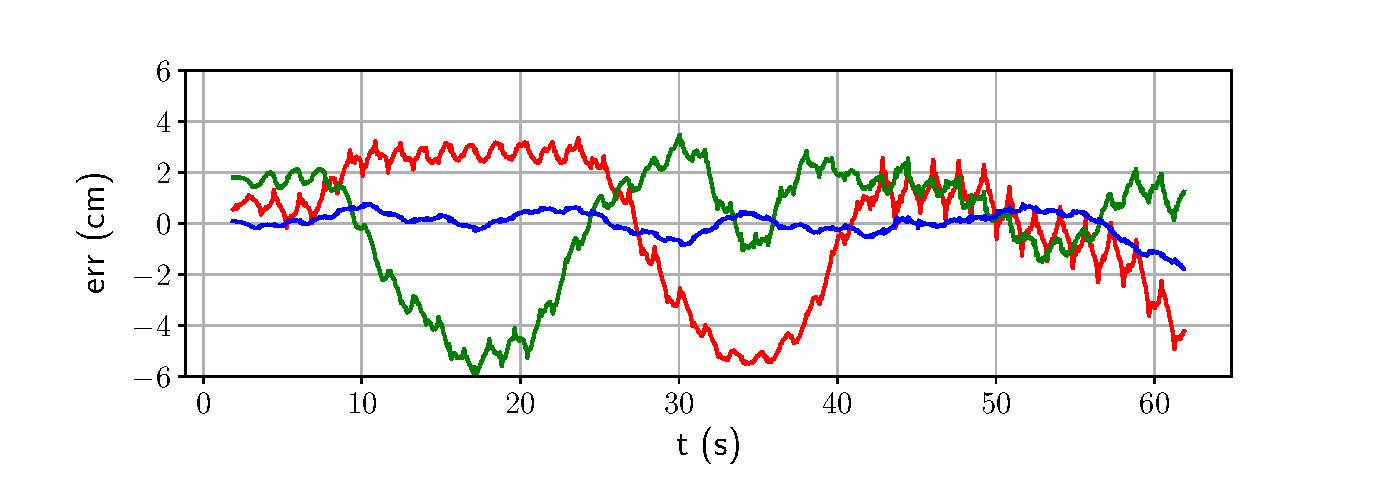
\includegraphics[width=\textwidth]{figures/absolute/terr_robot1_walking.eps}
     \end{subfigure}%
     \hfill
     \begin{subfigure}{0.5\textwidth}
         \centering
         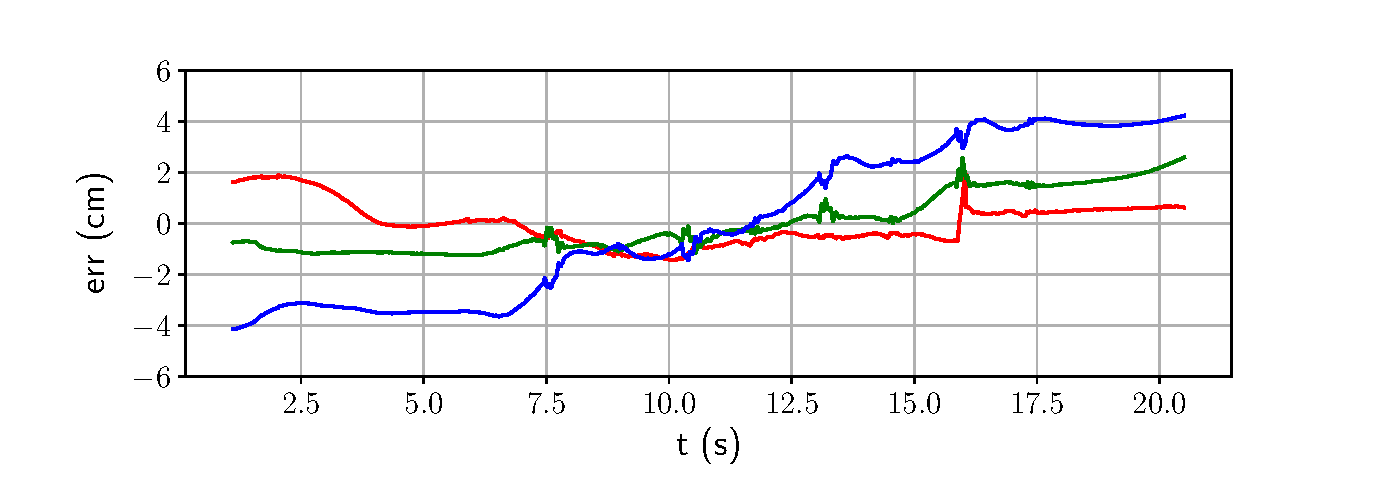
\includegraphics[width=\textwidth]{figures/absolute/terr_descending2.eps}
     \end{subfigure}%
    \caption{Translation estimation error (cm) as a function of time (s). In the clock-wise sens, starting from the 
             top-left corner, the datasets are handheld camera, stairs climbing, stairs descending and walking on flat ground. 
             RGB colors correspond to xyz axes.}
    \label{fig:results}
\end{figure}


\subsection{Localization precision}

We consider four datasets that are summarized in table \tabRef{tab:datasets}. They cover different tasks on which a consistent 
estimation of the robot movement is necessary. The first one is a relatively long sequence consisting of two loops with the VIS handheld. 
This is used to test the long-term localization of the robot, which is interesting for navigation. Secondly, we made the LAAS Gepetto team 
\HRP{2} walk and turn around on a short distance to evaluate the resilience of the filter to the vibrations of the robot. Finally, two more 
challenging datasets are recorded while the robot is climbing and descending stairs. Especially on the latter, the locomotion causes impacts 
that on one hand bring the IMU close to its dynamic range saturation, and on the other hand, provoke images with motion blur. Note that during these experiments, 
the estimator was not used for feedback control. To compare our results with the ground truth, we used methods described in \cite{zhang2018tutorial} to align 
trajectories given that 4 DoFs are unobservable in VI estimation.
For each case, \keyframes\ are created at a frequency of 6.6 Hz (every 5 images) if tags are detected in the corresponding image.

\begin{figure}[h]
    \centering
    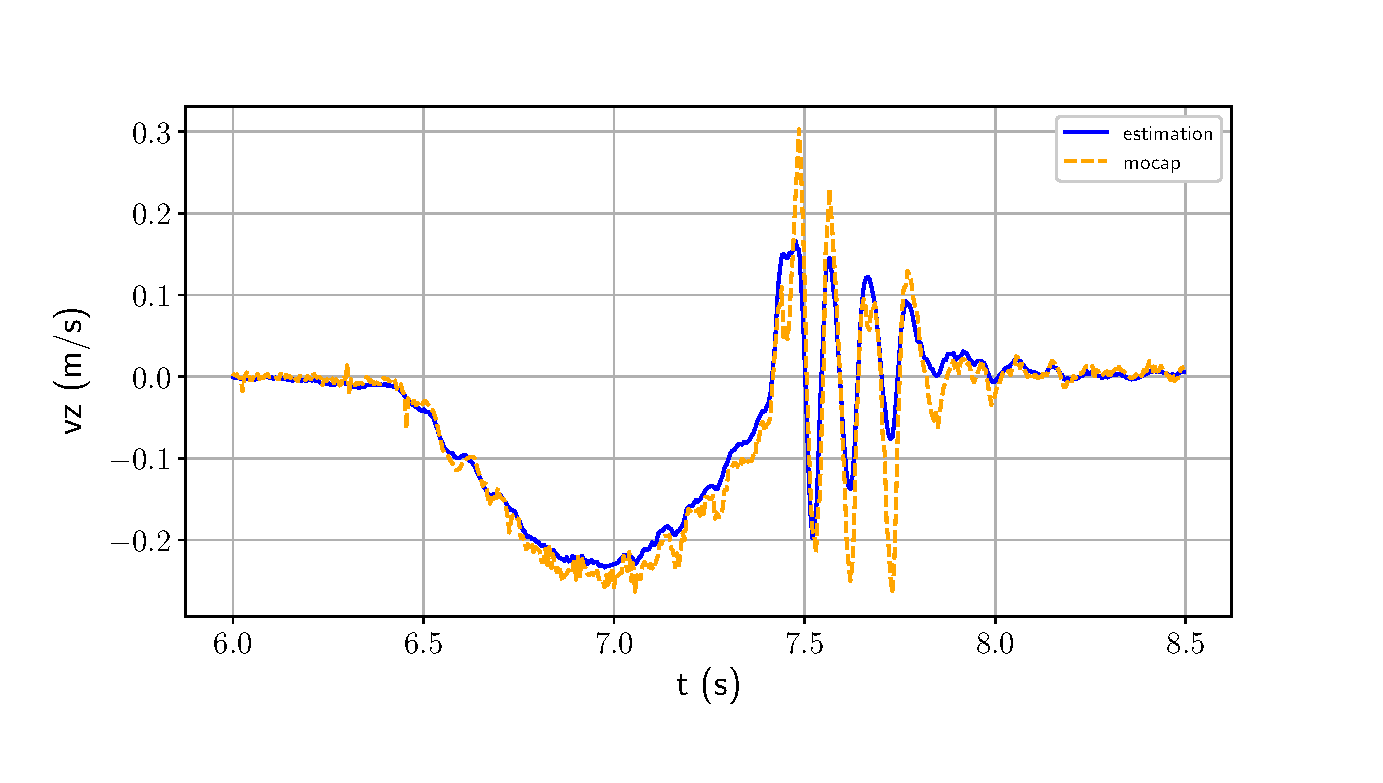
\includegraphics[width=0.8\textwidth]{figures/absolute/vz_descending_onestep.eps}
    \caption{Descending stairs (one step): the robot first lowers its center of mass and then touches the next step with results in vibrations from the impact.}
    \label{fig:vz_descending_onestep}
\end{figure}

\figRef{fig:results} presents a quantitative evaluation of the translational errors. In all cases, our estimator achieves errors consistently below a few centimeters. 
The biggest errors are obtained for the walking datasets where the two humps correspond to phases where the robot is turning on itself and sees landmarks that will not be 
seen again later in the trajectory.

A high rate estimation of a humanoid robot velocity and in particular of its center of mass is critical for balance controllers. It can be recovered from motion capture through numerical differentiation of the positions, but this results in a quite noisy time series. It is especially visible when hard impacts make the robot shake at approximately 10 Hz. 
The estimated velocity follows a familiar oscillatory damped system behavior while the mocap estimation is more erratic. 
%In this sense, our estimator seems to be more fit for feedback control than the use of the MoCap.


\subsection{Related works}
Two \apriltag\ based visual-inertial SLAM systems have been implemented in the previous years. 
In \cite{neunert2016open}, the authors rely on an EKF in which state propagation is naturally 
handled by the IMU and each marker detection is used in an update step where the reprojection error of its 4 corners provides an 8D innovation vector. 
A closer solution to ours was very recently proposed in \cite{he2019lightweight} and is also based on graph SLAM optimization benefiting from 
Forster's IMU pre-integration from GTSAM. As explained previously, the \apriltag\  factor formulation is different from ours and the algorithm is tested 
on large datasets consisting only of smooth motions.

\chapter{Centroidal estimation}
\label{chp:centroidal_estimation}
\minitoc
\bigskip


In this chapter, we propose a tightly-coupled estimator of the base and centroidal states that fuses IMU, kinematics, centroidal kinematics, 
and force-torque measurements. This work was first presented in our published paper \cite{fourmy2021contact}.

\section{Introduction}

As mentioned in the literature review, centroidal states are key to the control of legged robots. Indeed, they provide rich information about the general
behavior of the system and can be used to check for the stability of the system. The centroidal state estimation literature is rich, especially for humanoid
robots (see \secRef{sec:centroidal_est_lit}). To our knowledge, all of the centroidal estimators proposed in the literature can be classified as loosely-coupled estimators 
(following the terminology introduced in \secRef{sec:proprio_filters}): they rely on prior knowledge of a base state. For instance, Piperakis \cite{piperakis2018nonlinear} 
describes the whole pipeline: first, an inertial-kinematics EKF estimates the base state, then an EKF uses this fixed base state to obtain centroidal states. 
Since the factor graph optimization framework that we use theoretically reaches its full potential when the maximum number of cross-correlation
are considered, we did not find this solution satisfactory. Here, we rather propose a tightly-coupled estimator that jointly estimates
base and centroidal states using IMU, kinematics, and force measurements.



To the best of our knowledge, this is the first time an estimator tightly couples forces, IMU, and proprioception to estimate both base and centroidal
quantities. This estimator finds its roots in visual-inertial SLAM as described in the previous chapter,
and in the observability studies of centroidal quantities, already discussed in \secRef{sec:centroidal_dynamics}. We then skip here a discussion of related
works which has been sufficiently covered, to directly describe the underlying factor before exhibiting the experimental results.


% We present results of the application of the estimator on a dataset taken at LAAS-CNRS on the open-source robot Solo-12 \cite{grimminger2020open}:
% \textit{sinXYZ} corresponds to a trajectory where the robot moves by following a sine wave reference with the feet fixed in place. 
% This movement and another one are displayed in the companion video \url{https://peertube.laas.fr/videos/watch/16822d27-3557-4e35-9a0d-ce5b0aea4c27}.

% We use the state estimation framework WOLF developed at IRI-Barcelona, which relies on Google Ceres \cite{ceres-solver} as the graph solver. 
% The robot kinematics and dynamics computations are handled by the Pinocchio library \cite{carpentier2019pinocchio}. For all runs, \keyframes\ were created 
% at 4 Hz for a fair comparison.



\section{Problem statement}

We define here an estimator capable of observing both base states (position, orientation, velocity) and centroidal states (CoM, CoM velocity, angular momentum) from proprioception
only. We assume that the following measurements are available on the robot: IMU data, kinematics (leg odometry), centroidal kinematics, and force-torque sensors. 
Since the IMU measurements \eqRef{eq:imu_meas_model} and CoM local position from the kinematics \eqref{eq:com_kine_meas} are biased, we also need to integrate them to the estimated
variables.

Bloesch \cite{bloesch2013state} showed that the base states of legged robots and IMU biases are observable using a tightly-coupled estimator based on IMU and kinematics measurements.
On the other end, Rotella \cite{rotella2015humanoid} showed that the centroidal state of a robot and a bias on the centroidal kinematics can be obtained by fusing 
force-torque sensor measurements with centroidal kinematics, based on prior knowledge of the base states. We join the two problems into a single state estimation problem, 
represented by the factor graph of \figRef{fig:centroidal_factor_graph}.  

\begin{figure}[t]
    \centering
    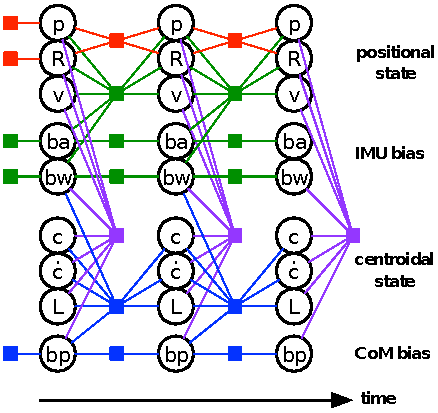
\includegraphics[width=0.6\textwidth]{figures/centroidal/centroidal_factor_graph.pdf}
    \caption{Factor graph representation of the tightly-coupled base-centroidal state estimation problem.
             Each round node corresponds to an estimated state variable. Each square corresponds to a factor, that is a measurement residual.
             The colors of the residuals are as follows. \textbf{Red}: leg odometry (\secRef{sec:leg_odometry}), \textbf{green}: IMU pre-integration and IMU bias drift 
             (\secRef{sec:preint_residual}), \textbf{purple}: centroidal kinematics (\secRef{sec:centroidal_kinematics}), \textbf{blue}: force-torque pre-integration and
             centroidal kinematics bias drift (\secRef{sec:force_torque_preint}).
             }
    \label{fig:centroidal_factor_graph}
\end{figure}

In this estimator, we have two motion sensors, IMU and force-torque, whose measurements we pre-integrate as explained in \secRef{sec:imu_preint_composite} and
\secRef{sec:force_torque_preint} respectively. Base states and centroidal states are tightly constrained by the centroidal kinematics factor, which relates almost all 
estimation variables at a given \keyframes.

\section{Experimental setup}
\label{eq:expe_setup_centroid}

This estimator is implemented in WOLF \cite{sola2021wolf}, with necessary kinematics and dynamics quantities computing
with Pinocchio software \cite{carpentier2019pinocchio}, and is experimentally validated on the Solo-12 quadruped robot. 

As is often the case with quadruped robots, Solo-12 is not equipped with three-axis force sensors at its feet. 
Yet, in order to validate the present method, it is possible to reconstruct the contact forces based on the robot dynamics 
equation \eqref{eq:wbdyn}. Knowing the robot configuration and derivatives $\q,\vq,\dvq$, and joint torques $\bm\tau$ (from motor currents), 
recovering forces from this equation results in solving an over-determined linear system. Some of these quantities are hard to obtain directly 
since they depend on the state being estimated (\eg base orientation) or on numerical differentiation ($\ddqa$). For these reasons, we pre-calculated 
these forces by benefiting from an internal filter of the 3DM-CX5-25 IMU for the base orientation, centered window differentiation of encoder speed 
measurements for the articulation acceleration $\ddqa$, and neglecting the influence of linear velocity. Fig. \figRef{fig:force_est} shows an example of 
the force reconstruction of one leg using the robot proprioceptive sensors.
%
\begin{figure}
    \centering
    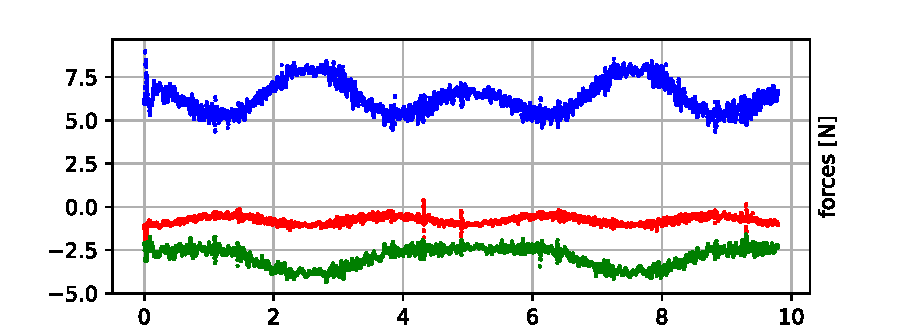
\includegraphics[width=0.9\columnwidth]{figures/centroidal/forces_solo_1leg.pdf}
    \caption{Force estimation on X-Y-Z axis (r-g-b) of one Solo-12 leg expressed in world frame using proprioceptive sensors during the \textit{sinXYZ} trajectory}
    \label{fig:force_est}
\end{figure}

This movement and another one are displayed in the video \url{https://peertube.laas.fr/videos/watch/16822d27-3557-4e35-9a0d-ce5b0aea4c27}.
The configuration trajectories were obtained using task space inverse dynamics \cite{adelprete:jnrh:2016} and applied to the robot with joint-level admittance control.


\section{Results}

\subsection{Base estimation through inertial kinematic fusion}
First, to validate the use of our kinematic factor, we include uniquely the IMU and leg-odometry factors to obtain an Inertial Kinematics estimator which 
conceptually includes the same information as estimators such as \cite{bloesch2013state}. In \figRef{fig:PosiIK4}, we compare our state estimation 
at 1 kHz with motion capture (Mo-Cap) up-sampled from 200 Hz to 1 kHz.
Velocity in the base frame is also shown in \figRef{fig:VelIK4}.

\begin{figure}[h]
    \centering
    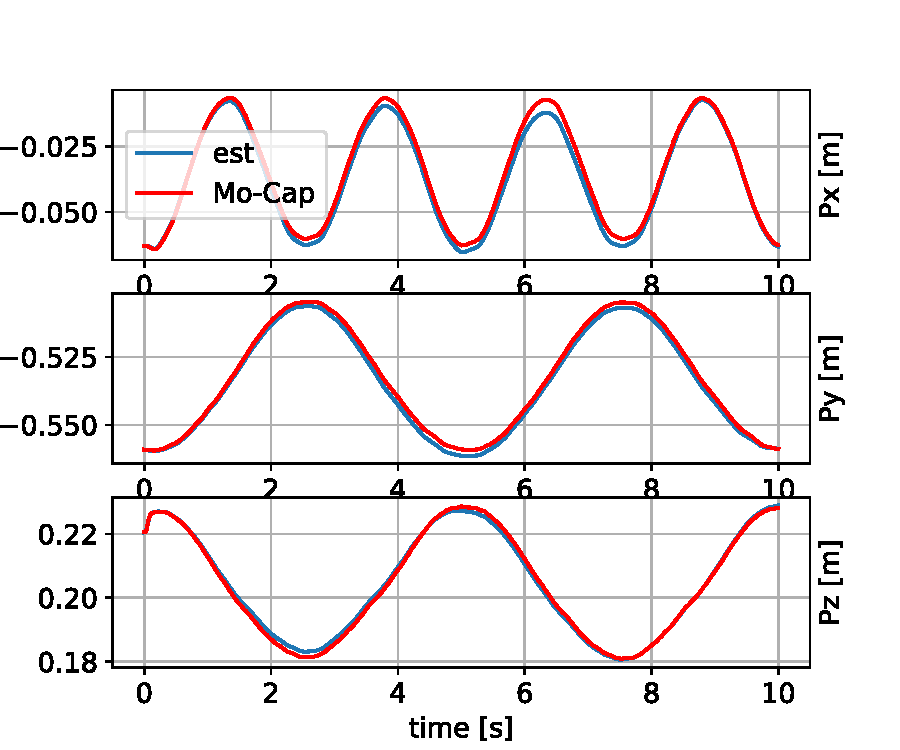
\includegraphics[width=0.6\textwidth]{figures/centroidal/base_position_IK4.pdf}
    \caption{\textit{sinXYZ} trajectory base position from the IMU+Kinematics (IK) estimator (blue) vs Mo-Cap (red)}
    \label{fig:PosiIK4}
\end{figure}

\begin{figure}[h]
    \centering
    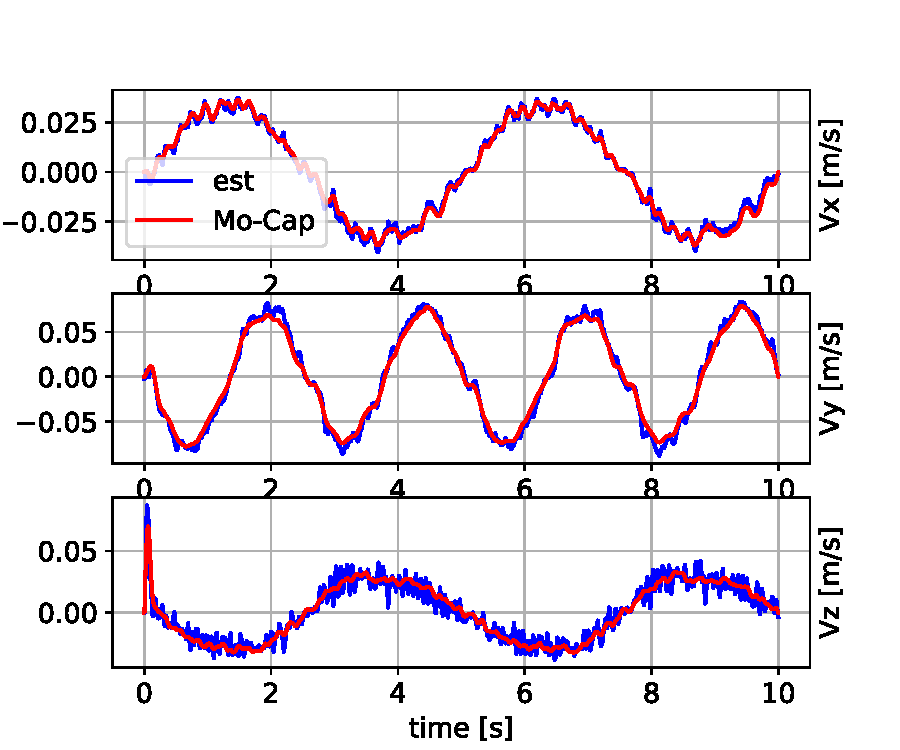
\includegraphics[width=0.6\textwidth]{figures/centroidal/base_velocity_base_frame_IK4.pdf}
    \caption{\textit{sinXYZ} trajectory base velocity in base frame from the IMU+kinematics estimator (blue) vs Mo-Cap (red)}
    \label{fig:VelIK4}
\end{figure}

Artificially removing contact factors (considering only 1, 2, or 3 feet in contact) can help us gain confidence in the use of this kinematic factor 
in situations where we rarely have all feet in contact, like for example with trotting gaits. In \figRef{fig:ErrIKn}, we can see that only considering 
1 foot in contact during the whole trajectory results in a drifting position, but as soon as 2 or more feet are in contact, the system is constrained enough 
for the drift to remain below around 5mm on all axes. 
%
\begin{figure}[h]
    \centering
    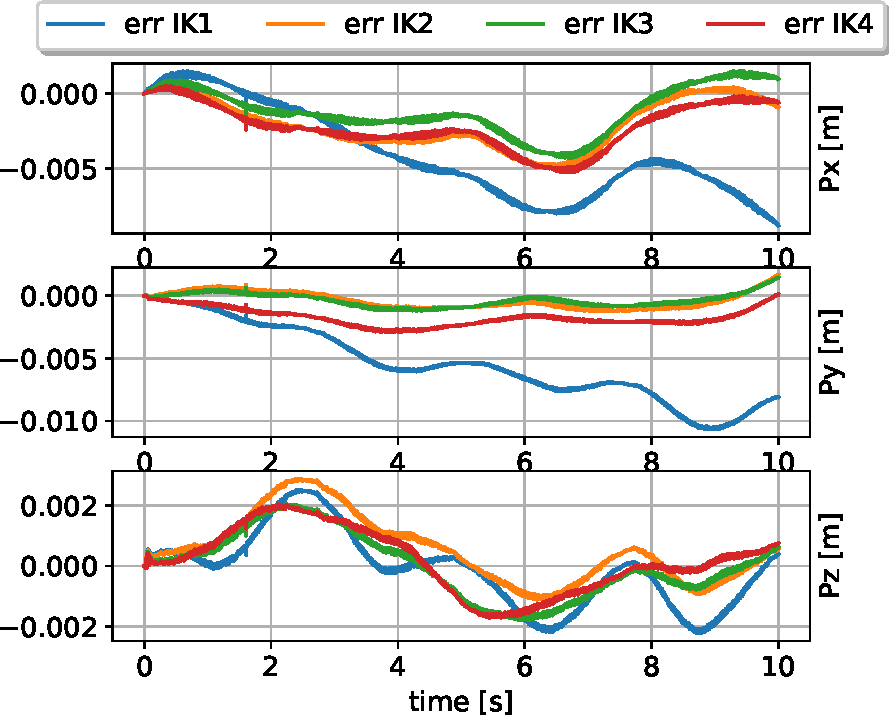
\includegraphics[width=0.6\textwidth]{figures/centroidal/base_position_err_IKn.pdf}
    \caption{\textit{sinXYZ} trajectory base position error with different numbers of feet used for the leg-odometry factors: 
    1 (blue), 2 (orange), 3 (green), 4 (red) from the IMU+kinematics estimator}
    \label{fig:ErrIKn}
\end{figure}
%

\subsection{Centroidal estimation}

Now, on the same trajectory, we deploy the full estimator with all factors described in the factor graph in \figRef{fig:centroidal_factor_graph} to jointly 
estimate the base and centroidal quantities. A ground truth on the centroidal quantities is difficult to obtain since no direct 
sensor can provide us with this information contrary to the base state. 
We can however validate our method by comparing it to a two-step procedure: first, estimate the base state with a state Kalman filter as 
implemented in \cite{bledt2018cheetah}, then compute the centroidal quantities directly from the robot kinematic model. 
The full estimator should be able to infer a bias on the $\posim{B}{C}$ measure so we artificially add a constant disturbance 
in the robot dynamic model on the lever of the base link of [0.03, 0.06, 0.04]\,cm, which then corresponds to a CoM bias of 
[-0.0197, -0.0394,  0.0263] cm. \figRef{fig:bias_est} shows that the bias estimated with our method closely matches the introduced bias. 
\figRef{fig:comparison_KF_wolf} shows a comparison between the base and CoM reconstruction with our method and with the two-step base Kalman filter 
with geometric CoM. Note that the base-CoM difference on the z-axis reflects the fact that the limbs of the robot naturally lower its CoM. 
The estimated CoM velocity closely follows the velocity of the base as shown in \figRef{fig:com_base_vel}.


\begin{figure}[h]
    \centering
    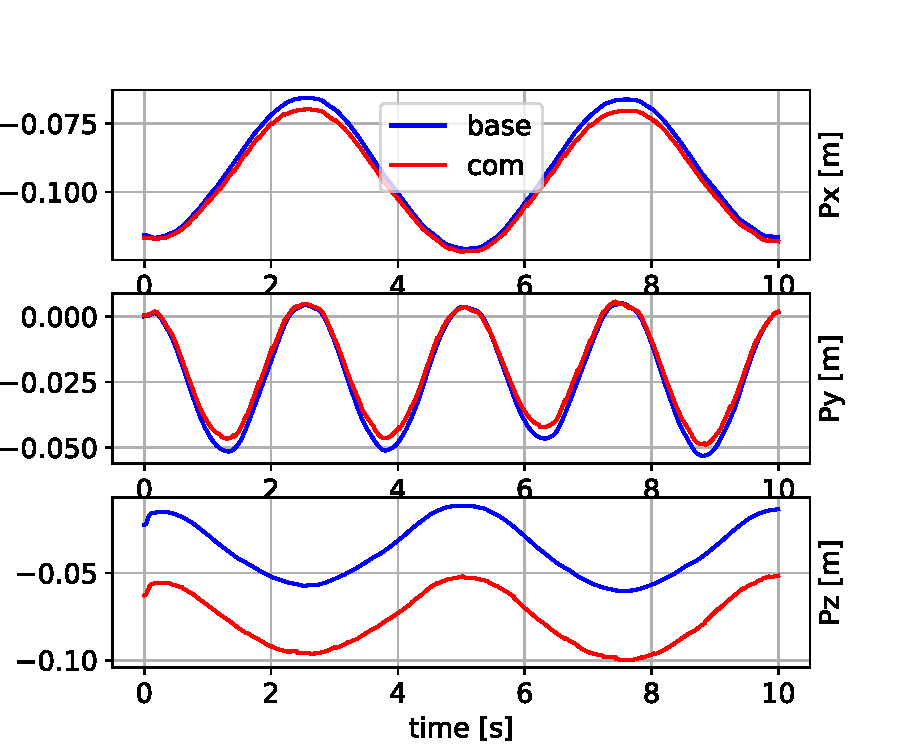
\includegraphics[width=0.6\textwidth]{figures/centroidal/com_position_povcdl_sin.pdf}
    \caption{Base position (blue) vs CoM (red) from the full estimator}
    \label{default}
\end{figure}

\begin{figure}[h]
    \centering
    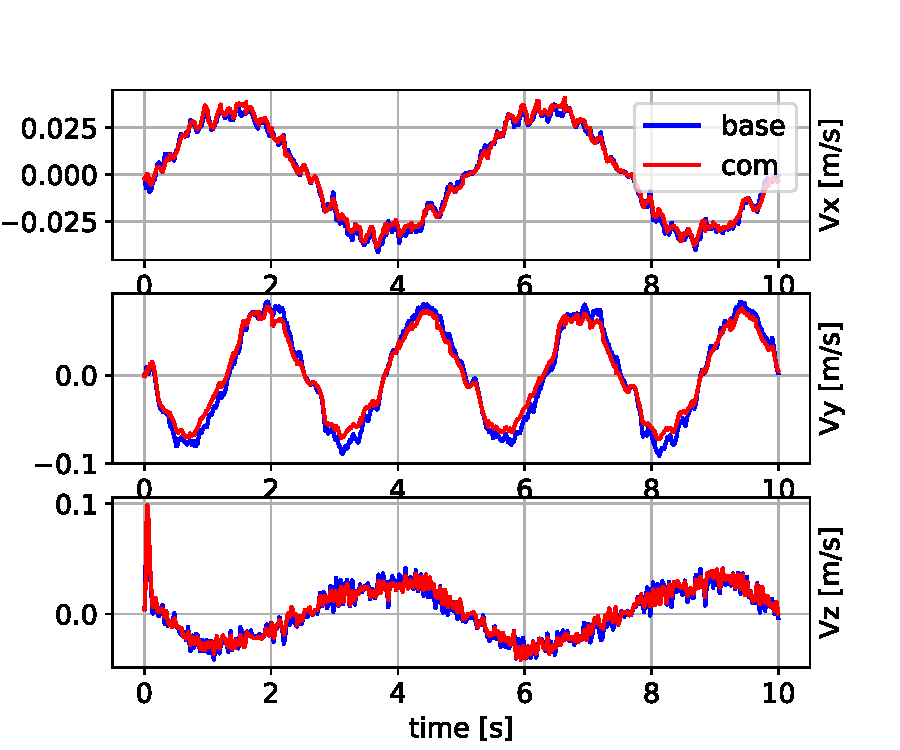
\includegraphics[width=0.6\textwidth]{figures/centroidal/com_velocity_povcdl_sin.pdf}
    \caption{Base (blue) vs CoM (red) velocities   from the full estimator}
    \label{fig:com_base_vel}
\end{figure}


\begin{figure}[h]
    \centering
    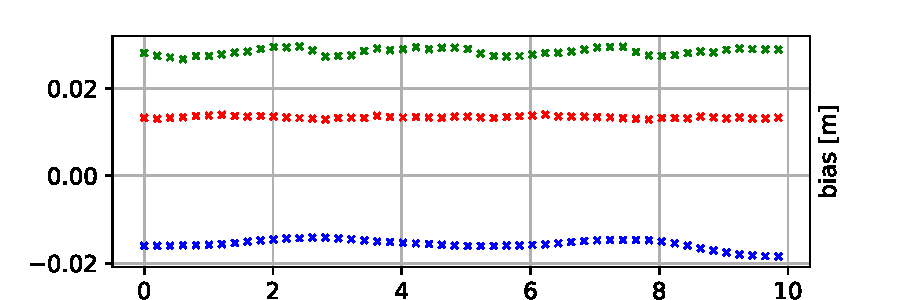
\includegraphics[width=0.6\textwidth]{figures/centroidal/com_bias_est.pdf}
    \caption{Estimation of bias on CoM measurement from the full estimator along x-y-z axis ( red-green-blue) in base frame}
    \label{fig:bias_est}
\end{figure}

\begin{figure}[t]
    \centering
    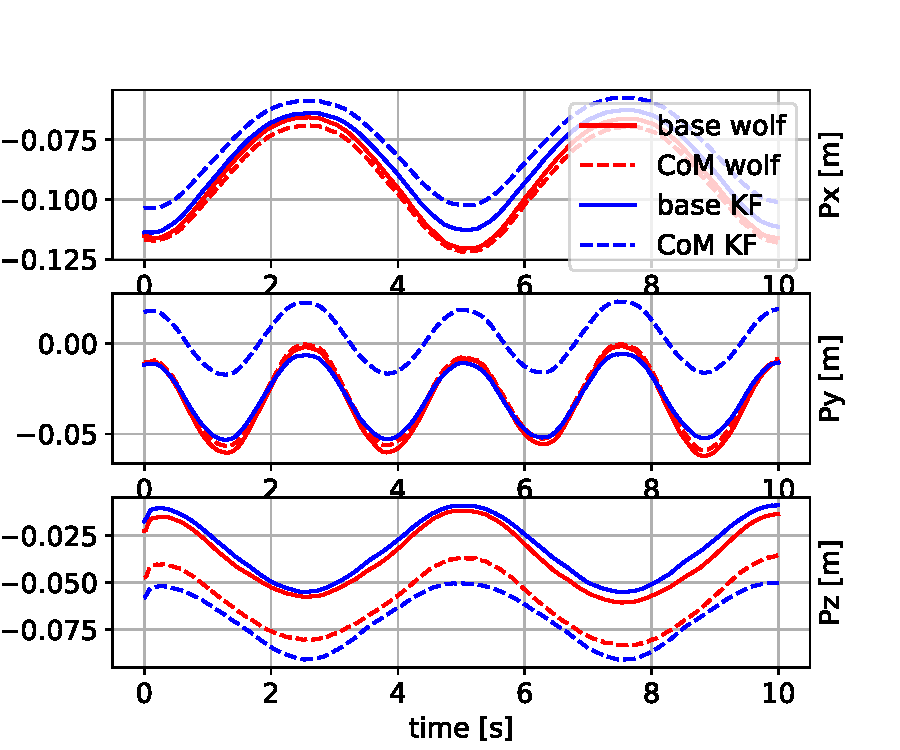
\includegraphics[width=0.6\textwidth]{figures/centroidal/base_com_position_wolf_vs_KF.pdf}
    \caption{Comparison of the estimates between decoupled the Kalman filter base estimator and geometric CoM reconstruction (blue) and 
    the tightly-coupled estimator presented in this paper (red) on the \textit{sinXYZ} trajectory with artificial base link CoM bias.}
    \label{fig:comparison_KF_wolf}
\end{figure}


\section{Discussion}

On the theoretical side, the correlation of the IMU and forces pre-integration models (due to the common gyroscope data integration) might also be investigated. 
One of the hypotheses involved in factor graph MAP estimation is the conditional independence of measurement data (see \eqRef{eq:factorized_likelihood} in \secRef{sec:MAP} for more details).
Using the same measurements for both factors violates this assumption. Our model is not an exception in MAP estimation: for example, \cite{wisth2019robust} uses 
integrates the velocity output of an inertial-kinematic filter to obtain an odometry factor, while using IMU data in an IMU-preintegration factor. In our case,
a solution would be to derive an algorithm pre-integrating IMU and force data at the same time. This choice would be at the cost of the modularity of the 
use of two separate factors.  

While the results correspond to the expectation, several aspects of the experimental protocol would benefit from 
improvements in the future. First, the experimental platform we used is not the most appropriate to implement this type of estimator.
Indeed, Solo-12 does not have force-sensors at the feet, which required the force estimation procedure described in \secRef{eq:expe_setup_centroid}.
The inconvenience of this method is two-fold. Firstly, the estimated forces make heavy use of the IMU acceleration measurements which makes the forces pre-integration
correlated with IMU pre-integration. Secondly, the force estimation gave us good performances only for rather slow trajectories, which prevented their use for walking
trajectories for instance. We could have turned our interest to our humanoid robot Talos (see \figRef{fig:robots}) which features force-torque sensors at its feet.
However, at the time, Solo-12 was still a safer choice for several issues with Talos, that have since been partially addressed (kinematic calibration, higher flexibility of the 
structure, biased feet force sensors).



Nevertheless, Solo-12 allowed us to easily generate datasets based on simple quasi-static trajectories. We since recorded more datasets with walking trajectories
based on the walking controller \cite{leziart2021implementation}, including the robot proprioceptive measurements as well as images from an onboard camera (See \chpRef{chp:dataset} for more details). Evaluation
of our inertial-kinematic estimator on these new trajectories is ongoing (see \chpRef{chp:dataset}).




\section{Conclusion}

To the best of our knowledge, the work presented in this chapter corresponds to the first demonstration of the feasibility of tightly coupling the estimation
of both the robot basis and its centroidal state. Beyond the practical limitations of our experimental setup, it opens the
road to more ambitious filters able to provide a consistent by design estimation of the quantities needed for balance
control and navigation, which we believe to be essential for reaching safe locomotion on 3d terrains. Our main effort
is now to extend this work to also integrate advanced exteroceptive measurements able to provide meaningful information
about the surrounding environment, as will be explained in the next chapter. We then see exciting perspectives in extending
this estimator to multiple other information sources on the robot's whole body, to tightly couple the estimation of a more
complete state.


\chapter{Cosy SLAM}
\label{chp:cosyslam}
\minitoc
\bigskip


In this chapter, we present an object-level visual-inertial SLAM system based on the deep-learning-based pose estimation CosyPose \cite{labbe2020cosypose}.
We present experimental results from our paper \cite{debeunne2021cosyslam}.

\section{Introduction}
Navigation of legged robots using onboard exteroceptive sensors has gained a lot of traction in recent years due to their progressive deployment for 
industrial applications \cite{bellicoso2018advances}. 
For repeated travels, the map-less teach and repeat methods \cite{furgale2010visual, mattamala2021learning} avoid the need for a metric and globally coherent localization 
by benefiting from the knowledge of a human operator. This works very well for applications in which such supervision is available, and a global map is not. 
% However, many times, in industrial environments, a map is obtainable as a CAD model or 3D scans, in which important assets can be labeled.
Building a metric and semantic map of the environment may be useful to automatize navigation and exploration in larger environments. Besides,
standard objects whose CAD model is known (such as gauges, valves, stairs, etc.) may often appear.

Many representations of the environment are possible depending on the needs of the system. In \cite{fallon2014drift} a prior map defined as a LIDAR point cloud is 
used in a Gaussian particle filter to localize a humanoid robot and perform online foot planning. Fankhauser \cite{fankhauser2014robot} takes as an input 
an external odometry source to produce efficient robot-centric elevation maps while \cite{kim2020vision} builds a global height map to navigate through cluttered 
environments. Other approaches \cite{wisth2021vilens} rely on a tight fusion between proprioceptive and exteroceptive sensors to make the odometry more robust. 
A full overview of these systems can be found in our literature review (\secRef{sec:environment_awareness}).

\begin{figure}[h]
  \centering
  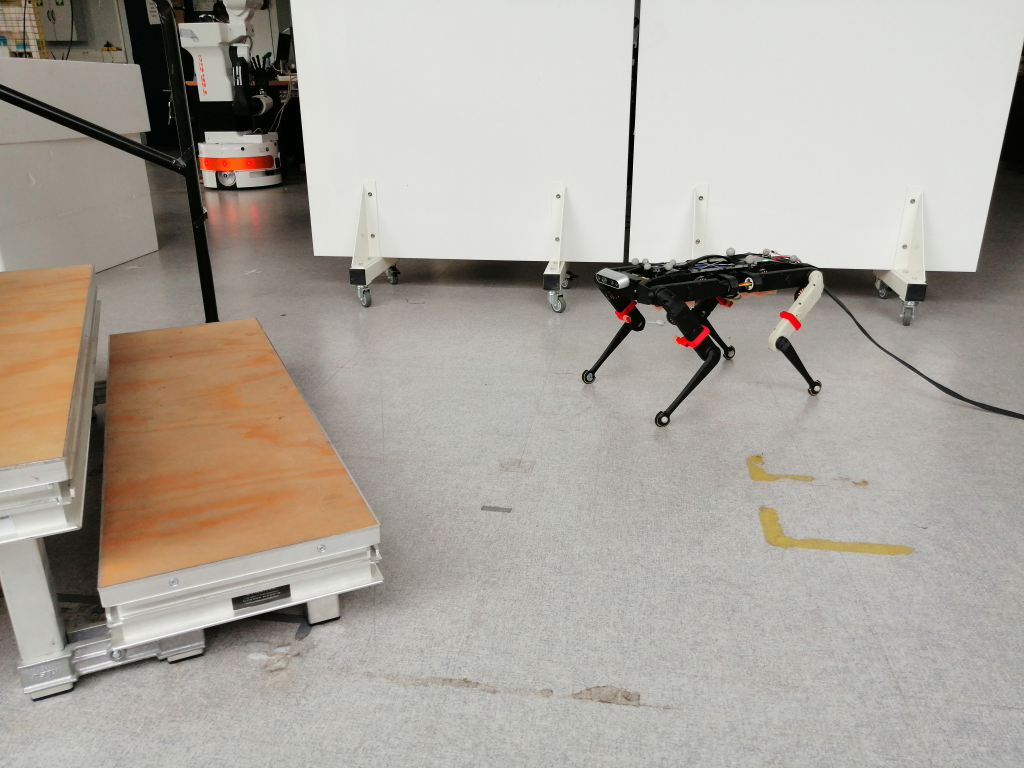
\includegraphics[width=0.80\textwidth]{figures/cosyslam/solo_closer_small.png}
  \caption{Experimental setup: a RealSense D435i is mounted on the Solo robot that localizes itself \wrt stairs. A motion capture system provides ground 
            truth of the robot pose.}
  \label{fig:solo_and_stairs}
\end{figure}

These approaches build metric maps that do not usually leverage the presence of known assets in the scene, although a few examples in the computer vision literature 
exist. In \cite{SalasMoreno2013SLAMSL}, the authors develop one of the first object-level SLAM algorithms from a depth sensor. Using a voting process based on point cloud descriptors, 
a simultaneous recognition and pose estimation of known objects was performed and included as factors in a graph optimization estimator. 
The method benefited from an active search of the objects in the scene, the detection being done in the SLAM loop.
Aside from the robot trajectory and poses of objects, \cite{sucar2020nodeslam} also proposes to optimize the object shapes using a differentiable 
rendering engine. In such approaches, objects need to be detected, classified, and their relative pose \wrt the camera has to be integrated into the estimator. 
On the other end, a work like \cite{pillai2015monocular} uses a semi-dense mono camera SLAM algorithm to produce a scale-ambiguous feature map. 
Then, a descriptor-based multi-view object proposal is performed as a post-processing step. 



% Huge progress to the field of object detection was brought about by the advent of CNN frameworks such as \cite{he2018mask}. As a result, it seems that the domain of 
% object scene reconstruction is now dominated by methods relying only on RGB cameras, for both object detection and pose retrieval. A major example is the framework CosyPose 
% \cite{labbe2020cosypose}. This approach mixes a new state-of-the-art single-view pose estimation algorithm with a multi-view algorithm using RANSAC and Bundle Adjustment. 
% It achieved first in most of the 2020 BOP challenge categories \cite{hodavn2020bop}. This system obtains precision in the order of centimeters on real objects whose 3D 
% model is known. 
% Its performances make it a good candidate as a direct 6D pose sensor to perform the multi-sensor fusion. In the context of legged robots, this is very useful to localize the 
% robot \wrt objects it needs to interact with, such as objects to manipulate or stairs to climb. 
% %However, due to a current lack of generalization capability, the trained models cannot be directly used for objects that are not part of its training.
% While these models are not yet able to be generalized to classes of objects, rapid progress is expected in this direction. Their performances are already very interesting 
% to help with the locomotion in known scenes.

%Another thing that is not handled by CosyPose was the assessment of the uncertainty of measurements from the different objects in the scene, which depends on a variety 
% of parameters such as object occlusion and distance. 
% When considering merging a tracker such as CosyPose with other sensor modalities, an important aspect is to predict covariance representing the level of confidence in 
% the tracker estimate.
% Such data uncertainty awareness has been shown to be crucial to the robustness of SLAM systems involving neural networks subsystems such as \cite{yang2020d3vo}, 
% while \cite{SalasMoreno2013SLAMSL} claimed to compute a covariance matrix approximated as the inverse of the Iterative Closest Point output. The methods targeted for 
% deep learning applications are harder to implement, especially if the goal is to use an off-the-shelf pose estimation neural network, as is the case for this paper. 
% For instance, Bayesian Neural Networks \cite{jospin2020hands} need to be trained explicitly for uncertainty prediction while Monte Carlo (MC) Dropout \cite{gal2016dropout} 
% requires multiple forward passes at run-time.


As described in \secRef{sec:object_pose_est_algos}, deep-learning-based object detection systems have now reached an accuracy that makes them candidates for mobile robotics applications.
Applications range from robot manipulation, like sorting known objects, or localization \wrt known assets. For this last application, however,
the direct output of CosyPose is not sufficient for two reasons. First, many objects have strong symmetries, which makes CosyPose orientation estimation jumps from one to the other
depending on the frames. This output has, therefore, to be filtered using prior knowledge about the world or the robot's movements. Second, the robot needs to keep
a memory of objects it has seen when they go out of its field of view.

We present in this chapter a practical implementation of the proposed MAP formulation fusing inertial measurements and object-level visual features estimated
by CosyPose. The stake is to demonstrate that a centroidal filter is able to merge information typically used for balance control (IMU related)
with features typically needed by a high-level planner, \eg the stair steps locations extracted by the object pose estimator.
Beyond the practical validation for legged robots, this also demonstrates that the single view CosyPose can be extended to a sequential
tracker able to benefit from complementary measurements such as an IMU.

To integrate CosyPose measurements with other sensors, we used the noise model based on empirical data, presented in \secRef{sec:cosypose_covariance}. 
We also detail here the pragmatic implementation of heuristics to circumvent outliers in the network output. 
Experimental validations were conducted with a visual-inertial system, first handheld then mounted on a quadruped robot. Finally, we fine-tuned the pre-trained models 
to perform stairs localization, as explained in \secRef{sec:retraining_with_stairs}. 




\section{Implementation of the Visual Inertial filter}

\subsection{Factor Graph formulation}
This section will be very short so as not to repeat ourselves: the problem has the same structure as the \apriltag-IMU VI system presented in \chpRef{chp:absolute_vi}, 
thus it as the same factor graph \figRef{fig:VI_factor_graph}. The \apriltag\ pose measurement model is replaced by the CosyPose measurement model, presented in \secRef{sec:learning_based_object_pose_est}.


\subsection{Data association and Outlier rejection}
A key part of our SLAM system is the association of landmarks with the rejection of erroneous pose estimates. First of all, each object is associated with a 
label $\alpha$ so that a detection can only match a landmark with the same label. Then, the position of the robot is propagated by integrating the IMU measurements 
with the current biases estimates. Thus, each detected object pose can be transformed in the world frame using the propagated robot state. We check if this pose is 
similar to the one of a landmark with the same label with a threshold on the distance between the poses in $SE(3)$. 
If a detection does not match any landmark then a new landmark is created.

CosyPose can return poses of objects that are not included in the scene because of false detections, of Mask-RCNN, or wrong pose estimations (most often due to object symmetries). 
To handle these outlier detections, each landmark is associated with a score $c$ that corresponds to its repeatability over time: 

\begin{equation}
    c = \frac{n_f}{\Delta t}
\end{equation}

$\Delta t$ is the time since the landmark initialization and $n_f$ is the number of factors associated with it.
The lowest scores are filtered with a threshold determined empirically and the associated landmarks are removed from the map.




\section{Experimental validation}

We have produced datasets in the robotic experimental arena at LAAS-CNRS in Toulouse. This is a 3D environment about $10 m \times 5m$ made of flat floors, 
stairs and beams. The robot environment was augmented with objects of the datasets that were used to train CosyPose. Each dataset is composed of three data sources:

\begin{itemize}
    \item A sequence of RGB images (30 Hz)
    \item A sequence of IMU measurements (200 Hz)
    \item A sequence of motion capture (MoCap) measurements (200 Hz), used as ground truth 
\end{itemize}

We recorded two types of datasets: one for the uncertainty models and one for SLAM experiments. For the uncertainty models, reflective MoCap markers 
were attached to the object to obtain the ground truth of their pose. For the SLAM, only the camera was tracked. We used the monocular RGB camera and the Bosh BMI085 
IMU of an Intel RealSense L515 Camera for handheld trajectories. The Intel RealSense d435i was used with the same modalities 
for the experiments on the quadruped robot Solo \cite{grimminger2020open} as shown in \figRef{fig:solo_and_stairs}. 
The extrinsic calibration between the IMU and the camera was provided by Intel and the delays observed between IMU and Camera measurements were negligible. 
Our datasets are publicly available at \url{https://homepages.laas.fr/mfourmy/icra22_cosyslam}.





\subsection{Object level VI-SLAM}

\begin{figure}[h]
  \centering
  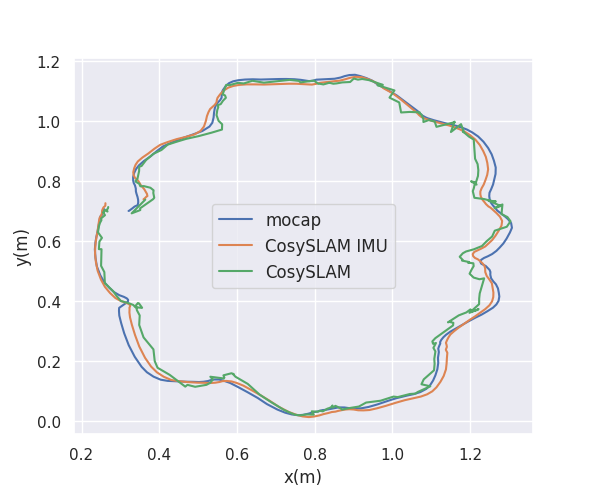
\includegraphics[width=0.9\textwidth]{figures/cosyslam/trajectory_circular.png}
  \caption{Comparison between the MoCap, the output of CosySLAM with visual factors only and the output of CosySLAM with IMU fusion on the circular trajectory.}
  \label{fig:traj_circular}
\end{figure}

In order to validate the performances of the fusion of CosyPose estimates and inertial measurements, we evaluated three scenarios with the camera held by hand and 
T-LESS objects\footnote{T-LESS is one of the datasets for which CosyPose is trained by default and whose object can be bought in the Czech Republic~\cite{hodan17t}. 
It features several small electric devices, whose symmetry at lack of texture make them an interesting benchmark for realistic scenarios.} in the scene. 
The first one is a short and slow trajectory, \ie an ideal scenario. The second one is a slow but long trajectory, to validate the consistency of our system over time. 
The last one is a highly dynamic scenario with a lot of motion that can blur some frames and lose sight of objects for more extended periods. 
Moreover, T-LESS objects being the most difficult objects for pose estimation with CosyPose, they may return many outliers and noisy measurements. 
This is therefore a challenging dataset to test the robustness of our algorithm. \Keyframes\ are selected at 10 Hz, only if objects are detected in the images.

\begin{table}[h]
    \begin{center}
    \caption{Datasets description and results of the hand held videos}
    \label{tab:tless}
    \begin{tabular}{|l|llll|}
        \hline 
        \thead[l]{Scenario}  & \thead[l]{Length(m)} & \thead[l]{Duration(s)} & \thead[l]{MTE¹(cm)} & \thead[l]{STE²(cm)} \\
        \hline 
         V-only - Circular & 3.7 & 23.7 & 3.8 & 1.6\\
        \hline 
         V-only - Short & 2.5 & 12 & 3.8 & 2.4 \\
        \hline 
         V-only - Dynamic & 3.5 & 17.8 & 7.8 & 4.0  \\
        \hline 
         V-IMU - Circular & 3.7 & 23.7 & 1.9 & 0.7\\
        \hline 
         V-IMU - Short & 2.5 & 12 & 1.9 & 0.5 \\
        \hline 
         V-IMU - Dynamic & 3.5 & 17.8 & 1.7 & 1.2  \\
        \hline
    \end{tabular}
    \end{center}
¹ Mean translation error \\
² Standard deviation of translation error
\end{table}

It is interesting to analyze the gains brought by the IMU fusion. The most evident observation is that the output trajectory is smoother, which gives more consistency 
to the result (\figRef{fig:traj_circular}). But we can notice that the mean translation error (MTE) is also reduced (\tabRef{tab:tless}). Indeed, the motion model is more precise thanks 
to IMU data. This makes the outlier rejection more efficient than the visual-only CosySLAM which makes a zero velocity assumption between \keyframes.




\subsection{Localization and Mapping of stairs by Solo}

With our retrained model (\secRef{sec:retraining_with_stairs}) we were able to perform SLAM in our experimental area, without augmenting it with other objects. 
We recorded video sequences including stairs with a camera fixed on a Solo robot (\figRef{fig:map_stairs}). A stair has three discrete symmetries 
that are hard to handle for an object pose estimator and the images provided by Solo were noisy because of the walk. 
These scenarios are challenging for our SLAM system, but it maps successfully the stairs and the error on the position of the base of Solo remains reasonable 
(\tabRef{tab:solo}).

\begin{table}[h]
   \begin{center}
   \caption{Datasets description and results of the videos taken on Solo}
   \label{tab:solo}
    \begin{tabular}{|l|llll|}
        \hline 
        \thead[l]{Scenario}  & \thead[l]{Length(m)} & \thead[l]{Duration(s)} & \thead[l]{MTE(cm)} & \thead[l]{STE(cm)} \\
        \hline 
         V-IMU - Approach & 1.3 & 18.7 & 2.0 & 0.9\\
        \hline 
         V-IMU - Module & 1.3 & 15.5 & 2.4 & 1.5 \\
        \hline
    \end{tabular}
    \end{center}
\end{table}

\begin{figure}[!ht]
  \centering
  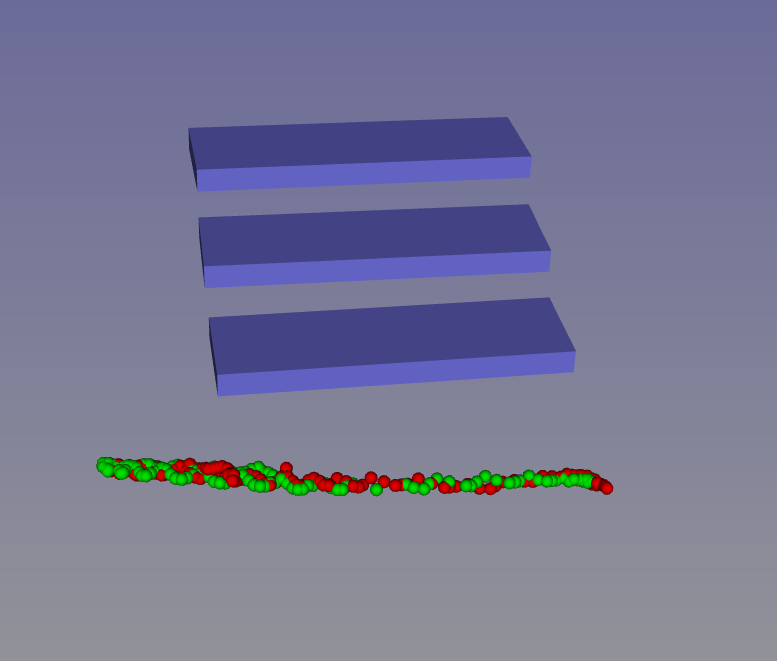
\includegraphics[width=\linewidth]{figures/cosyslam/mapped_stairs.png}
  \caption{This trajectory was recorded on Solo walking along a climbing module made of three stairs using a walking controller \cite{leziart2021implementation}. 
  The green dots represent the trajectory of Solo provided by the MoCap, and the red dots the one produced by our visual-inertial SLAM. 
  The blue rectangles represent the map of the SLAM made of stairs.}
  \label{fig:map_stairs}
\end{figure}




\section{Conclusion}

This chapter presents the first step toward a semantic reconstruction of the robot's environment. We see in this method the potential to provide multi-contact locomotion controllers \cite{carpentier2017multi}
with their needed contact surface reconstructions. By leveraging models of known objects in the scene, one may imagine localizing staircases, their banister, door handles, etc. that
the robot is required to interact with. This work was conducted during the Msc thesis of Cesar Debeunne.

In the case when these object features become sparse, the IMU handles the estimation as a strap-down integration, which is viable for a few seconds. After this delay, extra sources of information are required
to avoid drift in the estimates. One solution would be to increase the robustness of the visual front-end by including residuals using classical 2D salient points features, as visual odometry. In this context,
objects in the scene would be useful both for providing semantic and surface information, as well as providing loop-closures. The covariance model that we developed also requires more development.
In particular, it required important experimental work to build the dataset of CosyPose errors. In particular, needing to collect data for each individual object is very time-consuming. Besides,
the models are likely to overfit the obtained dataset and generalize poorly to datapoints outside of its boundaries.
To improve this, we could work on several aspects. First, the ideal method would be to find a general model, as we did for the AprilTag PnP algorithm (\secRef{sec:apritlag_covariance}), directly computable 
from the CosyPose network. Second, if we show that this is not feasible, we could try to train the covariance model in simulation which provides a vastly superior diversity in situations, though lacking
some of the artifacts of reality. CosyPose itself is only trained in simulation. Thirdly, we could use a Bayesian estimator to fit the uncertainty model, the uncertainty of this model itself in order to 
avoid the particularly bad case of an underestimated covariance. 
%\chapter{Conclusion}

The objective of this thesis was to develop a new class of state estimators for legged robots able to fuse proprioceptive and exteroceptive
sensors. We advocated for the use of tightly-coupled formulations where all measurements and state variables are integrated into a single estimation 
problem. This type of estimator enables a greater accuracy and the estimation of extra parameters by leveraging all sensors correlations.
It also makes use of a sound mathematical formulation to extend generic estimators to more diverse and numerous perception sources, toward whole-body estimation.
The accent was put on the necessary modularity of the formulations to make the mathematical developments extendable to new types of sensors. This 
was achieved through the use of Maximum-A-Posteriori estimation, modeled as Factor Graph optimization. All mathematical formulations used extensively the smooth manifold
and Lie group theories that best represent the geometry of the state variables. We also emphasize the generalizability of the developed measurement models. 

\section{Contributions}

We developed a range of measurement models targeted at sensors present on legged platforms. These measurement models were integrated as factors in 
three factor-graph-based estimators.

We implemented a general factor for camera-based object-level pose estimations based on object pose estimators. 
First, the \apriltag\ library was used 
to \textbf{obtain poses of fiducial markers} used to augment the scene with unique landmarks. We proposed a new analytical model to estimate the covariance of 
these measurements. We discussed the problem of the orientation ambiguity of these markers and proposed a practical method to alleviate this problem.
The anisotropic nature of the pose uncertainty was highlighted in simulated experiments. 
Second, we used \textbf{a deep-learning-based framework to obtain the pose of known objects in the scene}. A covariance model based on empirical data was obtained through
experiments. We showed that we could fine-tune the model to elements of the scene of interest for legged-robots navigation such as stairs.

We then leverage the pre-integration formulation to include high-frequency sensors such as IMU in the factor graph. We propose 
\textbf{a more systematic formulation of this idea, generalizable to other high-rate proprioceptive sensors}. Within this framework, we proposed a new 
IMU pre-integration algorithm \textbf{based on a compact "delta" Lie-group}.
This approach was theoretically compared to the seminal work on IMU pre-integration, based on composite delta Lie groups. 
We then leveraged the generalized pre-integration method to \textbf{extend the pre-integration to force-torque sensors} present at the end-effectors of
legged robots. 
We then proposed a first step toward whole-body estimation, by extending the factor graph approach to also \textbf{estimate centroidal quantities}
(center of mass position and velocity, and angular momentum) by merging centroidal kinematics and force measurements. This makes it possible 
to accurately estimate the centroidal states, despite unavoidable biases in the kinematic model. 


These measurement models were all integrated into the WOLF framework \cite{sola2021wolf} to which we contributed, joining our effort with the IRI team, 
toward an open-source release. WOLF provided the necessary modularity to formulate various estimation problems. 
It then allowed us to implement three different applications of the proposed theory, which we used to experimentally validate our models.

\bigskip

First, we developed \textbf{a visual-inertial SLAM system based on IMU pre-integration and the \apriltag\ pose measurement model}. This estimator was validated through
a series of experiments conducted at LAAS on the \HRP{2} humanoid robot. We showed that the system provided both: localization and mapping with centimetric precision
for the locomotion of the robot on flat terrain and stairs, and a high-rate, smooth estimation of the base velocity. Both were evaluated against a motion capture 
ground truth. 

Second, we proposed \textbf{a tightly-coupled algorithm for simultaneous estimation of the base and centroidal states of the robot}. This estimator combined the pre-integration 
of IMU and force-torque data, centroidal kinematics, and leg odometry. We showed that the estimator enables to estimate the bias on CoM kinematics measurements, which is sometimes ignored
by controllers in first approximation. Experimental validation was conducted on simple trajectories performed on the Solo-12 quadruped robot. 

Third, we implemented \textbf{an object-level visual-inertial SLAM system based on a deep-learning framework for object pose estimation}. This system  used the same 
IMU pre-integration as well as our empirical model of the object pose uncertainty. We showed that the trajectory of the system and objects
in the scene could be recovered and that the IMU contributed to the robustness of the system by alleviating the instability of the pose estimation. We proposed
as a proof of concept to perform visual-inertial SLAM using stairs elements as landmarks, for which we retrained the neural network. This dataset was recorded on the Solo-12 quadruped robot.

Finally, we recorded new datasets on Solo-12 quadruped for following works on the fusion of inertial, kinematics, and vision data. 

\section{Perspectives}
This work laid the foundations of a general factor-graph-based estimation framework for legged robotics. However, a lot of alleys have yet to be explored 
to obtain a usable estimator on any legged platform. Here we present a few of the next projects that we wish to undertake.

\subsection{Short term}
We developed on one hand an object-level visual-inertial system and on the other hand a proprioceptive estimator for the sense of balance. A short-term goal
would be to merge both estimators in one, providing simultaneously a high-rate estimation for control and a non-drifting localization based on SLAM, which should serve also as an input for gait and/or contact planning. 

We began to work in this direction by recording datasets using Solo-12 as an experimental platform. For this experiment, we will concentrate on estimating the 
base state by including inertial, kinematics, and object pose measurements. 

We also plan to integrate the system in a feedback loop with the current controller of Solo-12. For the moment, instabilities in the solver convergence times prevented
us from obtaining a hard-real-time estimate for the proprioceptive estimator, while the \apriltag\ based visual-inertial SLAM system works in real-time. One of the solutions would 
be a hyperparameter search on the numerous options provided by the Ceres solver \cite{ceres-solver}. Another is to search for the most appropriate size of the graph,
that is the frequency of \keyframe\ creation and their number. Marginalization of older states and sparsification procedures should also be investigated.



\subsection{Mid term}

In a second time, we would like to further strengthen the environmental perception of our system. This would be done by developing or integrating a vision system
based on general geometric constraints. Many of the most mature vision-based SLAM systems are based on sparse feature extraction. This will be 
the first venue that we explore. 

Our ideal realization would then be an integrated demo on Solo-12 with an odometry estimator based on kinematics, IMU, and a sparse feature KLT \cite{baker2004lucas} tracking-based 
vision front-end. This system would then easily be extended with either of our object-level SLAM algorithms to provide loop closures and, therefore, a global localization, together
with high bandwidth gravity related state estimation.

The reproducibility of experimental results is a common issue in many scientific fields, which is especially notable in the robotics community. Many benchmarks including 
IMU, vision, and LIDAR sensors are nowadays available \cite{Burri25012016, cortes2018advio, kasper2019benchmark, zhang2021multi}. However, to the best of our knowledge,
very few legged robots datasets are available \cite{fink2020dls, ahmadi2021semi} and none include exteroceptive sensors. The Open Dynamic Robot Initiative \cite{grimminger2020open}, 
through the development of open-hardware robots (such as Solo-12) and open-source low-level controllers aims at making a robotic platform easily accessible to
many institutions. One could imagine that a dataset to benchmark estimation algorithms on such a platform would be useful to the community as a whole. 


\subsection{Longer term}

We will here develop a few ideas and reflections that our work on a general estimator for legged robots inspired.

Following the endeavor to develop an estimator fusing as many sources of information, we could turn our attention to a 
\textit{whole-body} state estimation. As we have seen, the standard proprioception sensor set for legged robots is an IMU attached to the robot base
and encoders at the joints (possibly along with joint torque, motor current, and force sensors at the end effector). This set of sensors
is enough to implement proprioceptive odometry of the base but is quite limited when it comes to perceiving finer information about the state of the robot
and its environment. In particular, the kinesthesis sense of artificial-legged systems is far from the subtleties of their biological counterparts, partly
because of the rigid segment assumptions. One solution is to augment the robot with other sensors measuring these flexibilities. Recent solutions have demonstrated
the applicability of such methods by placing IMUs in each segment of an exoskeleton. One might also imagine adding strain gauges to measure directly 
the segments' deflections. 

The sense of touch is for the moment also underrepresented in legged robotics. Some teams propose to add
artificial skins that are implemented as strain cells sheets, which provides a higher density haptic feedback than strain-gauges. 
These systems in particular demonstrated a great potential for human-robot interactions. 
A higher-quality sense a touch may also provide richer information about the nature of the contacts between the robot and its environment, be it for locomotion
(slip detection, terrain nature, etc.), or for manipulation (object surface analysis, 3D object position estimation). 

On the other end of the spectrum, one could imagine methods targeted toward robots with limited sets of sensors that
an observability study based on our formulation would help to optimize. For instance, Solo-12 is too small to be 
equipped with high-fidelity, multiple-axis strain gauges such as those found on humanoid robots. Such a robot may be equipped with cheap
one-dimensional strain-gauges, which would require new measurement model formulations, with application in centroidal estimation.

With a limited set of sensors, the choice of their nature and placement on the robotic platform is crucial, which is limited by the nature of its initial design. 
On the control side, the concept of co-design is gaining traction. The goal is
to optimize the design of a robot to certain criteria, such as energy efficiency or dynamic capabilities, exploring the design space guided by 
the simulated control of the platform. A dual concept could be applied to optimize the design of the platform to maximize the efficiency of estimation algorithms.

Our visual-inertial SLAM work based on CosyPose object position is a first step in deriving semantic information from the environment. On this line of research, we may imagine
including more general information about the scene objects by leveraging latent space representations of these deep-learning algorithms. This might enable us to deal with the problem
caused by the symmetries of these objects more properly. Work is also currently conducted on the side of the CosyPose team to better generalize the pose estimation to objects on which the 
model has not been trained. More broadly, the dialog between trained models and optimal estimation has a lot of potentials, both in robotics
and computer vision communities. On one hand, learned factors could be trained with the end goal of improving the result of the estimation algorithm. On the other end,
injecting priors based on physical models of the world, such as the dynamics of legged systems, can be used to improve the results of vision-based algorithms
for dynamic scenes and human pose reconstruction.

% In the context of legged robot locomotion, we showed that systems such as CosyPose were useful to aid the navigation of legged robots with 

Finally, the notion of state feedback may be rethought entirely. Model-based controllers rely on a limited set of physically grounded states to compute the robot control inputs. 
However, some recent learning-based systems do not require this kind of information, relying instead on latent space representations of the robot state learned
in simulation. Some of these algorithms abstract the concepts of robot and environment as a single latent state vector resulting from a tight coupling of raw proprioceptive and exteroceptive
measurements. While demonstrating impressive results in practice, those representations might have the downside of not being interpretable by a human operator and other systems, 
making the communication and fault detection harder to manage.  



% \appendix




\chapter{Covariance of the estimate}
\label{chp:MAP_covariance}
An important question to ask is how confident are we in our MAP estimate.
This can inform us on the quality of the performed estimation. In particular, in the case of parameter identification, a certain degree of excitation,
namely variability in the data, is necessary to obtain reliable values. Unfortunately, as we will see, the computation of the covariance on the posterior
is a costly process that is, therefore, rarely used in online estimation.

First we will review the process to obtain the posterior's covariance, known as the Laplacian approximation. Then we will give a simple example to
illustrate the nature of the approximation and compare it to an exact inference of the posterior distribution.

\section{Laplace approximation}
\label{sec:map_covariance}
Even if our priors and measurements models are Gaussian distributions, the posterior distribution
is in general non-Gaussian (unless all measurements models are linear). The region near the peak of the posterior is, however, often nearly Gaussian in shape.
The curvature around the mode is described by the Hessian of the posterior negative log-likelihood at the MAP estimated state. 
It can be shown that he Hessian is the \textit{information matrix} of the problem\footnote{The proof of this statement is out of the scope of this document and can be found in Section 5.1 of
\cite{peng2018advanced}}. Thus, finding the covariance of the MAP estimate resolves to inverting a 
sparse positive definite matrix.

\begin{equation}
    p(\cX | \cZ) \approx \Gaussian{\cX^{MAP}}{\bfH^{-1}}
    \label{eq:map_laplace}
\end{equation}

This is referred to as the quadratic or Laplace approximation (\cite{mcelreath2018statistical}, section 2.4.2). Obtaining an approximation of the full posterior is then a two-step process: 
first, find the mode of the posterior (the MAP), then "fit a Gaussian" on this mode. 

The full covariance is however rarely computed for a few reasons. First, few algorithms rely on this information (a notable exception being active feature matching \cite{davison2007monoslam}, which is not longer used in state of the art vision systems). Second, computing the Hessian's inverse is too costly to be realized "in the loop". Sometimes, only parts of the covariance are computed using the Schur-complement method \cite{konolige2005slam}, which is costly but much less than the full inverse.
The covariance computation is then often left for offline evaluations of the estimation.

To contrast this approach with the aforementioned approximations, variational inference as applied in Barfoot et al. 
\cite{barfoot2020exactly} for instance fit both the mean and the information matrix of a Gaussian model as a result of a single optimization problem.



\section{Example: stereoscopic depth estimation}

We can illustrate the Laplace approximation with a one-dimensional toy problem (borrowed from Barfoot \cite{barfoot2017state}, section 4.1.1).
The problem is stated as estimating the depth $x \in \Reals$ of a landmark in the scene with a nonlinear camera model (see \figRef{fig:barfoot_stereo})
%
\begin{equation}
    y = \frac{fb}{x} + n_y
\end{equation}
%
%
\begin{figure}[h]
    \centering
    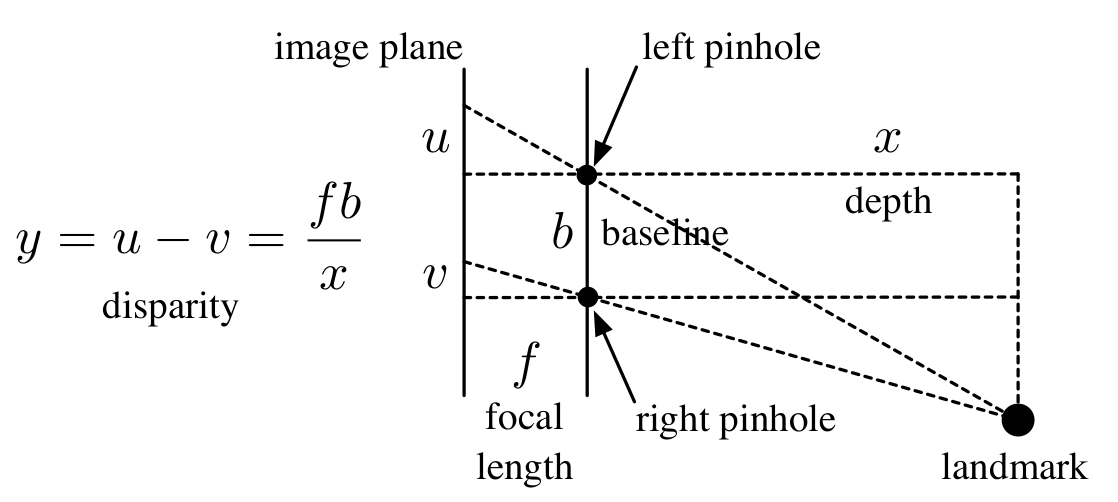
\includegraphics[width=0.6\textwidth]{figures/barfoot_stereo.png}
    \caption{Stereo depth estimation toy model \cite{barfoot2017state}}
    \label{fig:barfoot_stereo}
 \end{figure}
%
where $y=u - v$ is a disparity measurement ($u$ and $v$ are pixels corresponding to the projection of the landmark in each camera), $f$ is the focal
length of the cameras (in pixels), $b$ is the horizontal distance between cameras (the baseline, in meters), and $n_y \approx \Gaussian{0}{\sigma_y^2}$ 
is the measurements noise (in pixels), assumed to be Gaussian. We also assume that we have prior knowledge about the 
estimated value $x_p$, with a standard deviation of $\sigma_p$.

To ground the problem, we will assign sensible values to the problem (same as \cite{barfoot2017state}):
%
\begin{gather*}
    x_{true} = 22~m, \quad x_p = 20~m, \quad \sigma_p = 3~m \\
    f = 400~pixels, \quad b = 0.1~m, \quad \sigma_y = 0.3~pixels   
\end{gather*}
%
where $x_{true}$ is the true depth that we seek to estimate.

Notice that the prior standard deviation is quite big, assuming a great uncertainty about the prior value. We simulate noisy measurements by drawing samples 
$\{y_{i \in [1..m]}\}$ of the measurement model using $x_{true}$ (we drew $m=10$ measurements). For a low dimensional problem such as this one, 
it is possible to compute the full posterior distribution $p(x|\bfy)$ by numerical integration, which is referred to as the "grid approximation" by 
\cite{mcelreath2018statistical}. We can make this computation almost arbitrarily precise since the computations are quite cheap. The prior and density distribution are represented in \figRef{fig:MAP_stereo1D}. Applying the Laplacian approximation to
compute a posterior approximation involves minimizing the negative log-likelihood:

\begin{equation}
    \frac{1}{2 \sigma_p^2}(x - x_p)^2 + \frac{1}{2\sigma_y^2} \sum_{i=1}^m (\frac{fb}{x} - y_i)
\end{equation}

Finding the MAP and approximating the covariance deviation of $x$, we can plot the MAP posterior along with its numerical computation in \figRef{fig:MAP_stereo1D}. 
Both computations result in largely overlapping functions: the main mass of the real posterior density function is captured by the Laplacian approximation.
However, notice that the real posterior distribution is not symmetrical contrary to the prior it derives from. This means that, contrary to its Gaussian approximation, the mean of the
of the real posterior is not equal to its mode. 

\begin{figure}[h]
    \centering
    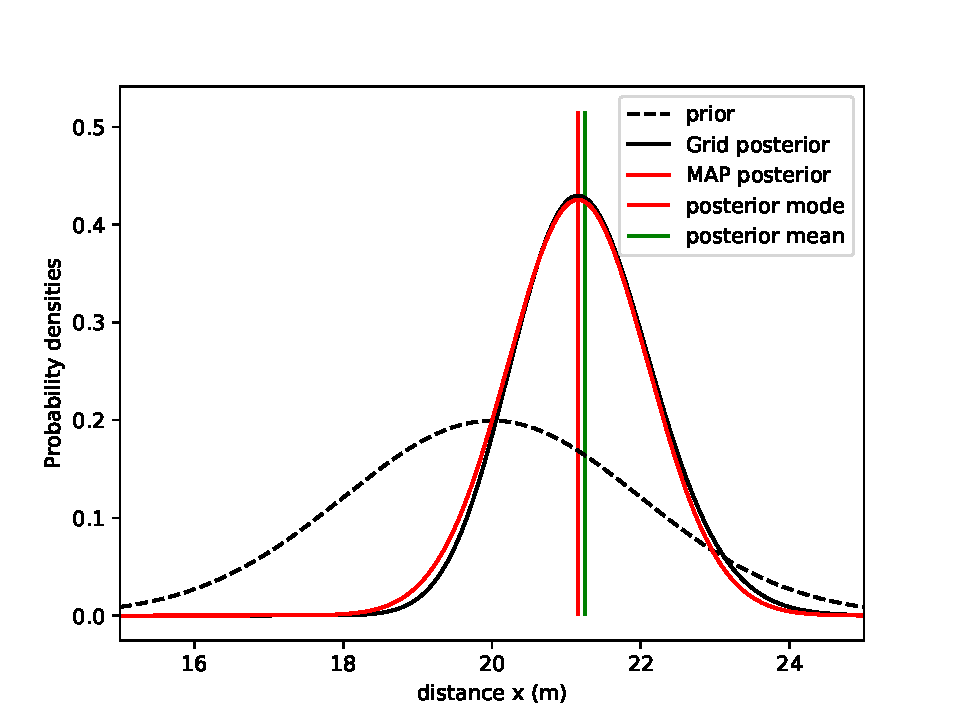
\includegraphics[width=0.8\textwidth]{figures/MAP_stereo1D.pdf}
    \caption{Representation of the posterior distribution inference for the 1D depth estimation problem. Dotted black: prior on $x$, 
    continuous black: numerical "grid" integration of the posterior, continuous red: Laplacian approximation of the posterior. 
    Vertical lines: red=MAP, green=mean of the posterior. The true value (22 m) is reasonably close to the MAP given the variance 
    of the posterior distribution.
    }
    \label{fig:MAP_stereo1D}
 \end{figure}







\chapter{Pre-integration details}
\section{Justification of \cite{forster2017-TRO} delta formulas}
\label{sec:forster_proof}
We detail here how the delta formulas of equation \eqRef{eq:IMUPreintij} can be derived from \eqRef{eq:IMUIntim}.

The rotation one is easy to get, multiplying by $\Rot{}{}^{i,T}$:
\begin{equation}
    \DR_{im} \triangleq \Rot{}{}^{i,T} \Rot{}{}^{m} = \prod_{k=i}^{m} \Exp((\angvelm{}{}^k - \bias_{\angvel{}{}}^k - \noise_{\angvel{}{}}^k)\dt)
    \label{eq:IMUDeltaR}
\end{equation}

The velocity is as well quite easy, by defining $\Dt_{im} \triangleq \sum_{k=i}^{m} \dt = (m-i)\dt$:
\begin{equation}
    \Dv_{im} \triangleq \Rot{}{}^{i,T} (\vel{}{m} - \vel{}{i} - g \Dt_{im}) 
    = \prod_{k=i}^{m} \DR_{ik} \Exp((\accm{}{}^k - \bias_{\acc{}{}}^k - \noise_{\acc{}{}}^k)\dt)
    \label{eq:IMUDeltav}
\end{equation}

The position delta requires more calculations. First, inject equation \eqRef{eq:IMUDeltav} in the position equation of \eqRef{eq:IMUIntim} then rearrange and reorder the terms.

\begin{equation}
\begin{split}
\posi{}{}^{m} - \posi{}{}^{i} &= \sum_{k=i}^{m} \Big[
(\vel{}{}^i + \grav \Dt_{ik} + \Rot{}{}^i \Dv_{ik})\dt 
+ \frac{1}{2}\grav \dt^2 + \frac{1}{2}\Rot{}{}^{k}(\accm{}{}^k - \bias_{\acc{}{}}^k - \noise_{\acc{}{}}^k)\dt^2 \Big]
\\
&= \vel{}{}^i \Dt_{im} + 
\grav\sum_{k=i}^{m} \Dt_{ik} \dt + \frac{1}{2}\grav \sum_{k=i}^{m} \dt^2 +
\Rot{}{}^i\sum_{k=i}^{m} \Big[\Dv_{ik}\dt +  \frac{1}{2} \DR_{ik} (\accm{}{}^k - \bias_{\acc{}{}}^k - \noise_{\acc{}{}}^k)\dt^2 \Big]
\\
&= \vel{}{}^i \Dt_{im} + 
\grav \sum_{k=i}^{m} (\Dt_{ik} \dt + \frac{1}{2}\dt^2) +
\Rot{}{}^i\sum_{k=i}^{m} \Big[\Dv_{ik}\dt +  \frac{1}{2} \DR_{ik} (\accm{}{}^k - \bias_{\acc{}{}}^k - \noise_{\acc{}{}}^k)\dt^2 \Big]
\end{split}
\end{equation}

We will simplify the gravity term that we will call $\cG t_{im}$. Noting that:

\begin{equation*}
    \sum_{k=i}^{m}k = \sum_{k=1}^{m}k - \sum_{k=1}^{i-1}k = \frac{m(m-1)}{2} - \frac{i(i-1)}{2} 
\end{equation*}

we can deduce that:

\begin{equation*}
\begin{split}
\cG t_{im} 
&= \dt \sum_{k=i}^{m}(\Dt_{ik} + \frac{1}{2}\dt) = \dt \sum_{k=i}^{m}((k -i)\dt + \frac{1}{2}\dt)
\\
&= \dt \Big[ \sum_{k=i}^{m} [ k \dt - i(m-i)\dt ] + \frac{1}{2}\Dt_{im}  \Big] 
\\
&= \dt \Big[ \frac{\dt}{2} (m(m-1) - i(i-1) - 2i(m-1)) + \frac{1}{2}\Dt_{im} \Big] 
\\
&= \dt \Big[ \frac{\dt}{2} (i^2 - 2im + m^2 + i - m) + \frac{1}{2}\Dt_{im} \Big] 
\\
&= \dt \Big[ \frac{1}{2} (m-i)^2dt - \frac{1}{2}(m - i)\dt + \frac{1}{2}\Dt_{im} \Big]
\\
&= \frac{1}{2} (m-i)^2dt^2 = \frac{1}{2} \Dt_{im}^2
\end{split}
\end{equation*}
Multiplying by $\Rot{}{}^{i,T}$ and reordering the terms, we can finally define a position delta quantity:

\begin{equation}
    \Dp_{im} \triangleq \Rot{}{}^{i,T}(\posi{}{}^m - \posi{}{}^i - \vel{}{}^i \Dt_{im} - \frac{1}{2} \grav \Dt_{im}^2) = 
    \sum_{k=i}^{m} \Big[\Dv_{ik}\dt +  \frac{1}{2} \DR_{ik} (\accm{}{}^k - \bias_{\acc{}{}}^k - \noise_{\acc{}{}}^k)\dt^2 \Big]
\end{equation}


\section{Elements of the IMU delta matrix Lie group}
\label{sec:IMULieGroup}

\subsection{Tangent space and Lie algebra \texorpdfstring{$\mathfrak{d}$}{d}}
\cite{sola2018micro}
Following \cite{sola2018micro}, the tangent space of $\cD$ at the point $\D$ is found by taking the time derivative of the group constraint, $\D\inv\D = \bfI$.
Noting $\dot{\bullet} \te \dpar{\bullet}{t}$, this yields 
% the tangent space constraint, $\D\inv\dot\D+\dot{(\D\inv)}\D=0$.
% This gives 
after a few manipulations
%
\begin{align}\label{equ:constr}
\D\inv\dot\D 
&=
\begin{bsmallmatrix}
\hatx{\bw} & ~~\DR\tr\bfa~~ & \DR\tr(\bfv-\Dv) \\
\bf0 & 0 & 1 \\
\bf0 & 0 & 0 
\end{bsmallmatrix}
~,
\end{align}
%
with $\bfv \te \dot\Dp$, $\bfa \te \dot\Dv$ and $\hatx{\bw} \te \DR\tr\dot\DR$.
% The equation above defines the tangent space at the point $\D$. 
The Lie algebra $\mathfrak{d}$ is the tangent space at the identity $\D=\bfI$.
Its elements $\bm\nu\hhat 
\te \dot\D |_{\D=\bfI}$ and their isomorphics $\bm\nu$ in Cartesian space are given by, % $\D=\bfI$, so
%
\begin{align}
\bm\nu\hhat 
% \te \dot\D |_{\D=\bfI}
&=
\begin{bsmallmatrix}
\hatx{\bw} & \bfa & \bfv \\
\bf0 & 0 & 1 \\
\bf0 & 0 & 0 
\end{bsmallmatrix} \in \mathfrak{d}
~~~\xrightleftharpoons[\wedge]{~\vee~}~~~ 
\bm\nu=\begin{bsmallmatrix}
\bfv \\ \bfa \\ \bw \\ 1
\end{bsmallmatrix} \in\bbR^{10}
~.
\end{align}
%
This tangent $\bm\nu\hhat$ corresponds to the `velocity' of the group element. 
Any point in the Lie algebra can be obtained after moving at constant velocity during a period $\Dt$, that is, $\bftau\hhat=\bm\nu\hhat\Dt\in\mathfrak{d}$ ---see \eqRef{equ:lie_algebra}.
%
\subsection{The exponential map}
\subsubsection{The general case}
Eq.~\eqRef{equ:constr} can be written as $\dot\D=\D\cdot\bm\nu\hhat$.
This is an ordinary differential equation whose  integral for constant $\bm\nu$ yields the exponential map \cite{sola2018micro}, $ \D(t) = \exp\left(\bm\nu\hhat t\right)$.
This gives a direct expression of the integral of information of the type $(\bfv,\bfa,\bw)$ onto the deltas manifold. See below for the $(\bfa,\bw)$ case.
The closed form of the exponential map is obtained through Taylor expansion (see \eg\ \cite{sola2018micro}\ for examples). 
At $t=\Dt$ we have,
%
\begin{align}
\D(\Dt) 
&= \exp(\bm\nu\hhat\Dt) \te \sum_n \frac1{n!}(\bm\nu\hhat\Dt)^n
~.
\end{align}
%
% with $\bfA=\bftau\hhat\Dt$.
%
Exploiting the cyclic pattern of the powers of $\hatx{\bw}$, this results in
%
\begin{align}
\exp\left(\begin{bsmallmatrix}
\hatx{\bw} & \bfa & \bfv \\
\bf0 & 0 & 1 \\
\bf0 & 0 & 0 
\end{bsmallmatrix}\Dt\right) 
\!=\! \begin{bsmallmatrix}
\exp(\hatx{\bw}\Dt) & \bfQ\bfa\Dt\, & \bfQ\bfv\Dt+\bfP\bfa\Dt^2 \\
\bf0 & 1 & \Dt \\
\bf0 & 0 & 1
\end{bsmallmatrix}
\end{align}
%
with (we skip proofs for space reasons)
%
\begin{align} \label{equ:RQP}
% \bfR (\bth)
%  &= \exp(\hatx{\bth})
%   = \bfI + \sin\theta\hatx{\bfu} + (1-\cos\theta)\hatx{\bfu}^2\\
\bfQ (\bth)
 &= 
  \bfI + \frac{1-\cos\theta}{\theta}\hatx{\bfu} + \frac{\theta-\sin\theta}{\theta}\hatx{\bfu}^2\\
\bfP (\bth)
 &= 
  \frac12\bfI 
   + \frac{\theta-\sin\theta}{\theta^2}\hatx{\bfu} 
   + \frac{\cos\theta + \frac12\theta^2 - 1}{\theta^2}\hatx{\bfu}^2
~,
\end{align}
%
where  $\bth=\bw\Dt$, $\theta=\norm{\bth}$ and $\bfu=\bth/\theta$ form the angle-axis representation of the rotation step $\bw\Dt$. 


\subsubsection{The IMU case of \texorpdfstring{$\bfv=0$}{bfv=0}}
\label{sec:IMU_case}

We defined the IMU deltas as the motion relative to the free-falling frame, which has initial velocity $\bfv_i$. 
Thus the tangent velocity $\bfv=\dot\Dp$  is zero at the start of the integration step. 
%
Since the exponential $\Exp(\bm\nu\Dt)$ assumes a constant tangent vector $\bm\nu=(\bfv,\bfa,\bw,1)$ during the interval $\Dt$, we have that $\bfv=0$ during the full step. 
%
This gives immediately
%
\begin{align}
% \D &= 
\exp\left(\begin{bsmallmatrix}
\hatx{\bw} & \bfa & \bf0 \\
\bf0 & 0 & 1 \\
\bf0 & 0 & 0 
\end{bsmallmatrix}\Dt\right) 
= \begin{bsmallmatrix}
\exp(\hatx{\bw}\Dt) & ~\bfQ\bfa\Dt~ & \bfP\bfa\Dt^2 \\
\bf0 & 1 & \Dt \\
\bf0 & 0 & 1
\end{bsmallmatrix}
~.
\end{align}




\subsection{The adjoint and small adjoint matrices}

%
Following the general methodology explained in \cite{sola2018micro}, the adjoint matrix is obtained by identifying the linear terms in $\Ad{\D}\bftau=(\D\bftau\hhat\D\inv)\vvee$. We get after long but relatively easy calculations,
%
\begin{align}\label{equ:Ad}
\Ad{\D} &=
\begin{bsmallmatrix}
\DR & -\DR\Dt & \hatx{\Dp-\Dv\Dt}\DR & \Dv \\
\bf0 & \DR & \hatx{\Dv}\DR & \bf0 \\
\bf0 & \bf0 & \DR & \bf0 \\
\bf0 & \bf0 & \bf0 & 1
\end{bsmallmatrix} 
\quad
\in\bbR^{10\times10}~.
\end{align}



Similarly, from \cite{EADE-18-DERIVATIVE} the small adjoint matrix can be computed by identifying the linear terms in $
\ad{\bftau}\bfsigma = 
(\bftau\hhat\bfsigma\hhat-\bfsigma\hhat\bftau\hhat)^\vee
$
%
which  for $\bftau=(\bfrho,\bfupsilon,\bth,\Dt)\in\mathfrak{d}$ yields,
%
\begin{align}\label{equ:ad}
\mathrm{\bf ad}_\bftau = \begin{bsmallmatrix}
\hatx{\bth} & -\bfI\Dt & \hatx{\bfrho} & \bfupsilon \\
\bf0 & \hatx{\bth} & \hatx{\bfupsilon} & \bf0 \\
\bf0 & \bf0 & \hatx{\bth} & \bf0 \\
\bf0 & \bf0 & \bf0 & 0 
\end{bsmallmatrix}
\quad
\in\bbR^{10\times10}~.
\end{align}




\subsection{The right Jacobian}

The right Jacobian $\mjac{}{r}$ is the Jacobian of $\Exp()$ as described in \cite{sola2018micro}.
Lacking at the moment a closed form for it, we take the general methodology for the left Jacobian described in \cite{EADE-18-DERIVATIVE}, and transform it to the right using $\mjac{}{r}(\bftau)=\mjac{}{l}(-\bftau)$ \cite{sola2018micro},
%
\begin{align}\label{equ:Jr}
\mjac{}{r}(\bftau) 
= \mjac{}{l}(-\bftau) 
= \sum_i \frac{\ad{-\bftau}^i}{(i+1)!}
= \sum_i \frac{(-\ad{\bftau})^i}{(i+1)!}
% ~
% \in\bbR^{10\times10}
~.
\end{align}
%
This sum can be truncated at the desired degree of accuracy.






\section{Jacobians of force/torque pre-integration}

TODO



% \listoffigures
% \listoftables

% \newpage

\noindent\makebox[\linewidth]{\rule{0.6\textwidth}{2pt}}

\small

\paragraph{Abstract}~

Legged robots are complex mechanisms whose stable behavior depends on the proper estimation of several different quantities that must be observed at 
high speed and accuracy. While the robot state can mostly not be observed directly by any existing sensors, it is typically reconstructed by fusing very 
diverse sensor modalities.
These sources of information differ significantly on their acquisition frequencies, the nature of the data, and the computational processing cost. 
While state estimation by sensor fusion is a common topic to most robotic platforms, it offers a particular challenge in legged robotics by their peculiar dynamics.
For legged robots, on the one hand, the robot state is needed to maintain its sense of balance and locomote safely, and, on the other hand, a precise representation 
of the environment is required for navigation and interaction. 

The current approach for many legged systems, in the literature, solve
these problems independently, using cascades of estimators that may neglect some of the correlation present in the data.
This artificial decoupling acts as strong priors that enable simple estimators to handle the estimation of each part of the cascade and stabilize 
the behavior of the overall estimation scheme. On the other hand, designing a cascade involves a lot of specialized work that hardly generalizes to new 
scenarios or new sensor modalities.
In this thesis, we rather defend the idea of building a single tightly-coupled estimator capable of estimating all quantities needed by the robot. 
For this goal, the framework of a-posteriori estimation, formalized as a factor graph, is very suitable. This assertion does not come as a surprise, 
as factor graphs are nowadays highly popular in the SLAM literature, yet they are still under-represented in legged robots systems.

In this thesis, we investigate a few avenues that we believe are crucial to achieving these goals. First, we develop tailored sensor measurement models 
with attention to the correct mathematical formulation involving Lie theory.
Second, we propose visual-inertial systems based on object-level detection that provide relative transformation between the camera and the objects.
We provide covariance models for two kinds of objects: the first one is an analytical model for fiducial markers~; the second
is an empirical model for deep-learning-based object pose estimation.
Third, we handle high-rate sensors by developing a generalization of the IMU pre-integration theory. We propose a new formulation of the IMU
pre-integration based on compact Lie groups. 
Fourth, we show that pre-integration can also be applied to use force-torque sensors found on legged robots. 
By fusing it with a leg-kinematics based odometry and IMU, we show that this new formulation makes possible the tightly-coupled estimation
of centroidal quantities within the context of Factor Graph estimation.

The proposed theoretical ideas are implemented in a coherent estimation framework, extending the factor-graph software Wolf. Each new modality is 
validated in a dedicated experimental setup that allowed us to quantify its interest and relevance for legged robotics.



\paragraph{Keywords}~

Factor Graph, estimation, legged robots, SLAM, pre-integration, IMU, force sensor, vision 

\noindent\makebox[\linewidth]{\rule{0.6\textwidth}{2pt}}



\newpage


\noindent\makebox[\linewidth]{\rule{0.6\textwidth}{2pt}}


\paragraph{Résumé}~

Les robots à pattes sont des mécanismes complexes dont la stabilité dépend de la bonne estimation de plusieurs quantités 
qui doivent être observées à grande vitesse et avec précision. Bien que l'état du robot ne puisse généralement pas être observé directement par 
des capteurs, il est généralement possible de le reconstruire en fusionnant plusieurs capteurs à condition d'être capable de
bénéficier des modalités très diverses qu'ils offrent.
C'est bien sur un sujet commun à la plupart des plateformes robotiques, mais le défi posé par l'estimation d'état par fusion de capteurs
se renouvelle dans le cadre de la robotique à patte à cause de la dynamique particulière de ces systèmes. D'une part, leur équilibre
dépend intimement de l'estimation correcte de leur état~; d'autre part, ils ont besoin d'une représentation fine de leur environnement
pour y naviguer et y interagir.

A ce jour, l'approche actuelle dominante les robots à pattes est de résoudre
indépendamment plusieurs problèmes d'estimation, en utilisant des cascades d'estimateurs qui peuvent négliger une partie des corrélations présente dans les données.
Ce découplage artificiel agit comme des \textit{a priori} forts qui permettent à des estimateurs simples de gérer chaque partie de la cascade et de stabiliser 
le comportement du schéma d'estimation global. Ce pragmatisme implique néanmoins beaucoup de travail spécialisé qui ne se généralise guère à de 
nouveaux scénarios ou à de nouvelles modalités de capteurs.
Dans cette thèse, nous défendons l'idée de construire un unique estimateur capable d'estimer toutes les quantités nécessaires au robot de manière étroitement couplée.
Le cadre de l'estimation a-postériori, formalisé sous la forme d'un graphe de facteurs, est alors très approprié pour formaliser l'approche. Cette affirmation n'est pas une surprise, 
car les graphes de facteurs sont aujourd'hui très populaires dans la littérature SLAM. Ils sont cependant encore sous-représentés pour les robots à pattes.

Dans cette thèse, nous étudions quelques pistes qui nous semblent cruciales pour atteindre cet objectif. Tout d'abord, nous développons des modèles de mesure de 
capteurs en prêtant attention à la formulation mathématique correcte fondée sur la théorie des groupes de Lie.
Deuxièmement, nous proposons des systèmes visuels inertiels basés sur des algorithmes de détection d'objets, qui fournissent une transformation relative entre la caméra 
et les objets.
Nous fournissons des modèles de covariance pour deux types d'objets~: le premier est un modèle analytique pour les marqueurs fiduciaires~; la deuxième
est un modèle empirique pour l'estimation de pose d'objet basée sur l'apprentissage en profondeur.
Troisièmement, nous traitons les capteurs à haute fréquence en développant une généralisation de la théorie de pré-intégration IMU. Nous proposons une nouvelle 
formulation de la pré-intégration IMU basée sur des groupes de Lie compacts.
Quatrièmement, nous montrons que la pré-intégration peut également être appliquée pour utiliser les capteurs de forces trouvés sur les robots à pattes.
En la fusionnant avec une odométrie basée sur la cinématique des jambes et une IMU, nous montrons que cette nouvelle formulation rend possible l'estimation 
étroitement couplée des quantités centroïdale dans le contexte de l'estimation des graphes de facteurs.

Les idées théoriques proposées sont mises en œuvre dans un cadre d'estimation cohérent, étendant le logiciel de graphe de facteurs Wolf. 
Chaque nouvelle modalité est validée dans un montage expérimental dédié qui nous a permis de quantifier son intérêt et sa pertinence pour la robotique à pattes.


\paragraph{Mots clefs} ~

Estimation, graphes de facteurs, robots à pattes, SLAM, pre-integration, IMU, capteur de force, vision 


\noindent\makebox[\linewidth]{\rule{0.6\textwidth}{2pt}}

\normalsize

\printbibliography
\end{document}
